% !TEX program = LuaLaTeX
%\errorcontextlines 10000
\DocumentMetadata{testphase={latest,math,table},lang=en}
\providecommand{\tagpdfsetup}[1]{}
\tagpdfsetup{math/alt/use = true}
\nonstopmode
%\RequirePackage[l2tabu, orthodox]{nag}
%\documentclass{article}
\documentclass[10pt]{book}

\usepackage[aux]{rerunfilecheck}

\usepackage{etoolbox}

\PassOptionsToPackage{HTML}{xcolor}
%\usepackage[HTML]{xcolor} % must occur before qrcode in apex_style
\usepackage{tikz}
\usetikzlibrary{calc}

% with 10pt font, 1em ~ 10pt ; 1ex ~ 4.3pt

%%Page Size stuff

\usepackage[paperheight=11in,paperwidth=8.5in,%
	inner=1in,textheight=7in,textwidth=320pt,marginparwidth=150pt,%
	marginparsep=32pt,bottom=3in,footskip=1.5in]{geometry}

\newcommand{\exercisegeometry}{%
%	\batchmode%
	\newgeometry{inner=72pt,outer=72pt,textheight=9.25in,tmargin=.75in,
		marginparwidth=150pt,marginparsep=32pt,footskip=29pt}%
%	\errorstopmode%
}
\newcommand{\eendgeometry}{%
%	\batchmode%
	\newgeometry{inner=72pt,outer=36pt,textheight=10in,
		marginparwidth=150pt,marginparsep=32pt}%
%	\errorstopmode%
}
\newcommand{\prefacegeometry}{%
%	\batchmode%
	\newgeometry{inner=1in,textheight=9in,textwidth=320pt,marginparwidth=150pt,%
		marginparsep=32pt,bottom=1in,footskip=1.5in}%
%	\errorstopmode%
}

\newlength{\widest}

%%% This was originally a style with \usepackage, but inputing is generally
%%% equivalent.  The only real difference is how latexml handles style files.
%%% So we'll input this document as a header instead,
%%% and save \usepackage{customstyle}
%%% for things latexml is having trouble with.
%%% This does mean that the distinction between APEX_format and Header_Calculus
%%% is no longer important, and mostly historical.

% do we want to print the keys for the labels? if so, uncomment
%\usepackage[notref,notcite]{showkeys}

\usepackage{amsthm}
\usepackage{amsmath}
%\usepackage{amssymb} % todo ? https://tex.stackexchange.com/a/3000/107497 recommends dropping amssymb in favor of unicode-math
% but then the font loading gets messed up with mathspec
% see also https://tex.stackexchange.com/q/218112/107497 that if the font doesn't have math, then it's a losing battle
%\RequirePackage{unicode-math}

\usepackage{graphicx}
\usepackage{multicol}
\usepackage{makeidx}

\usepackage[normalem]{ulem}

\usepackage{calc}
\usepackage{ragged2e}

%\usepackage[inline]{enumitem}
\usepackage{enumext}

\usepackage[nocomments]{latexml}
\lxDocumentID{apex}

\numberwithin{figure}{section}
\numberwithin{equation}{section}

%%%%%%%%%%%%%%%%%%%%%

\makeindex

\newcommand{\apex}{\texorpdfstring{A\kern -.1em \lower -.5ex\hbox{P}\kern -.25em\lower .5ex\hbox{E}\kern -.1em X}{APEX}}


% Create boolean for whether or not to print 3D graphics. 
% Also creates command to switch back and forth; "looks better."
\newtoggle{in_threeD}
\newcommand{\usethreeDgraphics}{\toggletrue{in_threeD}}
\newcommand{\usetwoDgraphics}{\togglefalse{in_threeD}}
\usethreeDgraphics


\usepackage{pgfplots}
\pgfplotsset{compat=1.8}

\newtoggle{inColor}
\toggletrue{inColor}

\pgfplotsset{colormap={coloronemap}{rgb=(.4,.4,1); rgb=(.8,.8,1)}}
\pgfplotsset{colormap={colortwomap}{rgb=(1,.4,.4); rgb=(1,.8,.8)}}
%\usepgfplotslibrary{external}
% only needed for external tikz pictures (and not liked by latexml)
% see http://tex.stackexchange.com/a/1475/107497
\usetikzlibrary{calc}
\usetikzlibrary{shadings}

% these will be renewcommanded
\newcommand{\colorone}{blue}
\newcommand{\colortwo}{red}
\newcommand{\colorthree}{green}
\newcommand{\coloronefill}{blue!15!white}
\newcommand{\colortwofill}{red!15!white}
\newcommand{\colormapone}{rgb=(.4,.4,1); rgb=(.8,.8,1)}
\newcommand{\colormaptwo}{rgb=(1,.4,.4); rgb=(1,.8,.8)}
\newcommand{\colormapplaneone}{rgb=(.7,.7,1); rgb=(.9,.9,1)}
%\definecolor{colormaponebottom}{rgb}{.4,.4,1}
%\definecolor{colormaponetop}{rgb}{.8,.8,1}
%\definecolor{colormaptwobottom}{rgb}{1,.4,.4}
%\definecolor{colormaptwotop}{rgb}{1,.8,.8}

% determines the line colors for color and black and white lines.
\newcommand{\colorlinecolor}{blue!95!black!30}
\newcommand{\bwlinecolor}{black!30}

% sets the line color to be in color, as a default
\newcommand{\thelinecolor}{\colorlinecolor}

% this allows the above default to be overriden by using
% the \printincolor and \printinblackandwhite commands
% anywhere in the file. This allows you to switch back
% and forth between bw and color. (Who would want to?)
\newcommand{\colornamesuffix}{}

\newcommand{\printincolor}{
 \toggletrue{inColor}%
 % aforementioned renewcommanding
 \renewcommand{\thelinecolor}{\colorlinecolor}
 \renewcommand{\colornamesuffix}{}
 \renewcommand{\colorone}{blue}
 \renewcommand{\colortwo}{red}
 \renewcommand{\colorthree}{green}
 \renewcommand{\coloronefill}{blue!15!white}
 \renewcommand{\colortwofill}{red!15!white}
 \renewcommand{\colormapone}{rgb=(.4,.4,1); rgb=(.8,.8,1)}
 \renewcommand{\colormaptwo}{rgb=(1,.4,.4); rgb=(1,.8,.8)}
 \renewcommand{\colormapplaneone}{rgb=(.7,.7,1); rgb=(.9,.9,1)}
 \definecolor{colormaponebottom}{rgb}{.4,.4,1}
 \definecolor{colormaponetop}{rgb}{.8,.8,1}
 \definecolor{colormaptwobottom}{rgb}{1,.4,.4}
 \definecolor{colormaptwotop}{rgb}{1,.8,.8}
 \setexvideocolor
 \colorizespecialboxes
}

\newcommand{\printinblackandwhite}{
 \togglefalse{inColor}%
 % undoing the above renewcommanding
 \renewcommand{\thelinecolor}{\bwlinecolor}
 \renewcommand{\colornamesuffix}{BW}
 \renewcommand{\colorone}{black}
 \renewcommand{\colortwo}{black!50!white}
 \renewcommand{\colorthree}{black!25!white}
 \renewcommand{\coloronefill}{black!15!white}
 \renewcommand{\colortwofill}{black!05!white}
 \renewcommand{\colormapone}{rgb=(.4,.4,.4); rgb=(.7,.7,.7)}
 \renewcommand{\colormaptwo}{rgb=(.6,.6,.6); rgb=(.9,.9,.9)}
 \renewcommand{\colormapplaneone}{rgb=(.8,.8,.8); rgb=(.95,.95,.95)}
 \definecolor{colormaponebottom}{rgb}{.4,.4,.4}
 \definecolor{colormaponetop}{rgb}{.7,.7,.7}
 \definecolor{colormaptwobottom}{rgb}{.6,.6,.6}
 \definecolor{colormaptwotop}{rgb}{.9,.9,.9}
 \setexvideobw
 \bwizespecialboxes
}


\newcommand{\myincludegraphics}[2][]{%
 \IfFileExists{./#2\colornamesuffix.png}{%
  \includegraphics[#1]{#2\colornamesuffix}%
 }{%
  \IfFileExists{./#2\colornamesuffix.pdf}{%
   \includegraphics[#1]{#2\colornamesuffix}%
  }{%
   \IfFileExists{./#2.png}{%
    \includegraphics[#1]{#2}%
   }{%
    \IfFileExists{./#2.pdf}{%
     \includegraphics[#1]{#2}%
    }{%
     \includegraphics[#1]{#2\colornamesuffix}%
    }%
   }%
  }%
 }%
}



%%%%%%%%%%%%%%%%%%%%%%%%%%%%%%%%%%%%%%%%%%%%%%%%%%%%%%%%%%%%%%%%%%%%%%%%%%%%%%
%% Examples
%%%%%%%%%%%%%%%%%%%%%%%%%%%%%%%%%%%%%%%%%%%%%%%%%%%%%%%%%%%%%%%%%%%%%%%%%%%%%%

\newlength{\boxskipamount}
\setlength{\boxskipamount}{4ex plus 4ex minus 2ex}

%\newlength{\topmarginlength} 
%\newlength{\bottommarginlength}
%\newlength{\oddpagemarginlength}
%\newlength{\evenpagemarginlength}
\newlength{\marginlinelength}
%\newlength{\innerpagemarginlength}

% how far from the text the example line is to be drawn
\setlength{\marginlinelength}{.2em}

% the height of the top margin (used in calculating the lines for examples)
%\setlength{\topmarginlength}{-1in-\voffset}

% the length of the bottom margin (ish)
% actually starts at the top of the page, moves
% through the top margin length then the text height.
%\setlength{\bottommarginlength}{-1in-\textheight-2\baselineskip-\voffset-\headheight-\headsep-\topmargin}

% the length of the left hand margin of an odd page
%\setlength{\oddpagemarginlength}{1in+\hoffset+\oddsidemargin-2\marginlinelength}

% the length of the left hand margin of an even page
%\setlength{\evenpagemarginlength}{1in+\hoffset+\evensidemargin-2\marginlinelength}

\newcommand{\solution}{\bigbreak\par
 \makebox[6.5em][l]{\textsc{\small\textbf{Solution\lxAddClass{solutionTag}}}}%
 \nopagebreak%
}

% black: hsl(x,x,0)
% white: hsl(x,x,100)
% blue: hsl(240,100,50)
% line color: blue!95!black!30 = Hsb(240,.29,.98) = hsl(240,87.7,83.8)

\newlength{\saveparindent}
\setlength{\saveparindent}{\parindent}




%%%%%%%%%%%%%%%%%%%%%%%%%%%%%%%%%%%%%%%%%%%%%%%%%%%%%%%%%%%%%%%%%%%%%%
%% Definitions, Theorems and Key Ideas
%%%%%%%%%%%%%%%%%%%%%%%%%%%%%%%%%%%%%%%%%%%%%%%%%%%%%%%%%%%%%%%%%%%%%%

\newcommand{\newspecialbox}[3]{%
 \AtBeginDocument{\makeStyles{#1}{#3}}%
 \expandafter\newcommand\csname colorize#1\endcsname{
  \definecolor{top#1}{Hsb}{#3,.05,1}% = hsl(#4,100,97.5)
  \ifnumequal{#3}{60}{%
   \definecolor{border#1}{Hsb}{#3,.59,.97}% = hsl(#4,90.5,68.4)
   \definecolor{bottom#1}{Hsb}{#3,.28,.97}% = hsl(#4,81.9,83.4)
  }{%
   \definecolor{border#1}{Hsb}{#3,.23,.65}% = hsl(#4,17.6,57.5)
   \definecolor{bottom#1}{Hsb}{#3,.13,.92}% = hsl(#4,42.8,86)
  }%
 }
 \expandafter\newcommand\csname bwize#1\endcsname{
  \colorlet{top#1}{white}
  \colorlet{bottom#1}{white}
  \colorlet{border#1}{black}
 }
 \newtheorem{#1}{#2}[section]%
 \expandafter\providecommand\csname #1autorefname\endcsname{#2}
 \ifbool{latexml}{%
 }{%
  \tcolorboxenvironment{#1}{
    sharp corners=all,
    enhanced,
    colframe=border#1,
    beforeafter skip=\boxskipamount,
    interior style={top color=top#1, bottom color=bottom#1},
    breakable=true,
    overlay first={\continue{bottom}{#1}},
    overlay middle={\continue{bottom}{#1}\continue{top}{#1}},
    overlay last={\continue{top}{#1}},
    enlargepage flexible=3\baselineskip,
    toggle enlargement=evenpage,
    lines before break=8,
  }%
 }
}

\newcommand{\continue}[1]{%
 \csname continue#1\endcsname{#1}%
}
\newcommand{\continuetext}[2]{%
 \ifstrequal{#1}{top}{%
  \csname #2autorefname\endcsname\ \csname the#2\endcsname\ continued%
 }{%
  (continued)
 }%
}
% can't get this to work
%\newcommand{\northsouth}[2][]{\if thenelse{\equal{#2}{top}}{#1north}{#1south}}

% adapted from https://tex.stackexchange.com/a/545324/107497 by Schrödinger's cat
\newcommand{\continuebottom}[2]{
   \path[font=\small\itshape] (frame.south) node (cont) {\continuetext{#1}{#2}};
   \begin{scope}[decoration={zigzag,amplitude=0.5mm}]
    \path[fill=#1#2]
     decorate {([xshift= 1.2pt]frame.south west) -- (cont.west)} --++ (0,0.5ex)
      -| cycle
     decorate {([xshift=-1.2pt]frame.south east) -- (cont.east)} --++ (0,0.5ex)
      -| cycle;
    \path[fill=white]
     decorate {([xshift= 1.2pt]frame.south west) -- (cont.west)} --++ (0,-0.5ex)
      -| cycle
     decorate {([xshift=-1.2pt]frame.south east) -- (cont.east)} --++ (0,-0.5ex)
      -| cycle;
   \end{scope} 
}
\newcommand{\continuetop}[2]{
   \path[font=\small\itshape] (frame.north) node (thm) {\continuetext{#1}{#2}};
   \begin{scope}[decoration={zigzag,amplitude=0.5mm}]
    \path[fill=#1#2]
     decorate {([xshift= 1.2pt]frame.north west) -- (thm.west)} --++ (0,-0.5ex)
      -| cycle
     decorate {([xshift=-1.2pt]frame.north east) -- (thm.east)} --++ (0,-0.5ex)
      -| cycle;
    \path[fill=white]
     decorate {([xshift= 1.2pt]frame.north west) -- (thm.west)} --++ (0,0.5ex)
      -| cycle
     decorate {([xshift=-1.2pt]frame.north east) -- (thm.east)} --++ (0,0.5ex)
      -| cycle;
   \end{scope} 
}

\newcommand{\colorizespecialboxes}{
 \colorizedefinition
 \colorizetheorem
 \colorizekeyidea
}
\newcommand{\bwizespecialboxes}{
 \bwizedefinition
 \bwizetheorem
 \bwizekeyidea
}




%%%%%%%%%%%%%%%%%%%%%%%%%%%%%%%%%%%%%%%%%%%%%%%%%%%%%%%%%%%%%%%%%
%% Exercises
%% We would like to make better use of enumitem to put implementation
%% details here instead of repeating them, but the pdftagging
%% doesn't deal well with that.  So we'll need to repeat everything every time.
%%%%%%%%%%%%%%%%%%%%%%%%%%%%%%%%%%%%%%%%%%%%%%%%%%%%%%%%%%%%%%%%%

\setlength{\columnsep}{20pt}

\newtoggle{inexercises}

%\makeatletter
%\newcommand{\exercisesubsubsection}{%
% \closeenumerate%
% \@startsection{subsubsection}{3}{-1em}{\bigskipamount}{\bigskipamount}{\Large\textit}*}
%\makeatother

% I'd like to move the \closeenumerate into the \exercisesubsubsection, but I can't figure it out
\newcommand{\printconcepts}{\noindent\closeenumerate\exercisesubsubsection*{\noindent Terms and Concepts}}
\newcommand{\printproblems}{\noindent\closeenumerate\exercisesubsubsection*{\noindent Problems}}
\newcommand{\printreview}{\noindent\closeenumerate\exercisesubsubsection*{\noindent Review}}

%\newlist{sectionexercises}{enumerate}{1}
%\newcounter{saveexercisenum}[section]
%\counterwithin*{sectionexercisesi}{section} % in case we have a exercise set before any exercises that would reset the save exercise enum
%\setlist[sectionexercises]{
%	label=\arabic*.,
%	leftmargin=1.5em,
%    before=\setcounter{sectionexercisesi}{\value{saveexercisenum}},
%    after=\setcounter{saveexercisenum}{\value{sectionexercisesi}},
%}
%\ifbool{latexml}{}{
% \setlist*[sectionexercises]{ref=\arabic*}
%}

%\setenumext[enumext,2]{start=1}
\setenumext[enumext,1]{resume}
\resetenumext[1]{subsection} % reset the resumed counter for exercises

\makeatletter
\newcommand{\printexercises}[1]{%
 \writeToAnsFile{#1}% writeToAnsFile in sty (actually, down below)
 \exercisegeometry% includes a clearpage
 \pagestyle{exercise}%
 \bookmarksetupnext{level=\toclevel@subsection}% otherwise, the level is "section" and everything is messed up
 \exercisesubsection{Exercises \thesection}%
 \stepcounter{subsection}% subsections aren't numbered, but this triggers resetenumext
 \label{exer\thesection}%
 \small%
 \bigskip%
 \begin{multicols}{2}%
  \toggletrue{inexercises}%
  \renewcommand{\Itemautorefname}{Ex\-er\-cise}% local b/c multicols = good
  \input{#1}%
  \closeenumerate%
 \end{multicols}%
 \restoregeometry%
 \pagestyle{prose}%
 %	\easypagecheck
 \setlength{\hoffset}{0pt} \rmfamily\normalsize \bigbreak%
}
\makeatother


\newwrite\answrite %write the answers file
% give the answers file the name ``jobname.answers''
\openout\answrite=\jobname.answers

\newcommand{\writeToAnsFile}[1]{%
 \immediate\write\answrite{%
  \string\answersForSection{\arabic{chapter}}{\arabic{section}}{#1}%
%  \noexpand\answersForSection{\arabic{chapter}}{\arabic{section}}{#1}%
 }%
}
% \noexpand\answersForSection becomes \relax in LaTeXML
% \string works with both

\newcounter{exercisesetcounter}[section]
\renewcommand{\theexercisesetcounter}{\thesection.\arabic{exercisesetcounter}}

\newcounter{saveenumi}

%\counterwithin*{enumXi}{subsection}
% does not work because \exercisesubsection is a fake \subsection

% #1 is "Exercises \thesection"
\newcommand{\exercisesubsectiontitle}[1]{%
 \huge\textbf{\texorpdfstring{\hyperref[sol#1]{#1}}{Exercises}}\hrule
% \setcounter{enumXi}{0}%
}

%\makeatletter
%% the usual \subsection definition has stretchable space in arguments 3-5
%\newcommand{\exercisesubsection}[1]{%
%\setcounter{enumi}{0}%
%\@startsection{subsection}{2}{-.7em}{0pt}{.5ex}{\huge\textbf}{\texorpdfstring{\hyperref[sol#1]{Exercises #1}}{Exercises}}%
%\hrule\vspace{-1.5ex}%
%}
%\makeatother

\newcommand{\exautoref}[1]{%
 \hyperref[#1]{Ex\-er\-cise~\ref*{#1}}%
% {%
%  \renewcommand{\Itemautorefname}{Exercise}% localize the upcoming reference
%  \autoref{#1}%
% }%
% doesn't work?
}

%\newcommand*{\exerenv}{sectionexercises}
\newcommand*{\exerenv}{enumext}

\makeatletter
\newcommand{\openenumerate}{%
 \ifx\@currenvir\exerenv\else%
  \begin{enumext}[widest=22,ref=\arabic*]
%  \begin{sectionexercises}
%  \ifbool{latexml}{%
%   \setcounter{sectionexercisesi}{\value{saveexercisenum}}%
%  }{}%
 \fi%
}
\newcommand{\closeenumerate}{
 \ifx\@currenvir\exerenv%
%  \ifbool{latexml}{%
%   \setcounter{saveexercisenum}{\value{sectionexercisesi}}%
%  }{}%
  \end{enumext}
%  \end{sectionexercises}
 \fi%
}
\makeatother
\newcommand{\closeenumerateinquestions}{\closeenumerate}

 % if the instructions have an enumerate, we want to use the second level
 % we can't have another enumext, because that closed before the instructions
 % so this would happen at level 1.  we could monkey around to make enumext
 % thinks it's at level 2, but this seems easier
\makeatletter
\newcommand{\stepenumeratedepth}{\advance\@enumdepth\@ne}
\makeatother

\newcommand{\exercisesetinstructions}[2][In Exercises]{%
 \setcounter{saveenumi}{\value{enumXi}}%
 \closeenumerateinquestions
 \pagebreak[2]%
 \stepcounter{saveenumi}%
 \stepcounter{exercisesetcounter}%
 \ifnumodd{\value{saveenumi}}{}{%
  \PackageInfo{apex}{%
   Exercise set \theexercisesetcounter\space begins with \arabic{saveenumi}%
  }%
 }%
 \bgroup
 \stepenumeratedepth
% \setenumext[enumext,1]{label=\alph*,wrap-label={(#1)}}% pretend it is level 2
 \noindent#1 \arabic{saveenumi}--\ref*{enumiatendof\theexercisesetcounter}%
% \renewcommand{\theenumi}{(\alph{enumi})}%
 #2%
 \egroup%
 % can't \addtocounter{enumXi}{-1} because #2 may have an enumerate
% \setcounter{enumXi}{\value{saveenumi}}
 \ignorespaces%
 \nopagebreak%
}
\newcommand{\exercisesetend}{%
 \label{enumiatendof\theexercisesetcounter}%
 \closeenumerate%
 \ifnumodd{\value{enumXi}}{%
  \PackageInfo{apex}{%
   Exercise set \theexercisesetcounter\space ends with \arabic{enumXi}%
  }%
 }{}%
}

%\newenvironment{exerciseset}[2]{%
% \stepcounter{sectionexercisesi}
% \stepcounter{exercisesetcounter}%
% \ifnumodd{\value{sectionexercisesi}}{}{%
%  \PackageInfo{apex}{%
%   Exercise set \theexercisesetcounter\space begins with \arabic{sectionexercisesi}%
%  }%
% }%
% {%
%  \setlist[enumerate,1]{label=(\alph*)}% for exercise set instructions
%  \noindent#1 \arabic{sectionexercisesi}--\ref*{enumiatendof\theexercisesetcounter}#2%
% }%
% \addtocounter{sectionexercisesi}{-1}\ignorespaces%
% \nopagebreak%
%}{%
% \label{enumiatendof\theexercisesetcounter}%
% \closeenumerate%
% \ifnumodd{\value{sectionexercisesi}}{%
%  \PackageInfo{apex}{%
%   Exercise set \theexercisesetcounter\space ends with \arabic{sectionexercisesi}%
%  }%
% }{}%
%}
%\BeforeBeginEnvironment{exerciseset}{\closeenumerateinquestions}

\newcommand{\exercise}[2]{%
 \openenumerate%
% \setlist[enumerate,1]{label=(\alph*)}% for exercise instructions
 \item \parbox[t]{\linewidth}{#1}%
}
\newcommand{\showexerciseanswers}{%
 \renewcommand{\exercise}[2]{%
  \ifboolexpr{ togl{printoddanswersonly} and test{\ifnumodd{\value{enumXi}}} }{%
   \stepcounter{enumXi}%
  }{%
   \item \parbox[t]{\linewidth}{\raggedright ##2}%
  }%
 }%
}

\newcommand{\questioncolumnbreak}{\columnbreak}


%%%%%%%%%%%%%%%%%%%%%%%%%%%%%%%%%%%%%%%%%%%%%%%%%%%%%%%%%%%%%%%%%
%% Answers
%%%%%%%%%%%%%%%%%%%%%%%%%%%%%%%%%%%%%%%%%%%%%%%%%%%%%%%%%%%%%%%%%

\newcommand{\printsolutions}[2][\jobname]{%
 \immediate\closeout\answrite%
 \inanswersection\exercisegeometry%
 \pagestyle{exercise}%
 %\thispagestyle{empty}%
 \ifstrequal{#1}{\jobname}{%
  \chapter*{#2}%
 }{%
  {% localize the next line
   \renewcommand{\thefootnote}{}
   \chapter*{#2\footnote{Revised \today}}%
  }%
 }%
 \phantomsection
 \addcontentsline{toc}{chapter}{#2}%
 \begin{multicols}{2}%
  \small\raggedright%
  \input{#1.answers}%
 \end{multicols}%
 \restoregeometry\pagestyle{prose}%
 \setlength{\hoffset}{0pt}\rmfamily%
 \pagestyle{empty}%
 \eendgeometry%
}%

\newcommand{\inanswersection}{%
	\renewcommand{\printconcepts}{}%
	\renewcommand{\printproblems}{}%
	\renewcommand{\printreview}{}%
%	\renewenvironment{exerciseset}[2]{}{}%
	\renewcommand{\exercisesetinstructions}[2][]{}%
	\renewcommand{\exercisesetend}{}%
	\renewcommand{\openenumerate}{}%
	\renewcommand{\closeenumerateinquestions}{}%
	\renewcommand{\questioncolumnbreak}{}%
	\packageinanswersection%
	\showexerciseanswers%
%	\setlist[enumerate,1]{label=\arabic*.}% for solutions
	% LaTeX already does this, but LaTeXML doesn't
}%

\newtoggle{printoddanswersonly}

\toggletrue{printoddanswersonly}
\newcommand{\printallanswers}{\togglefalse{printoddanswersonly}}

%\newcounter{answerchapter}
%\newcounter{answersection}[answerchapter]
%\renewcommand{\theanswersection}{\theanswerchapter.\arabic{answersection}}
\newcommand{\lastanswerchapter}{-1}

\newcommand*{\answersForSection}[3]{%
 \ifnumequal{#1}{\lastanswerchapter}{}{%
  \renewcommand{\lastanswerchapter}{#1}% apparently global. who knew?
  \ifbool{latexml}{}{%
   \belowpdfbookmark{Chapter #1}{solsol#1}%
  }
  % commandeer chapter and section numbering
  \setcounter{chapter}{#1}
  \section*{Chapter~\thechapter\hfill\null}
 }%
 \setcounter{section}{#2}
 \subsection*{\hyperref[exer\thesection]{Exercises~\thesection\hfill\null}}%
 \label{solExercises \thesection}
 \ifnumequal{#2}{0}{%
  \loadAllAnswers{#3}
 }{%
  \loadAnswers{#3}
 }%
}

% only called by the prerequisite sections
\newcommand*{\loadAllAnswers}[1]{%
%	\setcounter{answersection}{-1}%
	\iftoggle{printoddanswersonly}{%
		\togglefalse{printoddanswersonly}%
		\loadAnswers{#1}%
		\toggletrue{printoddanswersonly}%
	}{%
		\loadAnswers{#1}%
	}%
}
\newcommand*{\loadAnswers}[1]{%
%	\stepcounter{answersection}%
 \begin{enumext}[start=1,widest=22]
  \input{#1}
 \end{enumext}
 \bigbreak%
}



% The following creates a ``List of Theorems'', ``Definitions'', and ``Key Ideas''.
% See http://tex.stackexchange.com/q/74857/107497
%\usepackage{thmtools} % continuing theorems and ``List of Theorems''
%\patchcmd\thmtlo@chaptervspacehack
%  {\addtocontents{loe}{\protect\addvspace{10\p@}}}
%  {\addtocontents{loe}{\protect\thmlopatch@endchapter\protect\thmlopatch@chapter{\thechapter}}}
%  {}{failed thmtlo@chaptervspacehack}
%\AtEndDocument{\addtocontents{loe}{\protect\thmlopatch@endchapter}}
%\long\def\thmlopatch@chapter#1#2\thmlopatch@endchapter{%
%  \setbox\z@=\vbox{#2}%
%  \ifdim\ht\z@>\z@
%    \hbox{\bfseries\chaptername\ #1}\nobreak
%    #2
%    \addvspace{10\p@}
%  \fi
%}
%\def\thmlopatch@endchapter{}
%\patchcmd\thmt@mklistcmd
%  {\protect\numberline{\csname the\thmt@envname\endcsname}%
%      \thmt@thmname}{}{}{failed thmt@mklistcmd}
%%\makeatother
%\renewcommand\thmtformatoptarg[1]{#1}


\usepackage{headers/apex_style}
\usepackage{makecell}

\usepackage{amsthm}

\newtheoremstyle{apexExample}% name
  {0pt}% Space above, empty = `usual value'
  {0pt}% Space below
  {}% Body font
  {}% Indent amount (empty = no indent, \parindent = para indent)
  {\bfseries}% Thm head font
  {}% Punctuation after thm head
  {\newline}% Space after thm head
  {\parbox[t]{\ifbool{latexml}{10em}{8em}}{\bfseries\thmname{#1}~\thmnumber{#2}}%
   \thmnote{\parbox[t]{.75\textwidth}{\bfseries\raggedright#3}}%
  }

\newtheoremstyle{apex}% name
  {0pt}% Space above, empty = `usual value'
  {0pt}% Space below
  {}% Body font
  {}% Indent amount (empty = no indent, \parindent = para indent)
  {\bfseries}% Thm head font
  {}% Punctuation after thm head
  {\newline}% Space after thm head
  {\parbox[t]{\ifbool{latexml}{10em}{8em}}{\bfseries\thmname{#1}~\thmnumber{#2}}%
   \thmnote{\parbox[t]{\ifbool{latexml}{.6\textwidth}{.7\textwidth}}{\bfseries\raggedright#3}}%
  }% Thm head spec
  % the padding for the box takes just a bit of room away from these that examples get to keep

\theoremstyle{apexExample}
\newtheorem{example}{Example}[section]
\newcommand{\exampleautorefname}{Ex\-am\-ple}
\theoremstyle{apex}

\makeatletter
\renewenvironment{proof}[1][\proofname]{\pagebreak[2]\par
  \pushQED{\qed}%
  \normalfont \topsep6\p@\@plus6\p@\relax
  \trivlist
  \item[\hskip\labelsep
        \bfseries
    #1]\mbox{}\\* % something is needed to be able to get a newline
}{%
  \popQED\endtrivlist\@endpefalse
}
\makeatother
\renewcommand{\qedsymbol}{\ensuremath{\square}}

\newspecialbox{definition}{Def\-i\-ni\-tion}{60}
% draw = yellow!95!black!60 = Hsb( 60,.59,.97)
% topc = white!95!yellow    = Hsb( 60,.05,1)
% botc = yellow!90!black!30 = Hsb( 60,.28,.97)

\newspecialbox{theorem}{The\-o\-rem}{120}
% draw = green!30!black!50  = Hsb(120,.23,.65)
% topc = white!95!green     = Hsb(120,.05,1)
% botc = green!60!black!20  = Hsb(120,.13,.92)

\newspecialbox{keyidea}{Key I\-dea}{0}
% draw = red!30!black!50    = Hsb(  0,.23,.65)
% topc = white!95!red       = Hsb(  0,.05,1)
% botc = red!60!black!20    = Hsb(  0,.13,.92)



\newtoggle{abridgeConics}
\toggletrue{abridgeConics}

\newcommand{\monthYear}{%
\ifcase \month \or January\or February\or March\or April\or May\or June\or July\or August\or September\or October\or November\or December\fi \space \number \year}
%modified from \today. we could do
%\usepackage[en-US]{datetime2}
%\DTMlangsetup{showdayofmonth=false}
% so that \today is just month and year
%but LaTeXML doesn't have datetime2, so we need this anyway

\usepackage{multirow}
%\pgfplotsset{width=\marginparwidth+1pt,compat=1.3}
\usepackage[font=small,justification=RaggedRight]{caption}

%\usepackage{wrapfig}

\usepackage{booktabs}

\setcounter{secnumdepth}{1}
\setcounter{tocdepth}{1}

\makeatletter
\let\ps@oldplain=\ps@plain % save the plain pagestyle
\makeatother

\usepackage{fancyhdr}

\renewcommand{\chaptermark}[1]{\markboth{\chaptername\ \thechapter\ \ \ \ {#1}}{}}
\renewcommand{\sectionmark}[1]{\markright{\thesection\ \ \ \  #1}}
\renewcommand{\headrulewidth}{0pt}
\renewcommand{\footrulewidth}{0pt}


\fancypagestyle{prose}{%
 \fancyhf{}
 \fancyhead[LE]{\nouppercase{\leftmark}}%
 \fancyhead[RO]{\nouppercase{\rightmark}}%
 \fancyfoot[LE]{\begin{minipage}{\textwidth}%
  \noindent\hspace{\marginparwidth}\hspace{\marginparsep}\hspace{-.4em}%
  \makebox[0pt][l]{\rule{\textwidth}{.4pt}}%
  \vskip.2\baselineskip%
  \noindent\hspace{\marginparwidth}\hspace{\marginparsep}\hspace{-.4em}%
  Notes:%
  \vskip 1.5in\textbf{\thepage}%
 \end{minipage}}

 \fancyfoot[RO]{\begin{minipage}{\textwidth+\marginparwidth+\marginparsep}%
  \rule{\textwidth-\marginparwidth-\marginparsep}{.4pt}
  \vskip.2\baselineskip
  Notes:
  \vskip 1.5in
  \hfill\textbf{\thepage}
 \end{minipage}}
 \fancyhfoffset[LE,RO]{\marginparsep+\marginparwidth}
}
\fancypagestyle{exercise}{%
	\fancyhf{}% 
	\fancyhfoffset[LE,RO]{32pt}%
	\fancyfoot[LE,RO]{\textbf{\thepage}}
}



\let\oldmainmatter\mainmatter
\renewcommand{\mainmatter}{%
 \oldmainmatter
 \fancypagestyle{plain}{% override the default for opening chapters
  \fancyhf{}
  \fancyfoot[RO]{\begin{minipage}{\textwidth+\marginparwidth+\marginparsep}%
   \rule{\textwidth-\marginparwidth-\marginparsep}{.4pt}
   \vskip.2\baselineskip
   Notes:
   \vskip 1.5in
   \hfill\textbf{\thepage}
  \end{minipage}}
  \fancyhfoffset[RO]{\marginparsep+\marginparwidth}
 }
 \pagestyle{prose}
}

\newtoggle{inappendix}
% todo Tim
% \appto\appendix{stuff}
\let\oldappendix\appendix
\makeatletter
\renewcommand{\appendix}{%
 \let\ps@plain=\ps@oldplain% restore the pagestyle
 \cleardoublepage
 \oldappendix
 \toggletrue{inappendix}
 \setcounter{secnumdepth}{-1}
 \pagenumbering{arabic}
 \renewcommand{\thepage}{A.\arabic{page}}
 \renewcommand{\thechapter}{\arabic{chapter}}
 \part*{\appendixname}
% \pagestyle{oldplain}
% \part*{Appendices\protect\thispagestyle{empty}}
% \addcontentsline{toc}{part}{\appendixname}
% \iflatexml\else
% \pdfbookmark[part]{Appendices}{appendixbookmark}
% \fi
}
\makeatother


% an enumerate like environment that can be mixed into tabular, array, etc.
\newcounter{anywhereenumi}
\newenvironment{anywhereenum}{%
 \setcounter{anywhereenumi}{0}%
 \renewcommand{\item}[1][]{%
  \ifx.##1.%
  \refstepcounter{anywhereenumi}%
  \makebox[1em][r]{\arabic{anywhereenumi}.}~~%
  \else%
  \makebox[1em][r]{##1.}~~%
  \fi%
 }%
}{}

\newcommand{\ds}{\displaystyle}

\newcommand{\primeskip}{\ifbool{mmode}{\mkern1.35mu}{\kern.075em}\relax}
%\newcommand{\primeskip}{\hskip.75pt}

\newcommand{\fp}{\ensuremath{f\,'}}
\newcommand{\fpp}{\ensuremath{f\,''}}

\newcommand{\Fp}{\ensuremath{F\primeskip'}}
\newcommand{\Fpp}{\ensuremath{F\primeskip''}}

\newcommand{\yp}{\ensuremath{y\primeskip'}}
\newcommand{\gp}{\ensuremath{g\primeskip'}}

\newcommand{\dd}{\operatorname{d}\!}

\newcommand*{\abs}[1]{\ensuremath{\left\lvert #1 \right\rvert}}
\newcommand*{\norm}[1]{\ensuremath{\left\lVert #1 \right\rVert}}
\newcommand*{\vnorm}[1]{\ensuremath{\norm{\vec #1}}}
\newcommand{\bracket}[1]{\left\langle #1\right\rangle}
\newcommand*{\proj}[2]{\ensuremath{\text{proj}_{\,\vec #2}{\,\vec #1}}}

\newcommand{\vecE}{\ensuremath{\vec E}}
\newcommand{\vecF}{\ensuremath{\vec F}}
\newcommand{\vecG}{\ensuremath{\vec G}}
\newcommand{\vecT}{\ensuremath{\vec T}}
\newcommand{\vece}{\ensuremath{\vec e}}
\newcommand{\vecf}{\ensuremath{\vec f}}
\newcommand{\vecg}{\ensuremath{\vec g}}
\newcommand{\veci}{\ensuremath{\vec\imath}}
\newcommand{\vecj}{\ensuremath{\vec\jmath}}
\newcommand{\veck}{\ensuremath{\vec k}}
\newcommand{\vecl}{\ensuremath{\vec l}}
\newcommand{\vecn}{\ensuremath{\vec n}}
\newcommand{\vecr}{\ensuremath{\vec r}}
\newcommand{\vecu}{\ensuremath{\vec u}}
\newcommand{\vecv}{\ensuremath{\vec v}}
\newcommand{\vecw}{\ensuremath{\vec w}}
\newcommand{\vecx}{\ensuremath{\vec x}}
\newcommand{\vecy}{\ensuremath{\vec y}}
\newcommand{\vrp}{\ensuremath{\vec r\hskip1.25pt '}}
\newcommand{\vsp}{\ensuremath{\vec s\primeskip '}}
\newcommand{\vrt}{\ensuremath{\vec r(t)}}
\newcommand{\vst}{\ensuremath{\vec s(t)}}
\newcommand{\vvt}{\ensuremath{\vec v(t)}}
\newcommand{\vat}{\ensuremath{\vec a(t)}}

\newcommand{\underlinespace}{\underline{\phantom{xxxxxx}}}

\newcommand{\zerooverzero}{\dfrac{\makebox[0pt]{\text{`` }0\text{ ''}}}0\ \ }


\DeclareMathOperator{\sech}{sech}
\DeclareMathOperator{\csch}{csch}
\DeclareMathOperator{\Div}{div}
\DeclareMathOperator{\grad}{grad}
\DeclareMathOperator{\curl}{curl}
\DeclareMathOperator{\divv}{div}

%\newcommand*{\sword}[1]{\textbf{#1}}

\newcommand{\LHequals}{\mathrel{\overset{\text{by LHR}}{=}}}

\newcommand{\surfaceS}{\ensuremath{\mathcal{S}}}


%\newspecialbox[notempty]{exvideo}{ignored}{240}
\AtBeginDocument{\makeStyles{exvideo}{240}}
\newcommand{\setexvideocolor}{%
 \definecolor{topexvideo}{Hsb}{240,.05,1}% %= hsl(#4,100,97.5)
 \definecolor{borderexvideo}{Hsb}{240,.3,1}% %= hsl(#4,90.5,68.4)
 \definecolor{bottomexvideo}{Hsb}{240,.15,1}% %= hsl(#4,81.9,83.4)
}
\newcommand{\setexvideobw}{%
 \definecolor{topexvideo}{Hsb}{0,0,1}% white
 \definecolor{bottomexvideo}{Hsb}{0,0,1}% white
 \definecolor{borderexvideo}{Hsb}{0,1,0}% black
}
\newcommand{\exvideo}[1]{%
 \tcbox[
   colframe=borderexvideo,
   beforeafter skip=\boxskipamount,
   interior style={top color=topexvideo, bottom color=bottomexvideo},
   sharp corners=all,
   notitle,
   width=\textwidth,
   enhanced,
   tcbox width=forced left
  ]{#1}%
}


% \jmtVideo{youtube code}{jmt url suffix}{actual title}
%\newcommand{\jmtVideo}[3]{\genVideo{#1}{http://patrickjmt.com/#2/}{#3}}

%\newcommand{\khanVideo}[3]{\genVideo[?utm_campaign=embed]{#1}{https://www.khanacademy.org/video/#2}{#3}}


% \mfigure[graphicsoptions]{offset}{caption}{label}{file}
\newcommand{\mfigure}[5][]{%
	\mnote[#2]{%
		\centering\myincludegraphics[#1]{#5}%
		\captionsetup{type=figure}\caption{#3}\label{#4}}%
}

% \mtable[offset=0]{caption}{label}{contents}
\newcommand{\mtable}[4][0ex]{%
	\mnote[#1]{\centering\small#4\captionsetup{type=figure}%
		\caption{#2}\label{#3}}%
}

%\ifbool{latexml}{
% \newcommand{\ignoreoptional}[1][]{}
% \newcommand{\marginnote}[1]{\marginpar{#1}\ignoreoptional}
%}{
% \usepackage[noadjust]{marginnote}
%}

% mnote is in apex_style.sty


%\newenvironment{lxfigure}{%
%	\iflatexml%
%		\begin{figure}[!h]%
%	\else%
%		\noindent\begin{minipage}[t]{\linewidth}\noindent%
%	\fi%
%	\captionsetup{type=figure}%
%}{%
%	\iflatexml\end{figure}\else\end{minipage}\fi%
%}

\newcommand{\tbox}[1]{\begin{tabular}{c}#1\end{tabular}} % a tall box
\newcommand*{\zbox}[1]{\makebox[0pt][c]{#1}} % a zero width box






\newtoggle{isEarlyTrans}
\togglefalse{isEarlyTrans}

\newcommand{\prereqIntro}{The material in this section provides a basic review of and practice problems for pre-calculus skills essential to your success in Calculus. You should take time to review this section and work the suggested problems (checking your answers against those in the back of the book). Since this content is a pre-requisite for Calculus, reviewing and mastering these skills are considered your responsibility. This means that minimal, and in some cases no, class time will be devoted to this section. When you identify areas that you need help with we strongly urge you to seek assistance outside of class from your instructor or other student tutoring service.\bigskip}

\ifbool{xetex}%
	{%
	\sffamily
%	\usepackage{fontspec}
%	\usepackage{unicode-math}
	\usepackage{mathspec}
	\setallmainfonts[Mapping=tex-text]{Calibri}
	\setmainfont[Mapping=tex-text]{Calibri}
	% setallmainfonts claims to setmainfont. but it doesn't?
%	\setmathsfont[Mapping=tex-text]{Calibri}
%	\setmathrm[Mapping=tex-text]{Calibri}
	\setsansfont[Mapping=tex-text]{Calibri}
	\setmathsfont(Greek){[cmmi10]}
	}
	{}

\ifbool{luatex}%
	{%
	\sffamily
	\usepackage{fontspec}
	\usepackage{unicode-math}
	%\usepackage{mathspec}
	%\setallmainfonts[Mapping=tex-text]{Calibri}
	\setmainfont{Calibri}
	%\setsansfont[Mapping=tex-text]{Calibri}
	\setmathfont[range=\mathup]{Calibri}
	\setmathfont[range=\mathit]{Calibri Italic}
	}
	{}

\ifbool{latexml}{
 \usepackage[american]{babel}
}{
 \usepackage{polyglossia}
 \setdefaultlanguage[variant=usmax]{english}
 \renewcommand*{\englishhyphenmins}{22}
 \AfterEndPreamble{
 \hyphenation{%
  an-ti-der-iv-a-tive
  an-ti-der-iv-a-tives
  app-rox-i-mate
  cen-tered
  chang-es
  con-struc-tions
  de-creas-es
  Der-iv-a-tive
  der-iv-a-tive
  dis-place-ment
  dis-tance
  e-qual-ly
  ex-am-ples
  Func-tions
 % Hô-pi-tal % doesn't hyphenate L'Hôpital's
  im-pli-cit
  in-dis-tin-guish-a-ble
  in-fall-i-ble
 % %L'Hô-pi-tal's % ' causes: ! Not a letter.
 % % see https://tex.stackexchange.com/a/165091/107497 for fix and pitfalls
  meth-od
  of-ten
  proc-ess
  re-fer-ring
  qua-dra-tic
  sa-li-ent
  se-quence
  sketch-ing
  smart-er
  sub-sti-tute
  The-o-rem
  Trig-o-no-me-tric
  trig-o-no-me-tric
  wheth-er
 }}
}

% lets try to reduce bad boxes
\usepackage{microtype}
\hfuzz=2pt
\vfuzz=1.5\baselineskip
% ignore overfull < this amount
%\newdimen\hfuzz % lock it in?
%\newdimen\vfuzz % lock it in?
%\hbadness=10000
\vbadness=9999
% ignore underfull > this amount
\parskip=0pt plus \baselineskip
\baselineskip=1\baselineskip plus .3\baselineskip


\usepackage[nottoc]{tocbibind}
%\let\oldprintindex\printindex
%\renewcommand{\printindex}{%
% \cleardoublepage
%% \chapter{\indexname} % \printindex has its own heading
% \phantomsection
%% \iflatexml\chapter*{\indexname}\fi
% \addcontentsline{toc}{chapter}{\indexname}
% \oldprintindex
%}


\newtoggle{bsc} % default false
\newcommand{\forwhom}{\iftoggle{bsc}{ for Bismarck State College}{}}


\usepackage[
	bookmarksnumbered,
	hidelinks,
	pdfstartview=FitH,
	linktoc=all,
	pdfdisplaydoctitle,
	bookmarksdepth=2,
]{hyperref}
\hypersetup{
	pdftitle={APEX Calculus LT},
	pdfauthor={UND Math Dept and Greg Hartman, VMI},
	unicode,
    pdflang=EN-US
}
\ifbool{latexml}{}{
 \usepackage{bookmark}
}


% hyperref changes these
% if they come before and have newcommand, latexml overwrites them
\AtBeginDocument{
 \renewcommand{\chapterautorefname}{Chap\-ter} % the default is lowercase
 \renewcommand{\sectionautorefname}{Sec\-tion} % the default is lowercase
 \renewcommand{\figureautorefname}{Fig\-ure}
 \renewcommand{\appendixname}{Ap\-pen\-di\-ces}
}
\newcommand{\exampleEnvautorefname}{Ex\-am\-ple}
\newcommand{\autoeqref}[1]{\hyperref[#1]{\equationautorefname~(\ref*{#1})}}
% autoref doesn't use parentheses

% \apex has to be *used* after hyperref
% lxNavbar has to come after latexml
\begin{lxNavbar}
\lxRef{lxApexTOC}{Table of Contents}\\
\lxContextTOC
\end{lxNavbar}

\lxIncludeCssFile{style.css}
\lxIncludeCssFile{LaTeXML-marginpar.css}
\lxIncludeCssFile{LaTeXML-navbar-left.css}
\lxIncludeJavascriptFile{%
https://ajax.googleapis.com/ajax/libs/jquery/1.12.2/jquery.min.js}
\lxIncludeJavascriptFile{script.js}
\lxIncludeJavascriptFile{LaTeXML-maybeMathJax.js}

% set the defaults, just in case
\printincolor
\usetwoDgraphics


\begin{document}

\frontmatter

%\iflatexml\tableofcontents\chapter*{\apex~Calculus}\fi

\newgeometry{right=1.2in}

\vspace*{\stretch{1.5}}

\begin{flushright}

\ifthenelse{\boolean{latexml}}{%
 \chapter*[APEX \thetitle]{\textsc{\large \apex \Huge\ \thetitle}}
 \addcontentsline{toc}{chapter}{APEX \thetitle}
}{
 \textsc{\large \apex \Huge\ \thetitle}
}
\label{coverpagetitle}
\\

\ifthenelse{\boolean{isEarlyTrans}}{Early}{Late} Transcendentals \\

\vspace{\stretch{1}}%

{\Large University of North Dakota}\bigskip

\normalsize

Adapted from \apex\ Calculus by

Gregory Hartman, Ph.D.

\emph{\small Department of Applied Mathematics}

\emph{\small Virginia Military Institute}

\vspace{\stretch{4}}%

{\small Revised \monthYear\forwhom}

\end{flushright}
\normalsize

\restoregeometry


\thispagestyle{empty}
\clearpage

%\iflatexml\chapter*{Licensing}\fi
\newgeometry{right=2in,top=2in}% this is an even numbered page, so left <-> right

\begingroup

\settowidth{\cellwidth}{\small\emph{Department of Applied Mathematics}\quad}

\ifbool{latexml}{
 \chapter*{Contributing Authors}
 \addcontentsline{toc}{chapter}{Contributing Authors}
 \noindent
}{%
 \noindent\emph{Contributing Authors}\\[\baselineskip]%
}%
\parbox[t]{\cellwidth}{Troy Siemers, Ph.D.\\\small
\emph{Department of Applied Mathematics}\\
\emph{Virginia Military Institute}}
\parbox[t]{\cellwidth}{Michael Corral\\\small
\emph{Mathematics}\\
\emph{Schoolcraft College}}
\\[\baselineskip]
\parbox[t]{\cellwidth}{Brian Heinold, Ph.D.\\\small
\emph{Department of Mathematics}\\
\emph{and Computer Science}\\
\emph{Mount Saint Mary's University}}
\parbox[t]{\cellwidth}{Paul Dawkins, Ph.D.\\\small
\emph{Department of Mathematics}\\
\emph{Lamar University}}
\\[\baselineskip]
\parbox[t]{\cellwidth}{Dimplekumar Chalishajar, Ph.D.\\\small
\emph{Department of Applied Mathematics}\\
\emph{Virginia Military Institute}}
\\[2\baselineskip]
\parbox[t]{\cellwidth}{\emph{Editor}\\
Jennifer Bowen, Ph.D.\\\small
\emph{Department of Mathematics}\\
\emph{and Computer Science}\\
\emph{The College of Wooster}}
%\end{tabular}

\vspace{1in}

\noindent
\begin{minipage}[t]{\cellwidth}\mbox{}\\
\href{http://creativecommons.org/licenses/by-nc/4.0/}{\includegraphics[alt={Creative Commons by-nc license}]{figures/raw/by-nc}}
\end{minipage}%
\begin{minipage}[t]{.4\linewidth}\raggedright\mbox{}\\
\noindent Copyright\\
\copyright~2015 Gregory Hartman\\
\copyright~2025 Department of Mathematics,\\
University of North Dakota\medskip

\noindent
This work is licensed under a\iflatexml\ \else\\\fi
\href{http://creativecommons.org/licenses/by-nc/4.0/}{Creative~Commons
Attribution-NonCommercial
4.0~International~License}.\\
Resale and reproduction restricted.
\end{minipage}

\endgroup

\restoregeometry

\thispagestyle{empty}
\clearpage

\addtocontents{toc}{\protect\thispagestyle{empty}}

%\ifthenelse{\boolean{latexml}}{%
%\iflatexml\chapter*{Table of Contents}\fi%}{%
\iflatexml\else
\addcontentsline{toc}{chapter}{Table of Contents}%
%}
\tableofcontents
\fi
\clearpage{\pagestyle{empty}\cleardoublepage}

\prefacegeometry
\chapter*{Preface}
\addcontentsline{toc}{chapter}{Preface}
\pagestyle{plain} % doesn't take?
\thispagestyle{empty}

\subsection{A Note on Using this Text}

Thank you for reading this short preface. Allow us to share a few key points about the text so that you may better understand what you will find beyond this page.

This text comprises a three-volume series on Calculus.
The first part covers material taught in many ``Calculus 1'' courses: limits, derivatives, and the basics of integration, found in Chapters~\ref{chapter:limits} through
\iftoggle{bsc}{\ref{chapter:integration}}{\ref{chapter:app_of_int}}.
The second text covers material often taught in ``Calculus 2'': integration and its applications, along with an introduction to sequences, series and Taylor Polynomials, found in
Chapters~\iftoggle{bsc}{\ref{chapter:app_of_int}}{\ref{chapter:diff_conc}}
through \ref{chapter:planar_curves}. The third text covers topics common in ``Calculus 3'' or ``Multivariable Calculus'': parametric equations, polar coordinates, vector-valued functions, and functions of more than one variable, found in Chapters \ref{chapter:vectors} through \ref{chapter:vector_calc}. All three are available separately for free.

Printing the entire text as one volume makes for a large, heavy, cumbersome book. One can certainly only print the pages they currently need, but some prefer to have a nice, bound copy of the text. Therefore this text has been split into these three manageable parts, each of which can be purchased separately.

A result of this splitting is that sometimes material is referenced that is not contained in the present text. The context should make it clear whether the ``missing'' material comes before or after the current portion. Downloading the appropriate pdf, or the entire \emph{\apex\ Calculus LT} pdf, will give access to these topics.

\subsection{For Students: How to Read this Text}

Mathematics textbooks have a reputation for being hard to read. High-level mathematical writing often seeks to say much with few words, and this style often seeps into texts of lower-level topics. This book was written with the goal of being easier to read than many other calculus textbooks, without becoming too verbose. 

Each chapter and section starts with an introduction of the coming material, hopefully setting the stage for ``why you should care,'' and ends with a look ahead to see how the just-learned material helps address future problems. Additionally, each chapter includes a section zero, which provides a basic review and practice problems of pre-calculus skills. Since this content is a pre-requisite for calculus, reviewing and mastering these skills are considered your responsibility. This means that it is your responsibility to seek assistance outside of class from your instructor, a math resource center or other math tutoring available on-campus.  A solid understanding of these skills is essential to your success in solving calculus problems.

\emph{Please read the text;} it is written to explain the concepts of Calculus. There are numerous examples to demonstrate the meaning of definitions, the truth of theorems, and the application of mathematical techniques. When you encounter a sentence you don't understand, read it again. If it still doesn't make sense, read on anyway, as sometimes confusing sentences are explained by later sentences.

\emph{You don't have to read every equation.} The examples generally show ``all'' the steps needed to solve a problem. Sometimes reading through each step is helpful; sometimes it is confusing. When the steps are illustrating a new technique, one probably should follow each step closely to learn the new technique. When the steps are showing the mathematics needed to find a number to be used later, one can usually skip ahead and see how that number is being used, instead of getting bogged down in reading how the number was found.

\emph{Some proofs have been delayed until later (or omitted completely).} In mathematics, \emph{proving} something is always true is extremely important, and entails much more than testing to see if it works twice. However, students often are confused by the details of a proof, or become concerned that they should have been able to construct this proof on their own. To alleviate this potential problem, we do not include the more difficult proofs in the text. The interested reader is highly encouraged to find other proofs online or from their instructor. In most cases, one is very capable of understanding what a theorem \emph{means} and \emph{how to apply it} without knowing fully \emph{why} it is true.

\emph{Work through the examples.}  The best way to learn mathematics is to do it.  Reading about it (or watching someone else do it) is a poor substitute.  For this reason, every page has a place for \emph{you} to put \emph{your} notes so that \emph{you} can work out the examples.  That being said, sometimes it is useful to watch someone work through an example.  For this reason, this text also provides links to online videos where someone is working through a similar problem.  If you want even more videos, these are generally chosen from
\iflatexml\begin{itemize}\else\begin{itemize}[nosep]\fi
\item Khan Academy: \url{https://www.khanacademy.org/}
\item Math Doctor Bob: \url{http://www.mathdoctorbob.org/}
\item Just Math Tutorials: \url{http://patrickjmt.com/} (unfortunately, they're not well organized)
\end{itemize}
Some other sites you may want to consider are
\iflatexml\begin{itemize}\else\begin{itemize}[nosep]\fi
\item Larry Green's Calculus Videos: \url{http://www.ltcconline.net/greenl/courses/105/videos/VideoIndex.htm}
\item Mathispower4u: \url{http://www.mathispower4u.com/}
\item Yay Math: \url{http://www.yaymath.org/} (for prerequisite material)
\end{itemize}
All of these sites are completely free (although some will ask you to donate).  Here's a sample one:

\youtubeVideo{ILNfpJTZLxk}{Practical Advice for Those Taking College Calculus}


\subsection{Thanks from Greg Hartman}

There are many people who deserve recognition for the important role they have played in the development of this text. First, I thank Michelle for her support and encouragement, even as this ``project from work'' occupied my time and attention at home. Many thanks to Troy Siemers, whose most important contributions extend far beyond the sections he wrote or the 227 figures he coded in Asymptote for 3D interaction.  He provided incredible support, advice and encouragement for which I am very grateful. My thanks to Brian Heinold and Dimplekumar Chalishajar for their contributions and to Jennifer Bowen for reading through so much material and providing great feedback early on. Thanks to Troy, Lee Dewald, Dan Joseph, Meagan Herald, Bill Lowe, John David, Vonda Walsh, Geoff Cox, Jessica Libertini and other faculty of VMI who have given me numerous suggestions and corrections based on their experience with teaching from the text. (Special thanks to Troy, Lee \& Dan for their patience in teaching Calc III while I was still writing the Calc III material.) Thanks to Randy Cone for encouraging his tutors of VMI's Open Math Lab to read through the text and check the solutions, and thanks to the tutors for spending their time doing so. A very special thanks to Kristi Brown and Paul Janiczek who took this opportunity far above \& beyond what I expected, meticulously checking every solution and carefully reading every example. Their comments have been extraordinarily helpful. I am also thankful for the support provided by Wane Schneiter, who as my Dean provided me with extra time to work on this project. I am blessed to have so many people give of their time to make this book better.

\subsection{\apex\ --- Affordable Print and Electronic teXts}

\apex\ is a consortium of authors  who collaborate to produce high-quality, low-cost textbooks. The current textbook-writing paradigm is facing a potential revolution as desktop publishing and electronic formats increase in popularity. However, writing a good textbook is no easy task, as the time requirements alone are substantial. It takes countless hours of work to produce text, write examples and exercises, edit and publish. Through collaboration, however, the cost to any individual can be lessened, allowing us to create texts that we freely distribute electronically and sell in printed form for an incredibly low cost. Having said that, nothing is entirely free; someone always bears some cost. This text ``cost'' the authors of this book their time, and that was not enough. \emph{\apex\ Calculus} would not exist had not the Virginia Military Institute, through a generous Jackson-Hope grant, given the lead author significant time away from teaching so he could focus on this text.

Each text is available as a free .pdf, protected by a Creative Commons Attribution --- Noncommercial 4.0 copyright. That means you can give the .pdf to anyone you like, print it in any form you like, and even edit the original content and redistribute it. If you do the latter, you must clearly reference this work and you cannot sell your edited work for money.

We encourage others to adapt this work to fit their own needs. One might add sections that are ``missing'' or remove sections that your students won't need. The source files can be found at \url{https://github.com/APEXCalculus}.

You can learn more at \texttt{\href{http://www.vmi.edu/APEX}{www.vmi.edu/APEX}}.

~\hfill Greg Hartman

\subsection{Creating \apex~LT}

Starting with the source at \url{https://github.com/APEXCalculus},
faculty at the University of North Dakota made several substantial changes to create \apex\ Late Transcendentals.  The most obvious change was to rearrange the text to delay proving the derivative of transcendental functions until Calculus 2.  UND added Sections \ref{sec:inv_funcs} and \ref{sec:exp_log}, adapted several sections from other resources, created the prerequisite sections, included links to videos and Geogebra, and added several examples and exercises.  In the end, every section had some changes (some more substantial than others), resulting in a document that is about 10\% longer. The source files can now be found at\iflatexml\ \else\\\fi
\url{https://github.com/teepeemm/APEXCalculusLT_Source}.
%Jerry Metzger provided many of the links to the videos.

Extra thanks are due
to Michael Corral for allowing us to use portions of his Vector Calculus, available at \texttt{\href{http://www.mecmath.net/}{www.mecmath.net/}}
(specifically, %\ref{sec:other_systems},
\autoref{sec:lagrange} and the Jacobian in \autoref{sec:cylindrical_spherical})
and
to Paul Dawkins for allowing us to use portions of his online math notes from \texttt{\href{http://tutorial.math.lamar.edu/}{tutorial.math.lamar.edu/}} (specifically, Sections \ref{sec:int_techniques} and \ref{sec:series_techniques}, as well as ``Area with Parametric Equations'' in \autoref{sec:par_calc}).
The work on Calculus III was partially supported by the NDUS OER Initiative.


\subsection{Electronic Resources}

A distinctive feature of \apex\ is interactive, 3D graphics in the .pdf version. Nearly all graphs of objects in space can be rotated, shifted, and zoomed in/out so the reader can better understand the object illustrated. 

Currently, the only pdf viewers that support these 3D graphics for computers are Adobe Reader \& Acrobat. To activate the interactive mode, click on the image. Once activated, one can click/drag to rotate the object and use the scroll wheel on a mouse to zoom in/out. (A great way to investigate an image is to first zoom in on the page of the pdf viewer so the graphic itself takes up much of the screen, then zoom inside the graphic itself.) A CTRL-click/drag pans the object left/right or up/down. By right-clicking on the graph one can access a menu of other options, such as changing the lighting scheme or perspective. One can also revert the graph back to its default view. If you wish to deactivate the interactivity, one can right-click and choose the ``Disable Content'' option.

\newcommand{\threedurl}{https://sites.und.edu/timothy.prescott/apex/prc/}

\iflatexml\else
\noindent
\begin{minipage}[t]{.74\linewidth}%
\setlength{\parindent}{\saveparindent}
\indent
\fi
The situation is more interesting for tablets and smartphones.  The 3D graphics files have been arrayed at \url{\threedurl}.  At the bottom of the page are links to Android and iOS apps that can display the interactive files.
\iflatexml\else
The QR code to the right will take you to that page.
\end{minipage}
\quad
\begin{minipage}[t]{2cm}%
\vspace{-.5\baselineskip}\qrcode{\threedurl}%
\end{minipage}
\fi

\iflatexml\else
Additionally, a web version of the book is available at \url{https://sites.und.edu/timothy.prescott/apex/web/}.  While we have striven to make the pdf accessible for non-print formats, html is far better in this regard.
\fi


\restoregeometry

\iffalse

The rest of this file is commented out.

Michael Corral's permission for Vector Calc:

Delivered-To: teepeemm+und@gmail.com
Received: by 10.12.137.196 with SMTP id 4csp206633qvs;
        Tue, 11 Oct 2016 21:50:21 -0700 (PDT)
X-Received: by 10.28.208.204 with SMTP id h195mr902815wmg.25.1476247821239;
        Tue, 11 Oct 2016 21:50:21 -0700 (PDT)
Return-Path: <timothy.prescott.und+caf_=teepeemm+und=gmail.com@gmail.com>
Received: from mail-wm0-f46.google.com (mail-wm0-f46.google.com. [74.125.82.46])
        by mx.google.com with ESMTPS id iu2si7937925wjb.79.2016.10.11.21.50.20
        for <teepeemm+und@gmail.com>
        (version=TLS1_2 cipher=ECDHE-RSA-AES128-GCM-SHA256 bits=128/128);
        Tue, 11 Oct 2016 21:50:21 -0700 (PDT)
Received-SPF: pass (google.com: domain of timothy.prescott.und+caf_=teepeemm+und=gmail.com@gmail.com designates 74.125.82.46 as permitted sender) client-ip=74.125.82.46;
Authentication-Results: mx.google.com;
       spf=pass (google.com: domain of timothy.prescott.und+caf_=teepeemm+und=gmail.com@gmail.com designates 74.125.82.46 as permitted sender) smtp.mailfrom=timothy.prescott.und+caf_=teepeemm+und=gmail.com@gmail.com
Received: by mail-wm0-f46.google.com with SMTP id c78so5170585wme.1
        for <teepeemm+und@gmail.com>; Tue, 11 Oct 2016 21:50:20 -0700 (PDT)
X-Google-DKIM-Signature: v=1; a=rsa-sha256; c=relaxed/relaxed;
        d=1e100.net; s=20130820;
        h=x-original-authentication-results:x-gm-message-state:delivered-to
         :date:from:to:subject:in-reply-to:message-id:references:user-agent
         :mime-version;
        bh=4QZTTpi4S0EQNJbS8tptvA7JD1EZlV+X7XZHmQ8AkGM=;
        b=gnrdxJXm28XRjisuz3lkoHQGazVvxlHaU9qMt5eZbcjAVXe3KQXotfrPD/BI7qlcBv
         326C0dy43JJCte8GViUowUtK760ErySLnTcijMjJ5mALRmfugtcqjk+jYXN457iLlWIz
         P/dyAn1gAUp8dU7n3nNc0J1wlMBKNAobVHEg/pDKMPBLC76Rx6A0vkcDrU/VxjtaNoJf
         Pm/rzcGxcSRxVkWdRTFtw7lJYTae7BV3gHd2ptASaSglpGvZCyE/Q0wRCGfZZ9WdRtz2
         cBmqwpId+BSIxAzhqicY+PcVj8b4/Dt1JIg6KRamlb72cKizaAREBTUsTYuMRp58QRn8
         GIwg==
X-Original-Authentication-Results: mx.google.com;
       spf=neutral (google.com: 173.247.247.235 is neither permitted nor denied by best guess record for domain of mcorral@mecmath.net) smtp.mailfrom=mcorral@mecmath.net
X-Gm-Message-State: AA6/9RmAB4vzE4sB8058XycdVu6s2+1v2SYnRZQBET7qioZ9UKk72GLVyunHUnk/NPDHWdnr+q+aEOQG//nqrkZ3aEE3/QM=
X-Received: by 10.194.157.193 with SMTP id wo1mr8038181wjb.22.1476247820810;
        Tue, 11 Oct 2016 21:50:20 -0700 (PDT)
X-Forwarded-To: teepeemm+und@gmail.com
X-Forwarded-For: timothy.prescott.und@gmail.com teepeemm+und@gmail.com
Delivered-To: timothy.prescott.und@gmail.com
Received: by 10.80.183.175 with SMTP id h44csp359244ede;
        Tue, 11 Oct 2016 21:50:19 -0700 (PDT)
X-Received: by 10.99.110.78 with SMTP id j75mr6174565pgc.2.1476247819627;
        Tue, 11 Oct 2016 21:50:19 -0700 (PDT)
Return-Path: <mcorral@mecmath.net>
Received: from biz104.inmotionhosting.com (biz104.inmotionhosting.com. [173.247.247.235])
        by mx.google.com with ESMTPS id t5si3802730pgb.173.2016.10.11.21.50.18
        for <timothy.prescott.und@gmail.com>
        (version=TLS1 cipher=AES128-SHA bits=128/128);
        Tue, 11 Oct 2016 21:50:19 -0700 (PDT)
Received-SPF: neutral (google.com: 173.247.247.235 is neither permitted nor denied by best guess record for domain of mcorral@mecmath.net) client-ip=173.247.247.235;
Received: from c-73-191-129-108.hsd1.mi.comcast.net ([73.191.129.108]:35732 helo=banana.sluggo.net) by biz104.inmotionhosting.com with esmtpa (Exim 4.87) (envelope-from <mcorral@mecmath.net>) id 1buBUe-0006uW-AF for timothy.prescott.und@gmail.com; Tue, 11 Oct 2016 21:50:17 -0700
Date: Wed, 12 Oct 2016 00:56:58 -0400 (EDT)
From: Michael Corral <mcorral@mecmath.net>
X-X-Sender: mcorral@banana.sluggo.net
To: Timothy Prescott <timothy.prescott.und@gmail.com>
Subject: Re: using Vector Calculus with a different open license
In-Reply-To: <CAJv=1OksH0MhTddy9Yu4=BoHo8733_oCjHU8aCUbjv2ZxdY=Rg@mail.gmail.com>
Message-ID: <alpine.LFD.2.20.1610120051340.7844@banana.sluggo.net>
References: <CAJv=1OksH0MhTddy9Yu4=BoHo8733_oCjHU8aCUbjv2ZxdY=Rg@mail.gmail.com>
User-Agent: Alpine 2.20 (LFD 67 2015-01-07)
X-Mailer: Alpine 2.02 <Fedora 15 x86_64>
MIME-Version: 1.0
Content-Type: multipart/mixed; BOUNDARY="-1463747071-1550951339-1476248223=:7844"
X-OutGoing-Spam-Status: No, score=-1.0
X-AntiAbuse: This header was added to track abuse, please include it with any abuse report
X-AntiAbuse: Primary Hostname - biz104.inmotionhosting.com
X-AntiAbuse: Original Domain - gmail.com
X-AntiAbuse: Originator/Caller UID/GID - [47 12] / [47 12]
X-AntiAbuse: Sender Address Domain - mecmath.net
X-Get-Message-Sender-Via: biz104.inmotionhosting.com: authenticated_id: mcorral@mecmath.net
X-Authenticated-Sender: biz104.inmotionhosting.com: mcorral@mecmath.net
X-Source: 
X-Source-Args: 
X-Source-Dir: 

---1463747071-1550951339-1476248223=:7844
Content-Type: text/plain; charset=UTF-8; format=flowed
Content-Transfer-Encoding: 8BIT

Hello Professor Prescott,

Sorry for the delay in replying, my mailbox gets bombarded with
spam and it often takes me a while to sift through it all.

Yes, you have my permission to use those sections from my Vector
Calculus book with the same license as the Apex book.

I'm glad you found that material useful.

Thanks,

Michael Corral
Schoolcraft College

On 09/28/16, Timothy Prescott wrote:
> Professor Corral,
> 
> The University of North Dakota is in the process of adopting Apex Calculus
> for our entire calculus sequence.  Unfortunately for us, it does not
> currently have a chapter on Line and Surface Integrals (it is also missing a
> section on Lagrange multipliers, and the change of variables formula for
> multiple integration).  We were wondering if we would be able to use those
> sections from your Vector Calculus book (along with some of the exercises as
> well, probably).
> 
> I realize that this is currently allowed under the book?s GNU Free
> Documentation License.  But Apex Calculus uses a CC-BY-NC 4.0 license. 
> Would you be willing to allow us to use your material with the same license
> as Apex?
> 
> Thank you for your time,
> 
> Tim Prescott
> Associate Professor of Mathematics
> University of North Dakota
> 
>
---1463747071-1550951339-1476248223=:7844--


Paul Dawkin's permission for Paul's Online Math Notes:

Delivered-To: teepeemm+und@gmail.com
Received: by 10.12.133.134 with SMTP id o6csp1283228qva;
        Tue, 8 Nov 2016 05:18:53 -0800 (PST)
X-Received: by 10.194.2.198 with SMTP id 6mr12218551wjw.51.1478611133415;
        Tue, 08 Nov 2016 05:18:53 -0800 (PST)
Return-Path: <timothy.prescott.und+caf_=teepeemm+und=gmail.com@gmail.com>
Received: from mail-wm0-f41.google.com (mail-wm0-f41.google.com. [74.125.82.41])
        by mx.google.com with ESMTPS id mc8si35239494wjb.127.2016.11.08.05.18.53
        for <teepeemm+und@gmail.com>
        (version=TLS1_2 cipher=ECDHE-RSA-AES128-GCM-SHA256 bits=128/128);
        Tue, 08 Nov 2016 05:18:53 -0800 (PST)
Received-SPF: pass (google.com: domain of timothy.prescott.und+caf_=teepeemm+und=gmail.com@gmail.com designates 74.125.82.41 as permitted sender) client-ip=74.125.82.41;
Authentication-Results: mx.google.com;
       spf=pass (google.com: domain of timothy.prescott.und+caf_=teepeemm+und=gmail.com@gmail.com designates 74.125.82.41 as permitted sender) smtp.mailfrom=timothy.prescott.und+caf_=teepeemm+und=gmail.com@gmail.com
Authentication-Results: spf=none (sender IP is ) smtp.mailfrom=michele.iiams@email.und.edu;
Received: by mail-wm0-f41.google.com with SMTP id p190so242528778wmp.1
        for <teepeemm+und@gmail.com>; Tue, 08 Nov 2016 05:18:53 -0800 (PST)
X-Google-DKIM-Signature: v=1; a=rsa-sha256; c=relaxed/relaxed;
        d=1e100.net; s=20130820;
        h=x-original-authentication-results:x-gm-message-state:delivered-to
         :from:to:subject:thread-topic:thread-index:date:message-id
         :references:in-reply-to:accept-language:content-language
         :spamdiagnosticoutput:mime-version;
        bh=4kSirSYfDGZUsnfr1Vb8STyHxn3qnhDe1dcvINCiK5U=;
        b=lj0ITCnwrXmaSy8uXbLHT2ObUU1tvmsYhcrtXalC2PCKUwkyC07i0mjJSMoOJ0XHvz
         pqvpI18JYRD2Mhkf8/3pdmgvDvWrXHoIOiCmGmWnQ0aK1boZ8ZfCcijzJspIeG/e2Qu+
         l4+71bcS/5PTUEXKVcLUv8ektKTg/uIxB5iZHK7q+lR0wt40S7RnNCzjqXOfbsfHw/qu
         ewAkPNyDBC4r927dTcR6GEnZut2p2wAGZ1fowHIpPc85Wx42wyfkMq4h4SaJyMuf5aOM
         2P+wLTCKq3++o6lXM02wPflYzGnjuzDGG/QZt/L3crUaJMw2oG7I7C36J6OChYb0G1dG
         TgPw==
X-Original-Authentication-Results: mx.google.com;
       spf=pass (google.com: domain of michele.iiams@email.und.edu designates 104.47.38.126 as permitted sender) smtp.mailfrom=michele.iiams@email.und.edu
X-Gm-Message-State: ABUngve/ExvFC7TJh3/a4vpVWfb5VK1kUMFTgWHSzA56pyoE2plfGvOxaR8562yczUM5tOcXMNjq4z9f4MORNhJESDIiLN8=
X-Received: by 10.28.135.207 with SMTP id j198mr14293705wmd.109.1478611132870;
        Tue, 08 Nov 2016 05:18:52 -0800 (PST)
X-Forwarded-To: teepeemm+und@gmail.com
X-Forwarded-For: timothy.prescott.und@gmail.com teepeemm+und@gmail.com
Delivered-To: timothy.prescott.und@gmail.com
Received: by 10.80.183.137 with SMTP id h9csp859157ede;
        Tue, 8 Nov 2016 05:18:52 -0800 (PST)
X-Received: by 10.107.195.206 with SMTP id t197mr12580417iof.221.1478611132036;
        Tue, 08 Nov 2016 05:18:52 -0800 (PST)
Return-Path: <michele.iiams@email.und.edu>
Received: from NAM02-BL2-obe.outbound.protection.outlook.com (mail-bl2nam02on0126.outbound.protection.outlook.com. [104.47.38.126])
        by mx.google.com with ESMTPS id r6si9819679ith.85.2016.11.08.05.18.51
        for <timothy.prescott.und@gmail.com>
        (version=TLS1_2 cipher=ECDHE-RSA-AES128-SHA bits=128/128);
        Tue, 08 Nov 2016 05:18:51 -0800 (PST)
Received-SPF: pass (google.com: domain of michele.iiams@email.und.edu designates 104.47.38.126 as permitted sender) client-ip=104.47.38.126;
Received: from MWHPR08MB2974.namprd08.prod.outlook.com (10.173.240.140) by MWHPR08MB2782.namprd08.prod.outlook.com (10.173.239.12) with Microsoft SMTP Server (version=TLS1_2, cipher=TLS_ECDHE_RSA_WITH_AES_256_CBC_SHA384_P384) id 15.1.707.6; Tue, 8 Nov 2016 13:18:48 +0000
Received: from MWHPR08MB2974.namprd08.prod.outlook.com ([10.173.240.140]) by MWHPR08MB2974.namprd08.prod.outlook.com ([10.173.240.140]) with mapi id 15.01.0707.006; Tue, 8 Nov 2016 13:18:47 +0000
From: "Iiams, Michele" <michele.iiams@email.und.edu>
To: "Prescott, Timothy" <timothy.prescott@email.und.edu>
Subject: Fwd: Permission to use another section of your Calculus II notes
Thread-Topic: Permission to use another section of your Calculus II notes
Thread-Index: AQHSOVab9+h2/DCJmECwdGJyzg58G6DPEU4AgAABS4I=
Date: Tue, 8 Nov 2016 13:18:47 +0000
Message-ID: <ek6uw3t7hsit4k5e9q11wp9b.1478611124428@email.android.com>
References: <MWHPR08MB29747D6C8920390167ED8DF3AFA60@MWHPR08MB2974.namprd08.prod.outlook.com>,<CALDs=E=oujWn2etJAwwtJrWWT1y+Jqb5nzK-aCO1fGvadOiDqA@mail.gmail.com>
In-Reply-To: <CALDs=E=oujWn2etJAwwtJrWWT1y+Jqb5nzK-aCO1fGvadOiDqA@mail.gmail.com>
Accept-Language: en-US
Content-Language: en-US
X-MS-Has-Attach: 
X-MS-Exchange-Inbox-Rules-Loop: timothy.prescott@email.und.edu
X-MS-TNEF-Correlator: 
x-ms-exchange-messagesentrepresentingtype: 1
x-originating-ip: [2600:1014:b047:6b3a:38a4:65f8:a92d:c144]
x-ms-office365-filtering-correlation-id: 4d08d5b9-fa36-4096-40ed-08d407d9c605
x-microsoft-exchange-diagnostics: 1;MWHPR08MB2782;24:ig3Mns3v7+IIIVzP1b8sDE6nD0GME60ic+KXHmQY90CKzkm56Yay4XRxdd7saKmQYgdSN8i02ep0saS12JuJnPWlcvZp1sQ046yX0WdMqY4=
x-microsoft-antispam: UriScan:;BCL:0;PCL:0;RULEID:;SRVR:MWHPR08MB2782;
x-exchange-antispam-report-test: UriScan:(34617014829592);
x-exchange-antispam-report-cfa-test: BCL:0;PCL:0;RULEID:(9101524098)(601004)(2401047)(8121501046)(3002001)(10201501046);SRVR:MWHPR08MB2782;BCL:0;PCL:0;RULEID:;SRVR:MWHPR08MB2782;
x-forefront-antispam-report: SFV:SKI;SFS:;DIR:INB;SFP:;SCL:-1;SRVR:MWHPR08MB2782;H:MWHPR08MB2974.namprd08.prod.outlook.com;FPR:;SPF:None;LANG:en;SFV:NSPM;SFS:(10019020)(7916002)(377454003)(24454002)(2473002)(199003)(189002)(86362001)(122556002)(88552002)(2950100002)(102836003)(101416001)(54356999)(3280700002)(99286002)(42882006)(105586002)(77096005)(68736007)(8936002)(110136003)(75432002)(8676002)(9686002)(586003)(7906003)(6116002)(6636002)(2900100001)(33646002)(63666004)(7846002)(107886002)(2171001)(95246002)(450100001)(81156014)(7736002)(89836001)(81166006)(87936001)(97736004)(5660300001)(3660700001)(50986999)(76176999)(189998001)(106356001)(106116001)(89122001)(92566002)(51650200001);DIR:OUT;SFP:1102;SCL:1;SRVR:MWHPR08MB2782;H:MWHPR08MB2974.namprd08.prod.outlook.com;FPR:;SPF:None;PTR:InfoNoRecords;A:1;MX:1;LANG:en;
spamdiagnosticoutput: 1:0
x-forefront-prvs: 01208B1E18
received-spf: None (protection.outlook.com: email.und.edu does not designate permitted sender hosts)
Content-Type: multipart/alternative; boundary="_000_ek6uw3t7hsit4k5e9q11wp9b1478611124428emailandroidcom_"
MIME-Version: 1.0
X-OriginatorOrg: email.und.edu
X-MS-Exchange-CrossTenant-originalarrivaltime: 08 Nov 2016 13:18:47.7012 (UTC)
X-MS-Exchange-CrossTenant-fromentityheader: Hosted
X-MS-Exchange-CrossTenant-id: ec37a091-b9a6-47e5-98d0-903d4a419203
X-MS-Exchange-Transport-CrossTenantHeadersStamped: MWHPR08MB2782

--_000_ek6uw3t7hsit4k5e9q11wp9b1478611124428emailandroidcom_
Content-Type: text/plain; charset="us-ascii"
Content-Transfer-Encoding: quoted-printable





Sent from my Verizon, Samsung Galaxy smartphone


-------- Original message --------
From: Paul Dawkins <pdawkins@gmail.com>
Date: 11/8/16 7:14 AM (GMT-06:00)
To: "Iiams, Michele" <michele.iiams@email.und.edu>
Subject: Re: Permission to use another section of your Calculus II notes

You are welcome to do that!

Paul.

On Mon, Nov 7, 2016 at 6:25 PM, Iiams, Michele <michele.iiams@email.und.edu=
<mailto:michele.iiams@email.und.edu>> wrote:

Paul,


This is Michele Iiams from the University of North Dakota. We are in the fi=
nal phase of revising  the OER text for Calculus II and have discovered one=
 more missing piece. We need a section on Areas of Parametric Curves and Cy=
cloids. I am writing to ask permission to use your work at  http://tutorial=
.math.lamar.edu/Classes/CalcII/ParaArea.aspx to fill this need.


We are grateful for your previous consent to use integration and series sec=
tions. Once our work is complete we will send you a link to the finished pr=
oduct.


Michele


Michele Iiams
Mathematics Department
University of North Dakota

"Never trust atoms. They make up everything." AmericInn sign in Grand Forks=
, ND


--_000_ek6uw3t7hsit4k5e9q11wp9b1478611124428emailandroidcom_
Content-Type: text/html; charset="us-ascii"
Content-Transfer-Encoding: quoted-printable

<html>
<head>
<meta http-equiv=3D"Content-Type" content=3D"text/html; charset=3Dus-ascii"=
>
<meta content=3D"text/html; charset=3Dutf-8">
</head>
<body>
<div><br>
</div>
<div><br>
</div>
<div><br>
</div>
<div><br>
</div>
<div id=3D"composer_signature">
<div dir=3D"auto" style=3D"font-size:85%; color:#575757">Sent from my Veriz=
on, Samsung Galaxy smartphone</div>
</div>
<div><br>
</div>
<div><br>
</div>
<div>-------- Original message --------</div>
<div>From: Paul Dawkins &lt;pdawkins@gmail.com&gt; </div>
<div>Date: 11/8/16 7:14 AM (GMT-06:00) </div>
<div>To: &quot;Iiams, Michele&quot; &lt;michele.iiams@email.und.edu&gt; </d=
iv>
<div>Subject: Re: Permission to use another section of your Calculus II not=
es </div>
<div><br>
</div>
<div>
<div dir=3D"ltr">You are welcome to do that!
<div><br>
</div>
<div>Paul.</div>
</div>
<div class=3D"gmail_extra"><br>
<div class=3D"gmail_quote">On Mon, Nov 7, 2016 at 6:25 PM, Iiams, Michele <=
span dir=3D"ltr">
&lt;<a href=3D"mailto:michele.iiams@email.und.edu" target=3D"_blank">michel=
e.iiams@email.und.edu</a>&gt;</span> wrote:<br>
<blockquote class=3D"gmail_quote" style=3D"margin:0 0 0 .8ex; border-left:1=
px #ccc solid; padding-left:1ex">
<div dir=3D"ltr">
<div id=3D"m_8033978807228229300divtagdefaultwrapper" dir=3D"ltr" style=3D"=
font-size:12pt; color:#000000; font-family:Calibri,Arial,Helvetica,sans-ser=
if">
<p>Paul,</p>
<p><br>
</p>
<p>This is Michele Iiams from the University of North Dakota.&nbsp;We are i=
n the final phase of revising&nbsp;&nbsp;the OER text for Calculus II and h=
ave discovered one&nbsp;more missing piece. We need a section on Areas of P=
arametric Curves and Cycloids. I am writing to ask permission
 to use your work at&nbsp;&nbsp;<a href=3D"http://tutorial.math.lamar.edu/C=
lasses/CalcII/ParaArea.aspx" class=3D"m_8033978807228229300OWAAutoLink" id=
=3D"m_8033978807228229300LPlnk499613" target=3D"_blank">http://tutorial.mat=
h.<wbr>lamar.edu/Classes/CalcII/<wbr>ParaArea.aspx</a>&nbsp;to
 fill this need.</p>
<br>
<p></p>
<h2 style=3D"margin:12pt 0in 3pt; text-indent:0in; font-size:14pt; font-fam=
ily:Arial,sans-serif; font-style:italic; border:none; padding:0in">
<a name=3D"m_8033978807228229300__Toc170864981"><span style=3D"font-size:12=
pt; font-family:Cambria,serif"></span></a></h2>
We are grateful for your previous&nbsp;consent to use integration and serie=
s sections.&nbsp;Once our work is complete we&nbsp;will send you a link to =
the finished product.
<p></p>
<p><br>
</p>
<p>Michele</p>
<p><br>
</p>
<div id=3D"m_8033978807228229300Signature">
<div id=3D"m_8033978807228229300divtagdefaultwrapper" style=3D"font-size:12=
pt; color:#000000; background-color:#ffffff; font-family:Calibri,Arial,Helv=
etica,sans-serif">
<div><font face=3D"Tahoma" size=3D"2">Michele Iiams</font></div>
<div><font face=3D"tahoma" size=3D"2">Mathematics Department</font></div>
<div><font face=3D"tahoma" size=3D"2">University of North Dakota</font></di=
v>
<div><font face=3D"tahoma" size=3D"2"><br>
</font></div>
<div><font face=3D"tahoma" size=3D"2"><em>&quot;Never trust atoms. They mak=
e up everything.&quot; AmericInn sign in Grand Forks, ND</em></font></div>
</div>
</div>
</div>
</div>
</blockquote>
</div>
<br>
</div>
</div>
</body>
</html>

--_000_ek6uw3t7hsit4k5e9q11wp9b1478611124428emailandroidcom_--

\fi



\mainmatter

%\setcounter{chapter}{3}
%
%\setcounter{section}{2}

\part*{Calculus I}


\apexchapter[text/01_Prerequisite]{Limits}{chapter:limits}

\textit{Calculus} means ``a method of calculation or reasoning.'' When one computes the sales tax on a purchase, one employs a simple calculus. When one finds the area of a polygonal shape by breaking it up into a set of triangles, one is using another calculus. Proving a theorem in geometry employs yet another calculus.

Despite the wonderful advances in mathematics that had taken place into the first half of the 17\textsuperscript{th} century, mathematicians and scientists were keenly aware of what they \textit{could not do.} (This is true even today.) In particular, two important concepts eluded mastery by the great thinkers of that time: area and rates of change. 

Area seems innocuous enough; areas of circles, rectangles, parallelograms, etc., are standard topics of study for students today just as they were then. However, the areas of \textit{arbitrary} shapes could not be computed, even if the boundary of the shape could be described exactly. 

Rates of change were also important. When an object moves at a constant rate of change, then ``distance = rate $\times$ time.'' But what if the rate is not constant --- can distance still be computed? Or, if distance is known, can we discover the rate of change?

It turns out that these two concepts were related. Two mathematicians, Sir Isaac Newton and Gottfried Leibniz, are credited with independently formulating a system of computing that solved the above problems and showed how they were connected. Their system of reasoning was ``a'' calculus. However, as the power and importance of their discovery took hold, it became known to many as ``the'' calculus. Today, we generally shorten this to discuss ``calculus.''

The foundation of ``the calculus'' is the \textit{limit.} It is a tool to describe a particular behavior of a function. This chapter begins our study of the limit by approximating its value graphically and numerically. After a formal definition of the limit, properties are established that make ``finding limits'' tractable. Once the limit is understood, then the problems of area and rates of change can be approached.

\section{An Introduction To Limits}\label{sec:limit_intro}

We begin our study of \textit{limits} by considering examples that demonstrate key concepts that will be explained as we progress.

Consider the function $y = \frac{\sin x}{x}$. When $x$ is near the value 1, what value (if any) is $y$ near?

While our question is not precisely formed (what constitutes ``near the value 1''?), the answer does not seem difficult to find. One might think first to look at a graph of this function to approximate the appropriate $y$ values. Consider \autoref{fig:sinx_over_x}(a), where $y = \frac{\sin x}{x}$ is graphed. For values of $x$ near 1, it seems that $y$ takes on values near $0.85$. In fact, when $x=1$, then $y=\frac{\sin 1}{1} \approx 0.84$, so it makes sense that when $x$ is ``near'' 1, $y$ will be ``near'' $0.84$.

\mtable{$\sin(x)/x$ near $x=1$ (top) and $x=0$ (bottom).}{fig:sinx_over_x}%
{\myincludegraphics{figures/figZoomSinXOverX}
\\ (a)\\
\begin{tikzpicture}
 \begin{axis}[width=1.16\marginparwidth,tick label style={font=\scriptsize },
   minor x tick num=1,axis y line=middle,axis x line=middle,ytick={.8,.9,1},
   ymin=.75,ymax=1.05,extra y ticks={.1,.3,...,.9},extra y tick labels={},
   xmin=-1.1,xmax=1.2,name=myplot]
  \addplot [draw={\colorone},smooth,thick,domain=-1:-.02] {sin(deg(x))/x};
  \addplot [draw={\colorone},smooth,thick,domain=.02:1] {sin(deg(x))/x};
  \draw [fill=white] (axis cs:0,1) circle [radius=1.5pt];
 \end{axis}
 \node [right] at (myplot.right of origin) {\scriptsize $x$};
 \node [above] at (myplot.above origin) {\scriptsize $y$};
\end{tikzpicture}
\\ (b)}

Consider this again at a different value for $x$. When $x$ is near 0, what value (if any) is $y$ near? By considering \autoref{fig:sinx_over_x}(b), one can see that it seems that $y$ takes on values near $1$. But what happens when $x=0$? We have $$ y \rightarrow \frac{\sin 0}{0} \rightarrow \raisebox{8pt}{\text{``\ }}\frac{0}{0}\raisebox{8pt}{\text{\ ''}}.$$ 
The expression ``$0/0$'' has no value; it is \emph{indeterminate.} \index{limit!indeterminate form}\index{indeterminate form} Such an expression gives no information about what is going on with the function nearby. We cannot find out how $y$ behaves near $x=0$ for this function simply by letting $x=0$. 

\emph{Finding a limit} entails understanding how a function behaves near a particular value of $x$. Before continuing, it will be useful to establish some notation. Let $y=f(x)$; that is, let $y$ be a function of $x$ for some function $f$. The expression ``the limit of $y$ as $x$ approaches 1'' describes a number, often referred to as $L$, that $y$ nears as $x$ nears 1. We write all this as
\[\lim_{x\to 1} y = \lim_{x\to 1} f(x) = L.\]
This is not a complete definition (that will come in the next section); this is a pseudo-definition that will allow us to explore the idea of a limit. \index{limit!pseudo-definition}

Above, where $f(x) = \sin(x)/x$, we approximated
\[\lim_{x\to 1} \frac{\sin x}{x} \approx 0.84 \quad \text{ and } \quad \lim_{x\to 0}\frac{\sin x}{x} \approx 1.\]
(We \textit{approximated} these limits, hence used the ``$\approx$'' symbol, since we are working with the pseudo-definition of a limit, not the actual definition.)

\mtable{Values of $\sin(x)/x$ with $x$ near 1 and near 0.}{table:sinx_1}{\begin{tabular}{lc}
 $x$ & $\sin(x)/x$ \\ \midrule 
 0.9 & 0.870363 \\
 0.99 & 0.844471 \\
 0.999 & 0.841772 \\
 \textbf{1} & \textbf{0.841471} \\
 1.001 & 0.841170 \\
 1.01 & 0.838447 \\
 1.1 & 0.810189
\end{tabular}
%\caption{Values of $\frac{\sin x}{x}$ for $x$ near 1.}\label{fig:sinx_1_table}
\\ (a) \smallskip\\
\begin{tabular}{lc}
 $x$ & $\sin(x)/x$ \\ \midrule
 -0.1 & 0.9983341665 \\
 -0.01 & 0.9999833334 \\
 -0.001 & 0.9999998333 \\
 \phantom{-}\textbf{0} & \textbf{not defined} \\
 \phantom{-}0.001 & 0.9999998333 \\
 \phantom{-}0.01 & 0.9999833334 \\
 \phantom{-}0.1 & 0.9983341665
\end{tabular}
% \caption{Values of $\frac{\sin x}{x}$ for $x$ near 0.}\label{fig:sinx_0_table}
\\ (b)}

Once we have the true definition of a limit, we will find limits \textit{analytically}; that is, exactly using a variety of mathematical tools. For now, we will \textit{approximate} limits both graphically and numerically. Graphing a function can provide a good approximation, though often not very precise. Numerical methods can provide a more accurate approximation. We have already approximated limits graphically, so we now turn our attention to numerical approximations.

Consider again $\lim_{x\to 1}\sin (x)/x$. To approximate this limit numerically, we can create a table of $x$ and $f(x)$ values where $x$ is ``near'' 1. This is done in \autoref{table:sinx_1}(a).

Notice that for values of $x$ near $1$, we have $\sin (x)/x$ near $0.841$. The $x=1$ row is in bold to highlight the fact that when considering limits, we are \textit{not} concerned with the value of the function at that particular $x$ value; we are only concerned with the values of the function when $x$ is \textit{near} 1. 

Now approximate $\lim_{x\to 0} \sin(x)/x$ numerically. We already approximated the value of this limit as 1 graphically in \autoref{fig:sinx_over_x}(b). The table in \autoref{table:sinx_1}(b) shows the value of $\sin(x)/x$ for values of $x$ near 0. Ten places after the decimal point are shown to highlight how close to 1 the value of $\sin(x)/x$ gets as $x$ takes on values very near 0. We include the $x=0$ row in bold again to stress that we are not concerned with the value of our function at $x=0$, only on the behavior of the function \textit{near} 0. 

This numerical method gives confidence to say that 1 is a good approximation of $\lim_{x\to 0} \sin(x)/x$; that is,
\[\lim_{x\to 0} \sin(x)/x \approx 1.\]
Later we will be able to prove that the limit is \textit{exactly} 1.

\youtubeVideo{riXcZT2ICjA}{Introduction to limits}

We now consider several examples that allow us to explore different aspects of the limit concept.

\mtable{Graphically and numerically approximating a limit in \autoref{ex_limit1}.}{fig:limit1}{
\begin{tikzpicture}
\begin{axis}[clip=false,width=\marginparwidth+25pt,tick label style={font=\scriptsize},minor x tick num=1,axis y line=middle,axis x line=middle,ymin=.25,ymax=.35,extra y tick labels={},xmin=2.3,xmax=3.7,name=myplot]
\addplot [draw={\colorone},thick,smooth] coordinates {(2.5,0.321429) (2.61,0.314461) (2.72,0.308094) (2.83,0.302253) (2.94,0.296875) (3.05,0.291908) (3.16,0.287305) (3.27,0.283029) (3.38,0.279046) (3.49,0.275326)};
\end{axis}
\node [right] at (myplot.right of origin) {\scriptsize $x$};
\node [above] at (myplot.above origin) {\scriptsize $y$};
\end{tikzpicture}
\\ (a) \smallskip\\
\begin{tabular}{lc}
 $x$ & $\frac{x^2-x-6}{6x^2-19x+3}$ \\ \midrule
 2.9 & 0.298780 \\
 2.99 & 0.294569 \\
 2.999 & 0.294163 \\
 \textbf{3} & \textbf{not defined}\\
 3.001 & 0.294073 \\
 3.01 & 0.293669 \\
 3.1 & 0.289773
\end{tabular}
\\ (b)}

\example{ex_limit1}{Approximating the value of a limit}{Use graphical and numerical methods to approximate
\[\lim_{x\to 3} \frac{x^2-x-6}{6x^2-19x+3}.\]}%
{To graphically approximate the limit, graph
\[y = (x^2-x-6)/(6x^2-19x+3)\]
on a small interval that contains 3. To numerically approximate the limit, create a table of values where the $x$ values are near 3. This is done in \autoref{fig:limit1}.

The graph shows that when $x$ is near 3, the value of $y$ is very near $0.3$. By considering values of $x$ near 3, we see that $y=0.294$ is a better approximation. The graph and the table imply that
\[\lim_{x\to 3} \frac{x^2-x-6}{6x^2-19x+3} \approx 0.294.\eoehere\]}

This example may bring up a few questions about approximating limits (and the nature of limits themselves). 
\begin{enumerate}
\item If a graph does not produce as good an approximation as a table, why bother with it?
\item How many values of $x$ in a table are ``enough?'' In the previous example, could we have just used $x=3.001$ and found a fine approximation?
\end{enumerate}

Graphs are useful since they give a visual understanding concerning the behavior of a function. Sometimes a function may act ``erratically'' near certain $x$ values which is hard to discern numerically but very plain graphically. Since graphing utilities are very accessible, it makes sense to make proper use of them.


Since tables and graphs are used only to \textit{approximate} the value of a limit, there is not a firm answer to how many data points are ``enough.'' Include enough so that a trend is clear, and use values (when possible) both less than and greater than the value in question. In \autoref{ex_limit1}, we used both values less than and greater than 3. Had we used just $x=3.001$, we might have been tempted to conclude that the limit had a value of $0.3$. While this is not far off, we could do better. Using values ``on both sides of 3'' helps us identify trends.

\mtable{Graphically and numerically approximating a limit in \autoref{ex_limit2}.}{fig:limit2}{
\begin{tikzpicture}
\begin{axis}[width=\marginparwidth+25pt,tick label style={font=\scriptsize},
minor x tick num=1,axis y line=middle,axis x line=middle,
ymin=-.1,ymax=1.1,xmin=-1.1,xmax=1.1,name=myplot]
\addplot [draw={\colorone},thick, smooth,domain=-1:0,samples=2] ({x},{x+1});
\addplot [draw={\colorone},thick, smooth,domain=0:1,samples=15] ({x},{1-x*x});

\filldraw [thick,fill=white] (axis cs:0,1) circle (1.5pt);

\end{axis}
\node [right] at (myplot.right of origin) {\scriptsize $x$};
\node [above] at (myplot.above origin) {\scriptsize $y$};
\end{tikzpicture}
\\ (a) \\
\begin{tabular}{ll}
 $x$ & $f(x)$ \\ \midrule
 $-0.1$ & $0.9$ \\
 $-0.01$ & $0.99$ \\
 $-0.001$ & $0.999$ \\
 $\phantom{-}0.001$ & $0.999999$ \\
 $\phantom{-}0.01$ & $0.9999$ \\
 $\phantom{-}0.1$ & $0.99$
\end{tabular}
\\ (b)}

\example{ex_limit2}{Approximating the value of a limit}{Graphically and numerically approximate the limit of $f(x)$ as $x$ approaches 0, where
\[f(x) = \begin{cases} x+1 & x< 0 \\ -x^2+1 & x > 0 \end{cases}.\]}{Again we graph $f(x)$ and create a table of its values near $x=0$ to approximate the limit. Note that this is a piecewise defined function, so it behaves differently on either side of 0. \autoref{fig:limit2}(a) shows a graph of $f(x)$, and on either side of 0 it seems the $y$ values approach 1. Note that $f(0)$ is not actually defined, as indicated in the graph with the open circle.

The table shown in \autoref{fig:limit2}(b) shows values of $f(x)$ for values of $x$ near 0. It is clear that as $x$ takes on values very near 0, $f(x)$ takes on values very near 1. It turns out that if we let $x=0$ for either ``piece'' of $f(x)$, 1 is returned; this is significant and we'll return to this idea later.

The graph and table allow us to say that $\lim_{x\to 0}f(x) \approx 1$; in fact, we are probably very sure it \textit{equals} 1.}

\subsection*{Identifying When Limits Do Not Exist}

A function may not have a limit for all values of $x$. That is, we may not be able to say $\ds\lim_{x\to c}f(x)=L$ for some numbers $L$ for all values of $c$, because there may not be a number that $f(x)$ is approaching. There are three ways in which a limit may fail to exist. \index{limit!does not exist}
\begin{enumerate}
	\item	The function $f(x)$ may approach different values on either side of $c$.
	\item	The function may grow without upper or lower bound as $x$ approaches $c$.
	\item	The function may oscillate as $x$ approaches $c$.
\end{enumerate}

We'll explore each of these in turn.\bigskip

\example{ex_no_limit1}{Different Values Approached From Left and Right}{%
Explore why $\ds\lim_{x\to 1} f(x)$ does not exist, where $$f(x) = \begin{cases} x^2-2x+3 & x\leq 1 \\ x & x>1 \end{cases}.$$}%
{A graph of $f(x)$ around $x=1$ and a table are given in \autoref{fig:nolimit1}.
%
\mtable[-3in]{Graphically and numerically observing no limit as $x\to 1$ in \autoref{ex_no_limit1}.}{fig:nolimit1}{%
\begin{tikzpicture}
\begin{axis}[width=\marginparwidth+25pt,tick label style={font=\scriptsize},
minor x tick num=1,axis y line=middle,axis x line=middle,
ymin=-.1,ymax=3.2,xmin=-.1,xmax=2.1,name=myplot]

\addplot [draw={\colorone},smooth,thick] coordinates {(0.,3.) (0.1,2.81) (0.2,2.64) (0.3,2.49) (0.4,2.36) (0.5,2.25) (0.6,2.16) (0.7,2.09) (0.8,2.04) (0.9,2.01) (1,2)};
\addplot [draw={\colorone},smooth,thick] coordinates {(1,1) (1.1,1.1) (1.2,1.2) (1.3,1.3) (1.4,1.4) (1.5,1.5) (1.6,1.6) (1.7,1.7) (1.8,1.8) (1.9,1.9) (2.,2.)
};
\filldraw [fill=white,draw={\colorone},thick] (axis cs:1,1) circle (1.5pt);
\filldraw [fill=\colorone,draw={\colorone}] (axis cs:1,2) circle (1.5pt);
\end{axis}
\node [right] at (myplot.right of origin) {\scriptsize $x$};
\node [above] at (myplot.above origin) {\scriptsize $y$};
\end{tikzpicture}
\\ (a) \\
\begin{tabular}{ll}
 $x$ & $f(x)$ \\ \midrule
 0.9 & 2.01 \\
 0.99 & 2.0001 \\
 0.999 & 2.000001 \\
 1.001 & 1.001 \\
 1.01 & 1.01 \\
 1.1 & 1.1
\end{tabular}
\\ (b)}
%
It is clear that as $x$ approaches 1, $f(x)$ does not seem to approach a single number. Instead, it seems as though $f(x)$ approaches two different numbers. When considering values of $x$ less than 1 (approaching 1 from the left), it seems that $f(x)$ is approaching 2; when considering values of $x$ greater than 1 (approaching 1 from the right), it seems that $f(x)$ is approaching 1. Recognizing this behavior is important; we'll study this in greater depth later. Right now, it suffices to say that the limit does not exist since $f(x)$ is not approaching one value as $x$ approaches 1.}

\mtable{Graphically and numerically observing no limit as $x\to 1$ in \autoref{ex_no_limit2}.}{fig:nolimit2}{
\begin{tikzpicture}
\begin{axis}[width=\marginparwidth+25pt,tick label style={font=\scriptsize},minor x tick num=1,axis y line=middle,axis x line=middle,ymin=-1,ymax=110,xmin=-.1,xmax=2.1,name=myplot]

\addplot [draw={\colorone},smooth,thick] coordinates {(0.,1.) (0.05,1.10803) (0.1,1.23457) (0.15,1.38408) (0.2,1.5625)(0.25,1.77778) (0.3,2.04082) (0.35,2.36686) (0.4,2.77778)(0.45,3.30579) (0.5,4.) (0.55,4.93827) (0.6,6.25) (0.65,8.16327)(0.7,11.1111) (0.75,16.) (0.8,25.) (0.85,44.4444) (0.9,100.) };
\addplot [draw={\colorone},smooth,thick] coordinates {(1.1,100.) (1.15,44.4444) (1.2,25.) (1.25,16.) (1.3,11.1111) (1.35,8.16327) (1.4,6.25) (1.45,4.93827) (1.5,4.) (1.55,3.30579) (1.6,2.77778) (1.65,2.36686) (1.7,2.04082) (1.75,1.77778) (1.8,1.5625) (1.85,1.38408) (1.9,1.23457) (1.95,1.10803) (2.,1.)};
\draw [dashed,thick] (axis cs: 1,1) -- (axis cs: 1,100);
\end{axis}
\node [right] at (myplot.right of origin) {\scriptsize $x$};
\node [above] at (myplot.above origin) {\scriptsize $y$};
\end{tikzpicture}
\\ (a) \smallskip\\
\begin{tabular}{lr}
 $x$ & $f(x)$ \\ \midrule
 0.9 & 100 \\
 0.99 & 10000 \\
 0.999 & $1\times 10^6$ \\
 1.001 & $1\times 10^6$ \\
 1.01 & 10000 \\
 1.1 & 100
\end{tabular}
\\ (b)}

\example{ex_no_limit2}{The Function Grows Without Bound}{Explore why $\ds\lim_{x\to 1} 1/(x-1)^2$ does not exist.}%
{A graph and table of $f(x) = 1/(x-1)^2$ are given in \autoref{fig:nolimit2}.
Both show that as $x$ approaches 1, $f(x)$ grows larger and larger.

We can deduce this on our own, without the aid of the graph and table. If $x$ is near 1, then $(x-1)^2$ is very small, and: $$\frac{1}{\text{very small number}} = \text{very large number}.$$
Since $f(x)$ is not approaching a single number, we conclude that $\ds\lim_{x\to 1}\frac{1}{(x-1)^2}$ does not exist.}

\example{ex_no_limit3}{The Function Oscillates}{Explore why $\ds\lim_{x\to 0}\sin(1/x)$ does not exist.}%
{Two graphs of $f(x) = \sin(1/x)$ are given in \autoref{fig:nolimit3}. \autoref{fig:nolimit3}(a) shows $f(x)$ on the interval $[-1,1]$; notice how $f(x)$ seems to oscillate near $x=0$. One might think that despite the oscillation, as $x$ approaches 0, $f(x)$ approaches 0. However, \autoref{fig:nolimit3}(b) zooms in on $\sin(1/x)$, on the interval $[-0.1,0.1]$. Here the oscillation is even more pronounced. Finally, in the table in \autoref{fig:nolimit3}(c), we see $\sin(x)/x$ evaluated for values of $x$ near 0. As $x$ approaches 0, $f(x)$ does not appear to approach any value. 

It can be shown that in reality, as $x$ approaches 0, $\sin(1/x)$ takes on all values between $-1$ and 1 infinitely many times! Because of this oscillation,
$\ds\lim_{x\to 0}\sin(1/x)$ does not exist.}

\begin{lxfigure}
\ifthenelse{\boolean{longpage}}%%% if longpage, squeeze it in
{\bigskip
\noindent\begin{minipage}{\textwidth}\centering
\begin{tabular}{cc}
(a) \myincludegraphics[scale=.9]{figures/figNoLimit3a} &
(b) \myincludegraphics[scale=.9]{figures/figNoLimit3b}
\end{tabular}
\bigskip
\begin{tabular}{c}
(c)\begin{tabular}[b]{cc}
 $x$ & $\sin(1/x)$ \\ \midrule
 0.1 & $-0.544021$ \\
 0.01 & $-0.506366$ \\
 0.001 & 0.82688 \\
 0.0001 & $-0.305614$ \\
 $1.\times 10^{-5}$ & 0.0357488 \\
 $1.\times 10^{-6}$ & $-0.349994$ \\
 $1.\times 10^{-7}$ & 0.420548 \\
 \end{tabular}\end{tabular}%
\caption{Observing that $f(x) = \sin(1/x)$ has no limit as $x\to 0$ in \autoref{ex_no_limit3}.}\label{fig:nolimit3}
\end{minipage}}%% else, not longpage
{\flushinner{%
\begin{tabular}{ccc}
\myincludegraphics{figures/figNoLimit3a} &
\myincludegraphics{figures/figNoLimit3b} &
\begin{tabular}[b]{lr}
 $x$ & $\sin(1/x)$ \\ \midrule
 0.1 &    $-0.544021$ \\
 0.01 &   $-0.506366$ \\
 0.001 &   $0.826880$ \\
 0.0001 & $-0.305614$ \\
 $1.0\times 10^{-5}$ & $ 0.035749$ \\
 $1.0\times 10^{-6}$ & $-0.349994$ \\
 $1.0\times 10^{-7}$ & $ 0.420548$ \\
 \end{tabular}\\
(a) & (b) & (c)
\end{tabular}}%
\caption{Observing that $f(x) = \sin(1/x)$ has no limit as $x\to 0$ in \autoref{ex_no_limit3}.}%
\label{fig:nolimit3}%
}%
\end{lxfigure}

\subsection*{Limits of Difference Quotients}

\mfigure{-.75in}{Interpreting a difference quo\-tient as the slope of a secant line.}{fig:diffquot1}{figures/figDiffQuot1}

We have approximated limits of functions as $x$ approached a particular number. We will consider another important kind of limit after explaining a few key ideas.\index{limit!difference quotient}

Let $f(x)$ represent the position function, in feet, of some particle that is moving in a straight line, where $x$ is measured in seconds. Let's say that when $x=1$, the particle is at position 10 ft., and when $x=5$, the particle is at 20 ft. Another way of expressing this is to say $$f(1)=10 \quad \text{ and } \quad f(5) = 20.$$
Since the particle traveled 10 feet in 4 seconds, we can say the particle's \textit{average velocity} was 2.5 ft/s. We write this calculation using a ``quotient of differences,'' or, a \textit{difference quotient}: $$\frac{f(5) - f(1)}{5-1} = \frac{10}4 = 2.5 \text{ft/s}.$$

This difference quotient can be thought of as the familiar ``rise over run'' used to compute the slopes of lines. In fact, that is essentially what we are doing: given two points on the graph of $f$, we are finding the slope of the \textit{secant line} through those two points. See \autoref{fig:diffquot1}.

\mtable[-1.3in]{Secant lines of $f(x)$ at $x=1$ and $x=1+h$, for shrinking values of $h$ (i.e., $h\rightarrow 0$).}{fig:diff_quot_small_h}{%
\begin{tikzpicture}
\begin{axis}[clip=false,width=\marginparwidth+25pt,tick label style={font=\scriptsize},minor x tick num=1,axis y line=middle,axis x line=middle,ymin=-1,ymax=25,extra y tick labels={},xmin=-1,xmax=6.5,name=myplot]
\addplot [draw={\colorone},smooth,thick] coordinates {(0.,0.) (0.5,5.375) (1.,10.) (1.5,13.875) (2.,17.) (2.5,19.375)(3.,21.) (3.5,21.875) (4.,22.) (4.5,21.375) (5.,20.) (5.5,17.875)(6.,15.) };
\addplot [draw={\colortwo},smooth,thick] coordinates {(0,4.5) (4,26.5)};
\fill[black] (axis cs:1,10) circle (1pt);
\fill[black] (axis cs:3,21) circle (1pt);
\end{axis}
\node [right] at (myplot.right of origin) {\scriptsize $x$};
\node [above] at (myplot.above origin) {\scriptsize $f$};
\end{tikzpicture}
	\\ (a) \\
\begin{tikzpicture}
\begin{axis}[clip=false,width=\marginparwidth+25pt,tick label style={font=\scriptsize},minor x tick num=1,axis y line=middle,axis x line=middle,ymin=-1,ymax=25,extra y tick labels={},xmin=-1,xmax=6.5,name=myplot]
\addplot [draw={\colorone},smooth,thick] coordinates {(0.,0.) (0.5,5.375) (1.,10.) (1.5,13.875) (2.,17.) (2.5,19.375)(3.,21.) (3.5,21.875) (4.,22.) (4.5,21.375) (5.,20.) (5.5,17.875)(6.,15.) };
\addplot [draw={\colortwo},smooth,thick] coordinates {(0,3) (3,24)};
\fill[black] (axis cs:1,10) circle (1pt);
\fill[black] (axis cs:2,17) circle (1pt);
\end{axis}
\node [right] at (myplot.right of origin) {\scriptsize $x$};
\node [above] at (myplot.above origin) {\scriptsize $f$};
\end{tikzpicture}
	\\ (b) \\
\begin{tikzpicture}
\begin{axis}[clip=false,width=\marginparwidth+25pt,tick label style={font=\scriptsize},minor x tick num=1,axis y line=middle,axis x line=middle,ymin=-1,ymax=25,extra y tick labels={},xmin=-1,xmax=6.5,name=myplot]
\addplot [draw={\colorone},smooth,thick] coordinates {(0.,0.) (0.5,5.375) (1.,10.) (1.5,13.875) (2.,17.) (2.5,19.375)(3.,21.) (3.5,21.875) (4.,22.) (4.5,21.375) (5.,20.) (5.5,17.875)(6.,15.) };
\addplot [draw={\colortwo},smooth,thick] coordinates {(0,2.25) (2.5,21.625)};
\fill[black] (axis cs:1,10) circle (1pt);
\fill[black] (axis cs:1.5,13.875) circle (1pt);
\end{axis}
\node [right] at (myplot.right of origin) {\scriptsize $x$};
\node [above] at (myplot.above origin) {\scriptsize $f$};
\end{tikzpicture}
	\\(c)}

Now consider finding the average speed on another time interval. We again start at $x=1$, but consider the position of the particle $h$ seconds later. That is, consider the positions of the particle when $x=1$ and when $x=1+h$. The difference quotient is now $$\frac{f(1+h)-f(1)}{(1+h)-1} = \frac{f(1+h)-f(1)}h.$$

Let $f(x) = -1.5x^2+11.5x$; note that $f(1)=10$ and $f(5) = 20$, as in our discussion. We can compute this difference quotient for all values of $h$ (even negative values!) except $h=0$, for then we get ``0/0,'' the indeterminate form introduced earlier. For all values $h\neq 0$, the difference quotient computes the average velocity of the particle over an interval of time of length $h$ starting at $x=1$. 

For small values of $h$, i.e., values of $h$ close to 0, we get average velocities over very short time periods and compute secant lines over small intervals. See \autoref{fig:diff_quot_small_h}. This leads us to wonder what the limit of the difference quotient is as $h$ approaches 0. That is,
\[\lim_{h\to 0} \frac{f(1+h)-f(1)}{h} = \text{ ? }\]

As we do not yet have a true definition of a limit nor an exact method for computing it, we settle for approximating the value. While we could graph the difference quotient (where the $x$-axis would represent $h$ values and the $y$-axis would represent values of the difference quotient) we settle for making a table. See \autoref{table:diff_quot_smallh}. The table gives us reason to assume the value of the limit is about 8.5. \bigskip

\mtable{The difference quotient for $f(x)=-1.5x^2+11.5x$ evaluated at values of $h$ near 0.}{table:diff_quot_smallh}{\begin{tabular}{lc}
 $h$ & $\frac{f(1+h)-f(1)}{h}$ \\\midrule
 $-0.5$ & 9.250 \\
 $-0.1$ & 8.650 \\
 $-0.01$ & 8.515 \\
 $\phantom{-}0.01$ & 8.485 \\
 $\phantom{-}0.1$ & 8.350 \\
 $\phantom{-}0.5$ & 7.750
\end{tabular}}

% f(x+h)-f(x)
% =-1.5(x+h)^2+11.5(x+h)--1.5x^2-11.5x
% =-1.5x^2-3xh-1.5h^2+11.5x+11.5h+1.5x^2-11.5x
% =-3xh-1.5h^2+11.5h
%
% (f(x+h)-f(x))/h
% =-3x+11.5-1.5h
%
% (f(1+h)-f(1))/h
% =-3+11.5-1.5h
% =8.5-1.5h

Proper understanding of limits is key to understanding calculus. With limits, we can accomplish seemingly impossible mathematical things, like adding up an infinite number of numbers (and not get infinity) and finding the slope of a line between two points, where the ``two points'' are actually the same point. These are not just mathematical curiosities; they allow us to link position, velocity and acceleration together, connect cross-sectional areas to volume, find the work done by a variable force, and much more.

In the next section we give the formal definition of the limit and begin our study of finding limits analytically. In the following exercises, we continue our introduction and approximate the value of limits.

\printexercises{exercises/01_01_exercises}


\section{Epsilon-Delta Definition of a Limit}\label{sec:limit_def}

This section introduces the formal definition of a limit. Many refer to this as ``the epsilon--delta,'' definition, referring to the letters $\epsilon$ and $\delta$ of the Greek alphabet.\bigskip

Before we give the actual definition, let's consider a few informal ways of describing a limit.  Given a function $y=f(x)$ and an $x$-value, $c$, we say that ``the limit of the function $f$, as $x$ approaches $c$, is a value~$L$'': 

\begin{description}
\item[1.]if ``$y$ tends to $L$'' as ``$x$ tends to $c$.''
\item[2.]if ``$y$ approaches $L$'' as ``$x$ approaches $c$.''
\item[3.]if ``$y$ is near $L$'' whenever ``$x$ is near $c$.''
\end{description}

The problem with these definitions is that the words ``tends,'' ``approach,'' and especially ``near'' are not exact.  In what way does the variable $x$ tend to, or approach, $c$? How near do $x$ and $y$ have to be to $c$ and $L$, respectively?\bigskip

The definition we describe in this section comes from formalizing \textbf{3}.  A quick restatement gets us closer to what we want:

\begin{description}
\item[$\textbf{3}^\prime$.]If $x$ is within a certain \textit{tolerance level} of $c$, then the corresponding value $y=f(x)$ is within a certain \textit{tolerance level} of $L$.
\end{description}

The traditional notation for the $x$-tolerance is the lowercase Greek letter delta, or $\delta$, and the $y$-tolerance is denoted by lowercase epsilon, or $\epsilon$. One more rephrasing of $\textbf{3}^\prime$ nearly gets us to the actual definition:

\begin{description}
\item[$\textbf{3}^{\prime \prime}$.]If $x$ is within $\delta$ units of $c$, then the corresponding value of $y$ is within $\epsilon$ units of $L$.
\end{description}

We can write ``$x$ is within $\delta$ units of $c$'' mathematically as
\[\abs{x-c} < \delta, \qquad \text{which is equivalent to }\qquad c-\delta < x < c+\delta.\]
Letting the symbol ``$\longrightarrow$'' represent the word ``implies,'' we can rewrite $\textbf{3}''$ as 
\[
\abs{x - c} < \delta \longrightarrow  \abs{y - L} < \epsilon 
\qquad \textrm{or} \qquad c - \delta < x < c + \delta \longrightarrow L - \epsilon < y < L + \epsilon.
\]
The point is that $\delta$ and $\epsilon$, being tolerances, can be any positive (but typically small) values.  Finally, we have the formal definition of the limit with the notation  seen in the previous section.

\definition{def:limit}{The Limit of a Function $f$}
{Let $I$ be an open interval containing $c$, and let $f$ be a function defined on $I$, except possibly at $c$. The \sword{limit of $f(x)$, as $x$ approaches $c$, is $L$}, denoted by
\[\ds\lim_{x\rightarrow c} f(x) = L,\]
means that given any $\epsilon > 0$, there exists $\delta > 0$ such that for all $x\neq c$,  
if  $\abs{x - c} < \delta$, then $\abs{f(x) - L} < \epsilon$.\index{limit!definition}
}

(Mathematicians often enjoy writing ideas without using any words. Here is the wordless definition of the limit:
\[
\lim_{x\to c} f(x) = L \iff
\forall \, \epsilon > 0, \exists \, \delta > 0 \text{ s.t. }
0<\abs{x - c} < \delta \longrightarrow \abs{f(x) - L} < \epsilon\text{.)}
\]

Note the order in which $\epsilon$ and $\delta$ are given.  In the definition, the $y$-tolerance $\epsilon$ is given \textit{first} and then the limit will exist \textbf{if} we can find an $x$-tolerance $\delta$ that works.

\youtubeVideo{v5zsbgYrunM}{Limits 1b --- Delta-Epsilon Formulation}

An example will help us understand this definition.  Note that the explanation is long, but it will go through all steps necessary to understand the ideas.

\example{ex_compute_lim1}{Evaluating a limit using the definition}{Show that $\displaystyle \lim_{x\rightarrow 4} \sqrt{x} = 2 $.}
{Before we use the formal definition, let's try some numerical tolerances.  What if the $y$ tolerance is 0.5, or $\epsilon =0.5$?  How close to 4 does $x$ have to be so that $y$ is within 0.5 units of 2, i.e., $1.5 < y < 2.5$?  In this case, we can proceed as follows:
\[\setlength{\arraycolsep}{0pt}
\begin{array}{rcl}
1.5 < {} & y & {} < 2.5 \\
1.5 <{} & \sqrt{x} & {}< 2.5\\
1.5^2 < {} & x & {} < 2.5^2\\
2.25 < {} & x & {} < 6.25.
\end{array}\]

So, what is the desired $x$ tolerance?  Remember, we want to find a symmetric interval of $x$ values, namely
$4 - \delta < x < 4 + \delta$.  The lower bound of $2.25$ is $1.75$ units from 4; the upper bound of 6.25 is 2.25 units from 4. We need the smaller of these two distances; we must have $\delta \leq 1.75$. See \autoref{fig:choose_e_d}.\bigskip

\mtable{Illustrating the $\epsilon-\delta$ process.}{fig:choose_e_d}{%
\begin{tikzpicture}
\begin{axis}[width=1.16\marginparwidth,tick label style={font=\scriptsize},
minor x tick num=1,axis y line=middle,axis x line=middle,
ymin=-.1,ymax=3.1,xmin=-.1,xmax=7.1,xtick={2,4,6},ytick={1,2},name=myplot]
\addplot[draw={\colorone},smooth,thick,domain=0:7] ({\x},{sqrt(\x)});
\fill[black] (axis cs:4,2) circle (1pt);
\draw[thin,dashed,thick,draw={\colortwo}] (axis cs:0,1.5) -- (axis cs:2.25,1.5);
\draw[thin,dashed,thick,draw={\colortwo}] (axis cs:0,2.5) -- (axis cs:6.25,2.5);
\draw (axis cs:-.1,1.75) node [right]{$\big\}\scriptstyle\epsilon = .5$};
\draw (axis cs:-.1,2.25) node [right]{$\big\}\scriptstyle\epsilon = .5$};
\fill[fill={\colortwo},draw={\colortwo}] (axis cs:2.25,1.5) circle (1pt);
\fill[fill={\colortwo},draw={\colortwo}] (axis cs:6.25,2.5) circle (1pt);
\draw (axis cs:4,1) node [text width = 80pt,align=center] {\footnotesize Choose $\epsilon>0$. Then ...};
\end{axis}
\node [right] at (myplot.right of origin) {\scriptsize $x$};
\node [above] at (myplot.above origin) {\scriptsize $y$};
\end{tikzpicture}
		\\
\begin{tikzpicture}[>=stealth]
\begin{axis}[width=1.16\marginparwidth,tick label style={font=\scriptsize},
minor x tick num=1,axis y line=middle,axis x line=middle,
ymin=-.1,ymax=3.1,xmin=-.1,xmax=7.1,xtick={2,4,6},ytick={1,2},name=myplot]
\addplot[draw={\colorone},smooth,thick,domain=0:7] ({\x},{sqrt(\x)});
\fill[black] (axis cs:4,2) circle (1pt);
\draw[thin,dashed,gray,thick] (axis cs:0,1.5) -- (axis cs:2.25,1.5);
\draw[thin,dashed,gray,thick] (axis cs:0,2.5) -- (axis cs:6.25,2.5);
\draw[thin,dashed,draw={\colortwo},thick] (axis cs:2.25,0) -- (axis cs:2.25,1.5);
\draw[thin,dashed,draw={\colortwo},thick] (axis cs:6.25,0) -- (axis cs:6.25,2.5);
\draw (axis cs:-.1,1.75) node [right]{$\big\}\scriptstyle\epsilon = .5$};
\draw (axis cs:-.1,2.25) node [right]{$\big\}\scriptstyle\epsilon = .5$};
\fill[fill={\colortwo},draw={\colortwo}] (axis cs:2.25,1.5) circle (1pt);
\fill[fill={\colortwo},draw={\colortwo}] (axis cs:6.25,2.5) circle (1pt);
\draw (axis cs:3.125,.1) node [above,align=center,text width = 45pt] {\tiny width\\[-2pt] = 1.75\\[-3pt] $\overbrace{\makebox[30pt]{}}$};
\draw (axis cs:5.125,.1) node [above,align=center,text width = 45pt] {\tiny width\\[-2pt] = 2.25\\[-3pt] $\overbrace{\makebox[39pt]{}}$};
\draw (axis cs:4.3,1.35)        node [align=center,text width = 80pt] {\footnotesize ... choose $\delta$ smaller than each of these};
\draw [->,thin] (axis cs:4,1) -- (axis cs:3,.8);
\draw [->,thin] (axis cs:4,1) -- (axis cs:5,.8);
\end{axis}
\node [right] at (myplot.right of origin) {\scriptsize $x$};
\node [above] at (myplot.above origin) {\scriptsize $y$};
\end{tikzpicture}
		\\
		\noindent
		\ifthenelse{\boolean{latexml}}{%
		With $\epsilon=0.5$, we pick any $\delta < 1.75$.}{%
		\parbox{200pt}{With $\epsilon=0.5$, we pick any $\delta < 1.75$.}}
	}

		

Given the $y$ tolerance $\epsilon =0.5$, we have found an $x$ tolerance, $\delta \leq 1.75$, such that whenever $x$ is within $\delta$ units of 4, then $y$ is within $\epsilon$ units of 2.  That's what we were trying to find.\bigskip
  
Let's try another value of $\epsilon$.\bigskip

What if the $y$ tolerance is 0.01, i.e.,  $\epsilon =0.01$?  How close to 4 does $x$ have to be in order for $y$ to be within 0.01 units of 2 (or $1.99 < y < 2.01$)?  Again, we just square these values to get
$1.99^2 < x < 2.01^2$, or 
\[3.9601 < x < 4.0401\text{.}\]
What is the desired $x$ tolerance?  In this case we must have $\delta \leq 0.0399$, which is the minimum distance from 4 of the two bounds given above.  %Note that in some sense, it looks like there are two tolerances (below 4 of 0.0399 units and above 4 of 0.0401 units).  However, we couldn't use the larger value of $0.0401$ for $\delta$ since then the interval for $x$ would be  $3.9599 < x < 4.0401$ resulting in $y$ values of $1.98995 < y < 2.01$ (which contains values NOT within 0.01 units of 2).\\
%
\drawexampleline

What we have so far: if $\epsilon =0.5$, then $\delta \leq 1.75$ and if $\epsilon = 0.01$, then $\delta \leq 0.0399$. A pattern is not easy to see, so we switch to general $\epsilon$ try to determine $\delta$ symbolically.  We start by assuming $y=\sqrt{x}$ is within $\epsilon$ units of 2:

\begin{align*}
\abs{y - 2} < \epsilon \\
-\epsilon < y - 2 < \epsilon & \qquad \textrm{(Definition of absolute value)}\\
-\epsilon < \sqrt{x} - 2 < \epsilon  &\qquad\text{($y=\sqrt{x}$)}\\
2 - \epsilon < \sqrt{x} < 2+ \epsilon &\qquad \textrm{ (Add 2)}\\
(2 - \epsilon)^2 < x < (2+ \epsilon) ^2 &\qquad \textrm{ (Square all)}\\
4 - 4\epsilon + \epsilon^2 < x < 4 + 4\epsilon + \epsilon^2 &\qquad \textrm{ (Expand)}\\
4 - (4\epsilon - \epsilon^2) < x < 4 + (4\epsilon + \epsilon^2) &\qquad \textrm{ (Rewrite in the desired form)} \\
- (4\epsilon - \epsilon^2) < x-4 < (4\epsilon + \epsilon^2) &\qquad \textrm{ (Rewrite in the desired form)}
\end{align*}

The ``desired form'' in the last step is ``$-\textit{something} < x-4 < \textit{something}$.''
Since we want this last interval to describe an $x$ tolerance around 4, we have that either $\delta \leq 4\epsilon - \epsilon^2$ or $\delta \leq 4\epsilon + \epsilon^2$, whichever is smaller: \[\delta \leq \min\{4\epsilon - \epsilon^2, 4\epsilon + \epsilon^2\}\text{.}\]  Since $\epsilon > 0$, the minimum is $\delta \leq 4\epsilon - \epsilon^2$.  That's the formula: given an $\epsilon$, set $\delta \leq 4\epsilon-\epsilon^2$. 

We can check this for our previous values.  If $\epsilon=0.5$, the formula gives
$\delta \leq 4(0.5) - (0.5)^2 = 1.75$ and when $\epsilon=0.01$, the formula gives $\delta \leq 4(0.01) - (0.01)^2 = 0.399$.

So given any $\epsilon >0$, set $\delta \leq 4\epsilon - \epsilon^2$. Then if $\abs{x-4}<\delta$ (and $x\neq 4$), then $\abs{f(x) - 2} < \epsilon$,  satisfying the definition of the limit.  We have shown formally (and finally!) that $\displaystyle \lim_{x\rightarrow 4} \sqrt{x} = 2 $.}

%FOOTNOTE $**$: Actually, it is a pain, but this won't work if $\epsilon \ge 4$.  This shouldn't really occur since $\epsilon$ is supposed to be small, but it could happen.  In the cases where $\epsilon \ge 4$, just take $\delta = 1$ and you'll be fine.
The previous example was a little long in that we sampled a few specific cases of $\epsilon$ before handling the general case. Normally this is not done.  The previous example is also a bit unsatisfying in that $\sqrt{4}=2$; why work so hard to prove something so obvious? Many $\epsilon$-$\delta$ proofs are long and difficult to do. In this section, we will focus on examples where the answer is, frankly, obvious, because the non--obvious examples are even harder. In the next section we will learn some theorems that allow us to evaluate limits \textit{analytically}, that is, without using the $\epsilon$-$\delta$ definition.
%That is why theorems about limits are so useful! After doing a few more $\epsilon$--$\delta$ proofs, you will really appreciate the analytical ``short cuts'' found in the next section.\\

We will follow a general pattern to work through $\delta$-$\epsilon$ problems. In some sense, each starts out ``backwards.'' That is, while we want to
\begin{enumerate}
	\item start with $\abs{x-c}<\delta$ and conclude that
	\item $\abs{f(x)-L}<\epsilon$,
\end{enumerate}
we actually start by assuming 
\begin{enumerate}
	\item $\abs{f(x)-L}<\epsilon$, then perform some algebraic manipulations to give an inequality of the form
	\item $\abs{x-c}<$ \textit{something}.
\end{enumerate} 
%then perform some algebraic manipulations to transform that inequality into an inequality where the ``less than'' side is $\abs{x-c}$. 
When we have properly done this, the \textit{something} on the ``greater than'' side of the inequality becomes our $\delta$. We can refer to this as the ``scratch--work'' phase of our proof. Once we have $\delta$, we can formally start with $\abs{x-c}<\delta$ and use algebraic manipulations to conclude that $\abs{f(x)-L}<\epsilon$, usually by using the same steps of our ``scratch--work'' in reverse order.

We will highlight this process in the following examples.

\example{ex_compute_limNew7}{Evaluating a limit using the definition}{Show that $\ds \lim_{x\to 1}(3x-5)=-2$}{Let's do this example symbolically from the start.

Scratch-Work:
 
We start our scratch-work by considering $\abs{f(x)-(-2)}<\epsilon$:

\begin{align*}
\abs{f(x)-(-2)}&<\epsilon \\
\abs{3x-5+2}&<\epsilon \\
\abs{3x-3}&<\epsilon\\
3\abs{x-1}&<\epsilon \\
\abs{x-1}&<\frac{\epsilon}{3}\\
\end{align*}

This suggests that we set $\delta=\frac{\epsilon}{3}$,

\begin{proof}
Given $\epsilon>0$, choose $\ds \delta=\frac{\epsilon}{3}$. We assume $\abs{x-1}<\delta$

\small
\begin{align*}
\abs{x - 1} &< \delta &\\
\abs{x - 1} &< \frac{\epsilon}{3}&  \text{\small(Our choice of $\delta$)}\\
3\abs{x - 1} &< \frac{\epsilon}{3}\cdot 3 &  \text{\small(Multiply by 3)}\\
\abs{3x-3}&< \epsilon &  \text{\small(Simplify)}\\
\abs{3x-5+2}&< \epsilon & \\
\abs{3x-5-(-2)}&< \epsilon, &
\end{align*}
\normalsize
which is what we wanted to show. Thus  $\ds \lim_{x\to 1}(3x-5)=-2$.\qedhere\eoehere
\end{proof}}

\example{ex_compute_limNew8}{Evaluating a limit using the definition}{Show that $\ds \lim_{x\to 2}\left(4-\frac{3}{2}x\right)=1$.}{Scratch-Work:
 
We start our scratch-work by considering $\abs{f(x)-1}<\epsilon$:

\begin{align*}
\abs{f(x)-1}&<\epsilon \\
\abs{4-\frac{3}{2}x-1}&<\epsilon \\
\abs{3-\frac{3}{2}x}&<\epsilon\\
\abs{-\frac{3}{2}(-2+x)}&<\epsilon \\
\frac{3}{2}\abs{x-2}&<\epsilon \\
\abs{x-2}&<\frac{2\epsilon}{3}
\end{align*}

This suggests that we set $\delta=\frac{2\epsilon}{3}$,

\begin{proof}
Given $\epsilon>0$, choose $\delta=\dfrac{2\epsilon}{3}$. We assume $\abs{x-2}<\delta$
%
\begin{align*}
\abs{x - 2} &< \delta \\
\abs{x - 2} &< \frac{2\epsilon}{3}\\
\frac{3}{2}\abs{x - 2} &< \frac{2\epsilon}{3}\cdot \frac{3}{2}\\
\abs{-\frac{3}{2}(x-2)}&< \epsilon \\
\abs{-\frac{3}{2}x+3}&< \epsilon  \\
\abs{4-\frac{3}{2}x-1}&< \epsilon,
\end{align*}
%
which is what we wanted to show. Thus  $\ds \lim_{x\to 2}(4-\frac32 x)=1$.\qedhere\eoehere
\end{proof}}

\example{ex_compute_lim2}{Evaluating a limit using the definition}{Show that $\ds\lim_{x\to2} x^2 = 4$.}
{Scratch-Work:
We start our scratch-work by considering\\
$\abs{f(x)-4}<\epsilon$:
\begin{align}
\abs{f(x)-4} &< \epsilon \notag\\
\abs{x^2-4} &< \epsilon & \text{(Now factor)}\notag\\
\abs{(x-2)(x+2)} &< \epsilon \notag\\
\abs{x-2} &<\frac{\epsilon}{\abs{x+2}}.\label{eq:lim1}
\end{align}
We are at the phase of saying that $\abs{x-2}<$ \textit{something}, where \textit{something}$=\epsilon/\abs{x+2}$. We want to turn that \textit{something} into $\delta$. Could we not set $\delta = \dfrac{\epsilon}{\abs{x+2}}$?  

We are close to an answer, but the catch is that $\delta$ must be a \textit{constant} value (so it can't contain $x$).  There is a way to work around this, but we do have to make an assumption.  Remember that $\epsilon$ is supposed to be a small number, which implies that $\delta$ will also be a small value.  In particular, we can (probably) assume that $\delta < 1$.  If this is true, then $\abs{x-2}< \delta$ would imply that $\abs{x-2}< 1$, giving $1 < x < 3$.  

Now, back to the fraction $\dfrac{\epsilon}{\abs{x+2}}$.  If $1<x<3$, then $3<x+2<5$ (add 2 to all terms in the inequality).  Taking reciprocals, we have 
\begin{align}
\frac15 <& \frac1{\abs{x+2}} < \frac 13 & \text{which implies}\notag\\
\frac15 <& \frac1{\abs{x+2}} & \text{which implies}\notag\\
\frac\epsilon5<&\frac{\epsilon}{\abs{x+2}}\text{.}\label{eq:limit2}
\end{align}

This suggests that we set 
$\delta \leq \dfrac{\epsilon}{5}$. This ends our scratch--work, and we begin the formal proof (which also helps us understand why this was a good choice of $\delta$).

\begin{proof}
Given $\epsilon$, let $\delta \leq \epsilon/5$. We want to show that when $\abs{x-2}<\delta$, then $\abs{x^2-4}<\epsilon$. We start with $\abs{x-2}<\delta$:
\begin{align*}
\abs{x-2} &< \delta \\
\abs{x-2} &< \frac{\epsilon}5\\
\abs{x-2} &< \frac\epsilon5 < \frac{\epsilon}{\abs{x+2}} & \text{(for $x$ near 2, from \autoeqref{eq:limit2})}\\
% eqref causes latexml warning, but it comes out just fine
\abs{x-2}\cdot\abs{x+2} &< \epsilon\\
\abs{(x-2)(x+2)} &< \epsilon\\
\abs{x^2-4} &<\epsilon,
\end{align*}
which is what we wanted to show. Thus $\ds \lim_{x\to 2}x^2 = 4$.
\end{proof}

\noindent
We have arrived at $\abs{x^2 - 4}<\epsilon$ as desired.  Note again, in order to make this happen we needed $\delta$ to first be less than 1.  That is a safe assumption; we want $\epsilon$ to be arbitrarily small, forcing $\delta$ to also be small. 

We have also picked $\delta$ to be smaller than ``necessary.'' We could get by with a slightly larger $\delta$, as shown in \autoref{fig:limit_eover5}. The dashed outer lines show the boundaries defined by our choice of $\epsilon$. The dotted inner lines show the boundaries defined by setting $\delta = \epsilon/5$. Note how these dotted lines are within the dashed lines. That is perfectly fine; by choosing $x$ within the dotted lines we are guaranteed that $f(x)$ will be within $\epsilon$ of 4.%If the value we eventually used for $\delta$, namely $\epsilon/5$, is not less than 1, this proof won't work.  For the final fix, we instead set $\delta$ to be the minimum of 1 and $\epsilon/5$. This way all calculations above work.  

\mtable{Choosing $\delta = \epsilon/5$ in \autoref{ex_compute_lim2}.}{fig:limit_eover5}{%
\begin{tikzpicture}
\begin{axis}[width=1.16\marginparwidth,tick label style={font=\scriptsize},
axis y line=middle,axis x line=middle,
ymin=2,ymax=6,xmin=1.3,xmax=3.3,xtick={2},ytick={4},name=myplot]
\addplot [draw={\colorone},smooth,thick,domain=1.415:2.449] {x*x};
\fill[black] (axis cs:2,4) circle (1pt);
\draw[thin,dashed,thick,draw={\colortwo}] (axis cs:0,3) -- (axis cs:1.73,3);
\draw[thin,dashed,thick,draw={\colortwo}] (axis cs:0,5) -- (axis cs:2.24,5);
\draw[thin,dashed,thick,draw={\colortwo}] (axis cs:2.24,0) -- (axis cs:2.24,5);
\draw[thin,dashed,thick,draw={\colortwo}] (axis cs:1.73,0) -- (axis cs:1.73,3);
\draw[dotted,ultra thick,gray] (axis cs:2.2,0) -- (axis cs:2.2,4.84);
\draw[dotted,ultra thick,gray] (axis cs:1.8,0) -- (axis cs:1.8,3.24);
\draw (axis cs:-.1,4.5) node [right]{\scriptsize$\left.\rule{0pt}{12pt}\right\}\epsilon$};
\draw (axis cs:2.1,2.15) node [above] {\scriptsize$\delta$};
\draw (axis cs:2.1,2.05) node [above,scale=.35] {$\overbrace{\phantom{..........}}$};
\draw (axis cs:2.3,4.5)  -- (axis cs: 3.2,4.5);
\draw (axis cs:2.3,4.3)  -- (axis cs: 2.5,4.3);
\draw (axis cs:2.75,4.7) node [align=center]{\scriptsize length of $\epsilon$};
\draw (axis cs:2.75,3.9) node [align=center,text width=35pt]{\scriptsize length of\\[-2pt] $\delta=\epsilon/5$};
\fill[draw={\colortwo}] (axis cs:1.73,3) circle (1pt);
\fill[draw={\colortwo}] (axis cs:2.24,5) circle (1pt);
\end{axis}
\node [right] at (myplot.right of origin) {\scriptsize $x$};
\node [above] at (myplot.above origin) {\scriptsize $y$};
\end{tikzpicture}}

In summary, given $\epsilon > 0$, set $\delta\leq\epsilon/5$.  Then $\abs{x - 2} < \delta$ implies 
$\abs{x^2 - 4}< \epsilon$ (i.e.\ $\abs{y - 4}< \epsilon$) as desired.  This shows that $\displaystyle \lim_{x\rightarrow 2} x^2 = 4 $. \autoref{fig:limit_eover5} gives a visualization of this; by restricting $x$ to values within $\delta = \epsilon/5$ of 2, we see that $f(x)$ is within $\epsilon$ of $4$.}

%Examples \ref{ex_compute_lim1} and \ref{ex_compute_lim2} determine $\delta$ by using logic that is difficult to recreate as one learns this topic. For instance, \autoeqref{eq:limit2} is used based on the following facts:
%	\begin{enumerate}
%	\item		We want $\delta \leq \frac{\epsilon}{\abs{x+2}}$. Since we cannot let $\delta$ vary according to $x$,
%	\item		we notice that $\abs{x+2}<5$ for the values we are interested in, so
%	\item		$\frac{\epsilon}{5} < \frac{\epsilon}{\abs{x+2}}$ and setting $\delta<\frac{\epsilon}{5}$ ensures that $\delta<\frac{\epsilon}{\abs{x+2}}$.
%	\end{enumerate}
%
%The following theorem offers some inequalities that are useful when creating $\delta$--$\epsilon$ proofs.
%
%\theorem{thm:power_ineq}{Power Function Inequalities}
%{Let $x>y>0$ and $n>1$. The following inequalities hold:
%\begin{itemize}
%\item		$\ds x^n+y^n < (x+y)^n$
%\item		$\ds (x-y)^n < x^n - y^n$
%\item		$\ds\sqrt[n]{x+y} < \sqrt[n]{x}+\sqrt[n]{y}$
%\item		$\ds \sqrt[n]{x}-\sqrt[n]{y}<\sqrt[n]{x-y}$
%\end{itemize}
%}
%
%We revisit the limit found in \autoref{ex_compute_lim2} to demonstrate the use of \autoref{thm:power_ineq}.
%
%\example{ex_compute_lim2b}{Show that $\ds \lim_{x\to 2} x^2=4$ using \autoref{thm:power_ineq}.}
%{We start the same as before; let $\epsilon >0$ be given. We want to find $\delta>0$ such that $\abs{x^2-4}<\epsilon$ whenever $\abs{x-2}<\delta$. Consider the following inequalities:
%\begin{align*}
%\abs{x^2-4}<\epsilon & \\
%-\epsilon < x^2-4 < \epsilon & \qquad \text{\small (Definition of abs. value)}\\
%4-\epsilon < x^2 < 4+\epsilon & \qquad \text{\small (add 4)}\\
%\sqrt{4-\epsilon} < x < \sqrt{4+\epsilon} & \qquad \text{\small (Take square roots)}\\
%\sqrt{4}-\sqrt{\epsilon} < \sqrt{4-\epsilon} < x < \sqrt{4+\epsilon}< \sqrt{4}+\sqrt{\epsilon} & \qquad \text{\small (apply \autoref{thm:power_ineq})}\\
%2-\sqrt{\epsilon} < x < 2 + \sqrt{\epsilon} & \text{\small (Simplify)}
%\end{align*}
%This implies that when $x$ is within $\sqrt{\epsilon}$ of $2$, $x^2$ will be within $\epsilon$ of $4$. Thus set $\delta = \sqrt{\epsilon}$. We can now start with $\abs{x-2}<\delta$ and reverse the above steps:
%\begin{align*}
%\abs{x-2} < \delta & \\
%-\delta < x-2 < \delta & \qquad \text{\small (Definition of abs. value)}\\
%2-\delta < x < 2+ \delta & \\
%2-\sqrt{\epsilon} < x < 2+\sqrt{\epsilon} & \\
%\end{align*}
%}

%\example{ex_compute_lim4}{Evaluating a limit using the definition}{Prove that $\ds \lim_{x\rightarrow 1}x^3-2x = -1$.}
%{We start our scratch--work by considering $\abs{f(x) - (-1)} < \epsilon$:
%\begin{align}
%\abs{f(x)-(-1)} &< \epsilon \notag\\
%\abs{x^3-2x + 1}&< \epsilon & \text{(Now factor)}\notag\\
%\abs{(x-1)(x^2+x-1)}&< \epsilon \notag\\
%\abs{x-1} &<\frac{\epsilon}{\abs{x^2+x-1}}.\label{eq:lim4}
%\end{align}
%We are at the phase of saying that $\abs{x-1}<$ \textit{something}, where \textit{something}$=\epsilon/\abs{x^2+x-1}$. We want to turn that \textit{something} into $\delta$.
%
%Since $x$ is approaching 1, we are safe to assume that $x$ is between 0 and 2. So
%\begin{align*}
%0&< x<2  & \\
%0&< x^2<4.&\text{(squared each term)}\\
%\intertext{Since $0<x<2$, we can add $0$, $x$ and $2$, respectively, to each part of the inequality and maintain the inequality.}
%0&< x^2+x<6 &\\
%-1&< x^2+x-1<5.&\text{(subtracted 1 from each part)}
%\end{align*}
%
%In \autoeqref{eq:lim4}, we wanted $\abs{x-1}<\epsilon/\abs{x^2+x-1}$. The above shows that given any $x$ in $[0,2]$, we know that 
%\begin{align}
%x^2+x-1 &< 5 &\text{which implies that}\notag\\
%\frac15 &< \frac{1}{x^2+x-1} &\text{which implies that}\notag\\
%\frac{\epsilon}5 &< \frac{\epsilon}{x^2+x-1}.\label{eq:lim4b}
%\end{align}
% So we set $\delta \leq \epsilon/5$. This ends our scratch--work, and we begin the formal proof (which also helps us understand why this was a good choice of $\delta$).
%
%Given $\epsilon$, let $\delta \leq \epsilon/5$. We want to show that when $\abs{x-1}<\delta$, then $\abs{(x^3-2x)-(-1)}<\epsilon$. We start with $\abs{x-1}<\delta$:
%\begin{align*}
%\abs{x-1} &< \delta \\
%\abs{x-1} &< \frac{\epsilon}5\\
%\abs{x-1} &< \frac\epsilon5 < \frac{\epsilon}{\abs{x^2+x-1}} & \text{(for $x$ near 1, from \autoeqref{eq:lim4b})}\\
%% eqref causes latexml warning, but it comes out just fine
%\abs{x-1}\cdot \abs{x^2+x-1} &< \epsilon\\
%\abs{x^3-2x+1} &< \epsilon\\
%\abs{(x^3-2x)-(-1)} &<\epsilon,
%\end{align*}
%which is what we wanted to show. Thus $\ds \lim_{x\to 1}x^3-2x = -1$.
%}\\
%
%We illustrate evaluating limits once more.\\
%
%\example{ex_compute_lim3}{Evaluating a limit using the definition}{Prove that $\displaystyle \lim_{x\rightarrow 0} e^x = 1 $.}
%{Symbolically, we want to take the equation $\abs{e^x - 1} < \epsilon$ and unravel it to the form $\abs{x-0} < \delta$.  Here is our scratch--work:
%\begin{eqnarray*}
%\abs{e^x - 1} < \epsilon&\\
%-\epsilon < e^x - 1 < \epsilon& \qquad \textrm{(Definition of absolute value)}\\
%1-\epsilon < e^x < 1+\epsilon & \qquad \textrm{(Add 1)}\\
%\ln(1-\epsilon) < x < \ln(1+\epsilon) & \qquad \textrm{(Take natural logs)}\\
%\end{eqnarray*}
%Making the safe assumption that $\epsilon<1$ ensures the last inequality is valid (i.e., so that $\ln (1-\epsilon)$ is defined). We can then set $\delta$ to be the minimum of $\abs{\ln(1-\epsilon)}$ and $\ln(1+\epsilon)$; i.e.,  %  Well, there is a catch.  The value of $\epsilon$ is supposed to be small, but if it happens that $\epsilon \ge 1$, then $\ln(1-\epsilon)$ would be undefined!  The way to work around this is to simply define a new epsilon that is guaranteed to be smaller than the original epsilon \textit{and} less than 1 (let's say less than 1/2 just to be on the safe side).  Let's call this new value $\epsilon_1$ and define it to be $\epsilon_1 = \min\{\epsilon, 1/2\}$.  Then we can use the calculations above to define 
%\[\delta = \min\{\abs{\ln(1-\epsilon)}, \ln(1+\epsilon)\} = \ln(1+\epsilon).\]  
%\mnote{\textbf{Note:} Recall $\ln 1= 0$ and $\ln x<0$ when $0<x<1$. So $\ln (1-\epsilon) <0$, hence we consider its absolute value.}
%
%Now, we work through the actual the proof:
%
%
%\begin{align*}
%\abs{x - 0}&<\delta\\
%-\delta &< x < \delta &  \textrm{(Definition of absolute value)}\\
%-\ln(1+\epsilon) &< x < \ln(1+\epsilon). &\\  
%\ln(1-\epsilon) &< x < \ln(1+\epsilon). & \text{(since $\ln(1-\epsilon) < -\ln(1+\epsilon)$)}\\ 
%\intertext{The above line is true by our choice of $\delta$ and by the fact that since $\abs{\ln(1-\epsilon)}>\ln(1+\epsilon)$ and $\ln(1-\epsilon)<0$, we know $\ln(1-\epsilon) < -\ln(1+\epsilon )$.} %\textrm{(By our choice of}\; \delta)\\
%1-\epsilon &< e^x < 1+\epsilon &  \textrm{(Exponentiate)}\\
%-\epsilon &< e^x - 1 < \epsilon &  \textrm{(Subtract 1)}\\
%%-\epsilon < e^x - 1 < \epsilon & \qquad \textrm{(Since}\; \epsilon_1 \le \epsilon)\\
%\end{align*}
%
%In summary, given $\epsilon > 0$, let $\delta = \ln(1+\epsilon)$. Then $\abs{x - 0} < \delta$ implies $\abs{e^x - 1}< \epsilon$ as desired.  We have shown that $\displaystyle \lim_{x\rightarrow 0} e^x = 1 $.
%}\\
%
%We note that we could actually show that $\ds\lim_{x\to c} e^x = e^c $ for any constant $c$.  We do this by factoring out $e^c$ from both sides, leaving us to show $\ds\lim_{x\to c} e^{x-c} = 1 $ instead.  By using the substitution $u=x-c$, this reduces to showing $\ds\lim_{u\to 0} e^u = 1 $ which we just did in the last example.  As an added benefit, this shows that in fact the function $f(x)=e^x$ is \textit{continuous} at all values of $x$, an important concept we will define in \autoref{sec:continuity}.\\

\ifthenelse{\boolean{latexml}}{%
 To better understand the definition of a limit, experiment with the Geogebra app
at \url{http://ggbm.at/RtY27ybS}.

 \iframe{https://www.geogebra.org/material/iframe/id/83655/width/1028/height/600/border/888888/rc/false/ai/true/sdz/true/smb/false/stb/false/stbh/true/ld/false/sri/true/at/auto}{1028}{600}

 The portions of the graph outside of the $\epsilon$ tolerance are highlighted in red.  If you get everything within $\epsilon$, then the graph turns green.  You can also put in a piecewise defined function using \texttt{If[~condition~,~then~,~else~]}, such as \texttt{If[~x>0~,~x\^{}2~,~-x~]}.  (If you have trouble moving $L$ around, you may need to use the up and down arrows on your keyboard.)%
}{%
 \exvideo{%
  \begin{minipage}[t]{2cm}%
   \vspace{-.5\baselineskip}\qrcode{http://ggbm.at/RtY27ybS}%
  \end{minipage}
  \quad
  \begin{minipage}[t]{.74\linewidth}%
   To better understand the definition of a limit, experiment with the Geogebra app at\\
   \url{http://ggbm.at/RtY27ybS}.%
  \end{minipage}%
 }%
}

This formal definition of the limit is not an easy concept grasp. Our examples are actually ``easy'' examples, using ``simple'' functions like polynomials, square--roots and exponentials. It is very difficult to prove, using the techniques given above, that $\ds \lim_{x\to 0}(\sin x)/x = 1$, as we approximated in the previous section.

There is hope. The next section shows how one can evaluate complicated limits using certain basic limits as building blocks. While limits are an incredibly important part of calculus (and hence much of higher mathematics), rarely are limits evaluated using the definition. Rather, the techniques of the following section are employed.

\printexercises{exercises/01_02_exercises}

% todo write more exercises

\section{Finding Limits Analytically}\label{sec:limit_analytically}

In \autoref{sec:limit_intro} we explored the concept of the limit without a strict definition, meaning we could only make approximations. In the previous section we gave the definition of the limit and demonstrated how to use it to verify our approximations were correct. Thus far, our method of finding a limit is (1) make a really good approximation either graphically or numerically, and (2) verify our approximation is correct using an $\epsilon$-$\delta$ proof.

Recognizing that $\epsilon$-$\delta$ proofs are cumbersome, this section gives a series of theorems which allow us to find limits much more quickly and intuitively. \bigskip

Suppose that $\ds\lim_{x\to 2} f(x)=2$ and $\ds\lim_{x\to 2} g(x) = 3$. What is $\ds\lim_{x\to 2}(f(x)+g(x))$? Intuition tells us that the limit should be 5, as we expect limits to behave in a nice way. The following theorem states that already established limits do behave nicely.

\theorem{thm:limit_algebra}{Basic Limit Properties}{%
Let $b$, $c$, $L$ and $K$ be real numbers, let $n$ be a positive integer, and let $f$ and $g$ be functions with the following limits: \index{limit!properties}
$$\lim_{x\to c}f(x) = L \text{\ and\ } \lim_{x\to c} g(x) = K.$$
The following limits hold.
\begin{enumerate}
\item	\makebox[9em][l]{Constants:} $\ds\lim_{x\to c} b = b$
\item	\makebox[9em][l]{Identity:} $\ds\lim_{x\to c} x = c$
\item	\makebox[9em][l]{Sums/Differences:} $\ds\lim_{x\to c}(f(x)\pm g(x)) = L\pm K$
\item	\makebox[9em][l]{Scalar Multiples:}	$\ds\lim_{x\to c} b\cdot f(x) = bL$
\item	\makebox[9em][l]{Products:}	$\ds\lim_{x\to c} f(x)\cdot g(x) = LK$
\item	\makebox[9em][l]{Quotients:} $\ds\lim_{x\to c} f(x)/g(x) = L/K$, ($K\neq 0$)
\item	\makebox[9em][l]{Powers:} 	$\ds\lim_{x\to c} [f(x)]^n = L^n$
\item	\makebox[9em][l]{Roots:} $\ds\lim_{x\to c} \sqrt[n]{f(x)} = \sqrt[n]{L}$ \quad {\small (when $n$ is odd or $L\ge0$)}
\end{enumerate}}

We will now prove the Sum Property using the formal definition of a limit from the previous section. We know that $\ds \lim_{x\to c}f(x) = L$ and  $\ds\lim_{x\to c} g(x) = K$. We want to show that $\ds \lim_{x\to c}f(x)+g(x)=L+K$.

\begin{proof}
We must show that given any $\epsilon>0$, we can find a $\delta>0$ such that
\[\text{if }0<\abs{x-c}<\delta,\text{ then }\abs{f(x)+g(x)-(L+K)}<\epsilon.\]
We know $\ds \lim_{x\to c}f(x) = L$. So for any $\epsilon_1 >0$, we can find $\delta_1>0$ such that if $0<\abs{x-c}<\delta_1$, then $\abs{f(x)-L}<\epsilon_1$. Similarly we know $\ds\lim_{x\to c} g(x) = K$ so for any $\epsilon_2>0$, we can find $\delta_2>0$ such that if  $0<\abs{x-c}<\delta_2$, then $\abs{g(x)-K}<\epsilon_2$. We will let both $\epsilon_1$ and $\epsilon_2$ be $\frac{\epsilon}{2}$. Now, we have a $\delta_1>0$ and a $\delta_2>0$ such that:
\begin{gather*}
\text{if }0<\abs{x-c}<\delta_1,\text{ then }\abs{f(x)-L}<\frac{\epsilon}{2} \\
\text{and} \\
\text{if }0<\abs{x-c}<\delta_2,\text{ then }\abs{g(x)-K}<\frac{\epsilon}{2}
\end{gather*}
We will choose $\delta=\min(\delta_1,\delta_2)>0$. If $0<\abs{x-c}<\delta$, then $\abs{f(x)-L}<\frac{\epsilon}{2}$ and  $\abs{g(x)-K}<\frac{\epsilon}{2}$.  Add the two inequalities together so that
\[\abs{f(x)-L}+\abs{g(x)-K}<\frac{\epsilon}{2}+\frac{\epsilon}{2}=\epsilon.\]
We will now use the triangle inequality: $\abs{A+B}\leq\abs{A}+\abs{B}$.
\[\abs{f(x)-L+g(x)-K}\leq\abs{f(x)-L}+\abs{g(x)-K}<\epsilon\]
Thus $\abs{(f(x)+g(x))-(L+K)}<\epsilon$, which is what we were trying to show.
\end{proof}

The other Basic Limit Properties can be proven in a similar way and are left for the reader.  Our next theorem requires a few more conditions.

\theorem{thm:limit_composition}{Limits of Composition}{Suppose that
\[\lim_{x\to c}f(x)=L\text{ and }\lim_{x\to L}g(x)=g(L)=K.\]
Then $\ds\lim_{x\to c}g(f(x))=K$.}
% continuity of g required: f=g=1_{x==0} so f(g)=1_{x!=0}

\youtubeVideo{v_Nz6UUQ4HQ}{Limit Laws to Evaluate a Limit, Example 1}

We apply the theorem to an example.

\example{ex_basic_limit_1}{Using basic limit properties}{Let
\[
 \lim_{x\to 2} f(x)=2,\quad\lim_{x\to 2} g(x) = 3\qquad\text{and}\qquad
 p(x) = 3x^2-5x+7.
\]
Find the following limits:\\
\begin{minipage}[t]{.5\textwidth}
\begin{enumerate}
	\item	$\ds \lim_{x\to 2} \big(f(x) + g(x)\big)$
	\item	$\ds \lim_{x\to 2} \big(5f(x) + g(x)^2\big)$
\end{enumerate}
\end{minipage}%
\begin{minipage}[t]{.5\textwidth}
\begin{enumerate}\addtocounter{enumi}{2}
	\item	$\ds \lim_{x\to 2} p(x)$
\end{enumerate}
\end{minipage}}
{\begin{enumerate}
	\item	Using the Sum/Difference rule, we know that $\ds \lim_{x\to 2} \big(f(x) + g(x)\big) = 2+3 =5$.
	\item	Using the Scalar Multiple and Sum/Difference rules, we find that\\ $\ds \lim_{x\to 2} \big(5f(x) + g(x)^2\big) = 5\cdot 2 + 3^2 = 19.$
	\item	Here we combine the Power, Scalar Multiple, Sum/Difference and Constant Rules. We show quite a few steps, but in general these can be omitted:
	\begin{align*}
		\lim_{x\to 2} p(x) &= \lim_{x\to 2} (3x^2-5x+7) \\
		&= \lim_{x\to 2} 3x^2-\lim_{x\to 2} 5x+\lim_{x\to 2}7 \\
		&= 3\cdot 2^2 - 5\cdot 2+7 \\
		&= 9.\eoehere
	\end{align*}
\end{enumerate}}

Part 3 of the previous example demonstrates how the limit of a quadratic polynomial can be determined using the properties of \autoref{thm:limit_algebra}. Not only that, recognize that $$\lim_{x\to 2} p(x) = 9 = p(2);$$ i.e., the limit at 2 was found just by plugging 2 into the function. This holds true for all polynomials, and also for rational functions (which are quotients of polynomials), as stated in the following theorem.

\theorem{thm:poly_rat}{Limits of Polynomial and Rational Functions}{Let $p(x)$ and $q(x)$ be polynomials and $c$ a real number. Then:
\begin{enumerate}
\item	$\ds \lim_{x\to c} p(x) = p(c)$
\item	$\ds \lim_{x\to c} \frac{p(x)}{q(x)} = \frac{p(c)}{q(c)}$, where $q(c) \neq 0$.
\end{enumerate}
}

\example{ex_limit_rat}{Finding a limit of a rational function}{Using \autoref{thm:poly_rat}, find $$\lim_{x\to -1} \frac{3x^2-5x+1}{x^4-x^2+3}.$$}
{Using \autoref{thm:poly_rat}, we can quickly state that 
	\begin{align*}
		\lim_{x\to -1}\frac{3x^2-5x+1}{x^4-x^2+3}
		&= \frac{3(-1)^2-5(-1)+1}{(-1)^4-(-1)^2+3} \\
		&= \frac{9}{3} =3.\eoehere
	\end{align*}}

It was likely frustrating in \autoref{sec:limit_def} to do a lot of work to prove that $$\lim_{x\to 2} x^2 = 4$$ as it seemed fairly obvious. The previous theorems state that many functions behave in such an ``obvious'' fashion, as demonstrated by the rational function in \autoref{ex_limit_rat}. 

Polynomial and rational functions are not the only functions to behave in such a predictable way. The following theorem gives a list of functions whose behavior is particularly ``nice'' in terms of limits. In the next section, we will give a formal name to these functions that behave ``nicely.''

\ifthenelse{\boolean{longpage}}{}{\setboxwidth{100pt}}
\theorem{thm:lim_continuous}{Limits of Basic Functions}{%
Let $c$ be a real number in the domain of the given function and let $n$ be a positive integer. The following limits hold:\\
\begin{minipage}[t]{.33\specialboxlength}
\begin{enumerate}
\item		$\ds \lim_{x\to c} \sin x = \sin c$
\item		$\ds \lim_{x\to c} \cos x = \cos c$
\item		$\ds \lim_{x\to c} \tan x = \tan c$
\end{enumerate}
\end{minipage}%
\begin{minipage}[t]{.33\specialboxlength}
\begin{enumerate}\addtocounter{enumi}{3}
\item		$\ds \lim_{x\to c} \csc x = \csc c$
\item		$\ds \lim_{x\to c} \sec x = \sec c$
\item		$\ds \lim_{x\to c} \cot x = \cot c$
\end{enumerate}
\end{minipage}%
\begin{minipage}[t]{.33\specialboxlength}
\begin{enumerate}\addtocounter{enumi}{6}
\item		$\ds \lim_{x\to c} a^x = a^c$ ($a>0$)
\item		$\ds \lim_{x\to c} \ln x = \ln c$
\item		$\ds \lim_{x\to c} \sqrt[n]{x} = \sqrt[n]{c}$
\end{enumerate}
\end{minipage}}

Many times, we will combine this theorem with Theorems \ref{thm:limit_algebra} and \ref{thm:limit_composition}.  If our expression can be built up from the pieces in those theorems, then we can quickly evaluate the limit.

\example{ex_limit_1}{Evaluating limits analytically}{Evaluate the following limits.\\ 
\begin{minipage}[t]{.5\textwidth}
\begin{enumerate}
\item		$\ds \lim_{x\to \pi} \cos x$
\item		$\ds \lim_{x\to 3} (\sec^2x - \tan^2 x)$
\item		$\ds \lim_{x\to \frac\pi2} \cos x\sin x$
\end{enumerate}
\end{minipage}%
\begin{minipage}[t]{.5\textwidth}
\begin{enumerate}\addtocounter{enumi}{3}
\item		$\ds \lim_{x\to 1} e^{\ln x}$
\item		$\ds \lim_{x\to 0} \frac{\sin x}{x}$
\end{enumerate}
\end{minipage}
}
{\begin{enumerate}
	\item	This is a straightforward application of \autoref{thm:lim_continuous}: $\ds \lim_{x\to \pi} \cos x = \cos \pi = -1$.
	\item	We can approach this in at least two ways. First, by directly applying Theorems \ref{thm:limit_algebra} and \ref{thm:lim_continuous}, we have:
	\[\lim_{x\to 3} (\sec^2x - \tan^2 x) = \sec^23-\tan^23.\]
	Using the Pythagorean Theorem, this last expression is 1; therefore
	\[\lim_{x\to 3} (\sec^2x - \tan^2 x) = 1.\]

	We can also use the Pythagorean Theorem from the start:
	\[\lim_{x\to 3} (\sec^2x - \tan^2 x) = \lim_{x\to 3} 1 = 1,\]
	using the Constant limit rule. Either way, we find the limit is 1.

	\item	Applying the Product limit rule of \autoref{thm:limit_algebra} and \autoref{thm:lim_continuous} gives $$\ds \lim_{x\to \pi/2} \cos x\sin x = \cos (\pi/2)\sin(\pi/2) = 0\cdot 1 = 0.$$

	\item	Again, we can approach this in two ways. First, we can use the exponential/logarithmic identity that $e^{\ln x} = x$ and evaluate $\ds \lim_{x\to 1} e^{\ln x} = \lim_{x\to 1} x = 1.$ 

	We can also use \autoref{thm:limit_composition}. Using \autoref{thm:lim_continuous}, we have $\ds \lim_{x\to 1}\ln x = \ln 1 = 0$. Applying the Composition rule, $$\ds \lim_{x\to 1} e^{\ln x} = \lim_{x\to 0} e^x = e^0 = 1.$$ Both approaches are valid, giving the same result.

	\item	We encountered this limit in \autoref{sec:limit_intro}. Applying our theorems, we attempt to find the limit as
	\[\lim_{x\to 0}\frac{\sin x}{x}\to\frac{\sin 0}{0} \to\zerooverzero
	%\raisebox{8pt}{\text{``\ }}\frac{0}{0}\raisebox{8pt}{\text{\ ''}}
	.\]
	This, of course, violates a condition of \autoref{thm:limit_algebra}, as the limit of the denominator is not allowed to be 0. Therefore, we are still unable to evaluate this limit with tools we currently have at hand.\eoehere
\end{enumerate}}

The section could have been titled ``Using Known Limits to Find Unknown Limits.'' By knowing certain limits of functions, we can find limits involving sums, products, powers, etc., of these functions. We further the development of such comparative tools with the Squeeze Theorem, a clever and intuitive way to find the value of some limits. 

Before stating this theorem formally, suppose we have functions $f$, $g$ and $h$ where $g$ always takes on values between $f$ and $h$; that is, for all $x$ in an interval, $$f(x) \leq g(x) \leq h(x).$$ If $f$ and $h$ have the same limit at $c$, and $g$  is always ``squeezed'' between them, then $g$ must have the same limit as well. That is what the Squeeze Theorem states, as illustrated in \autoref{fig:squeeze_thm}.

\mtable[-1.5in]{The situation of the squeeze theorem}{fig:squeeze_thm}{\begin{tikzpicture}
\begin{axis}[width=\marginparwidth, ticks=none, axis y line=middle,axis x line=middle,ymin=-1.5,ymax=1.5,xmin=-1,xmax=1.5,name=myplot]
\addplot [black, dashed, domain=-1.5:1.5, thick,smooth] {cos(deg(x-.5))} ;
\addplot[{\colortwo},domain=-1:1.5, thick, smooth] {cos(deg(2*(x-.5))};
\addplot[{\colorone}, domain=-1:1.5, thick, smooth] {cos(deg(.5*(x-.5))};
\draw[thin,dashed] (axis cs:0.5,0) -- (axis cs: .5,1);
\end{axis}
\node [right] at (myplot.right of origin) {\scriptsize $x$};
\node [above] at (myplot.above origin) {\scriptsize $y$};
\node at (0,1.8) {\scriptsize $g(x)$};
\node[\colorone] at (0.2,2.4 ){\scriptsize $h(x)$};
\node[\colortwo] at (.15,.75){\scriptsize $f(x)$};
\node[\colorone] at (2.2,1.35) {\scriptsize $c$};
\end{tikzpicture}}

\theorem{thm:sqz}{Squeeze Theorem}
{Let $f$, $g$ and $h$ be functions on an open interval $I$ containing $c$ such that for all $x$ in $I$, $$f(x)\leq g(x) \leq h(x).$$ If $$\lim_{x\to c} f(x) = L = \lim_{x\to c} h(x),$$ then $$\lim_{x\to c} g(x) = L.$$ \index{limit!Squeeze Theorem}\index{Squeeze Theorem}
}

It can take some work to figure out appropriate functions by which to ``squeeze'' the given function of which you are trying to evaluate a limit. However, that is generally the only place work is necessary; the theorem makes the ``evaluating the limit part'' very simple. 

We use the Squeeze Theorem in the following example to finally prove that $\ds \lim_{x\to 0} \frac{\sin x}{x} = 1$.

\example{ex_limit_sinx_prove}{Using the Squeeze Theorem}{Use the Squeeze Theorem to show that $$\ds \lim_{x\to 0} \frac{\sin x}{x} = 1.$$}
{We begin by considering the unit circle. Each point on the unit circle has coordinates $(\cos \theta,\sin \theta)$ for some angle $\theta$ as shown in \autoref{fig:squeeze_sinx}. Using similar triangles, we can extend the line from the origin through the point to the point $(1,\tan \theta)$, as shown. (Here we are assuming that $0\leq \theta \leq \pi/2$. Later we will show that we can also consider $\theta \leq 0$.)

\mtable[-1in]{The unit circle and related triangles.}{fig:squeeze_sinx}{
\begin{tikzpicture}[x=.4\marginparwidth,y=.4\marginparwidth,>=stealth]
 \draw [{\colorone},thick] (0,0)
  node [shift={(10pt,4pt)},color=black] {\scriptsize$\theta$} circle (1);
 \draw [<->,thick] (-1.1,0) -- (1.1,0);
 \draw [<->,thick] (0,-1.1) -- (0,1.1);
 \draw [{\colorone},thick] (0,0) -- (1,.839)
  node [above,color=black] {\scriptsize$(1,\tan \theta)$}-- (1,0) -- (.766,.643);
 \fill [{\colorone}] (1,.839) circle (1.5pt);
 \fill [black] (.766,.643)
  node [left] {\scriptsize$(\cos \theta,\sin \theta)$} circle (1.5pt);
 \fill [black] (1,0) node [below right] {\scriptsize$(1,0)$} circle (1.5pt);
\end{tikzpicture}}

\autoref{fig:squeeze_sinx} shows three regions have been constructed in the first quadrant, two triangles and a sector of a circle, which are also drawn below. The area of the large triangle is $\frac12\tan\theta$; the area of the sector is $\theta/2$; the area of the triangle contained inside the sector is $\frac12\sin\theta$. It is then clear from the diagram that 

\begin{center}
\begin{tabular}{ccccc}
\myincludegraphics{figures/figSqueeze1a} & &
\myincludegraphics{figures/figSqueeze1b} & &
\myincludegraphics{figures/figSqueeze1c} \\
$\dfrac{\tan\theta}{2}$ & $\geq$ &
$\dfrac{\theta}{2}$ & $\geq$ &
$\dfrac{\sin\theta}{2}$
\end{tabular}
\end{center}

%$$\frac{\tan\theta}{2} \geq \frac{\theta}{2} \geq \frac{\sin \theta}{2}.$$

Multiply all terms by $\dfrac2{\sin\theta}$, giving
\[\frac1{\cos\theta}\geq\frac{\theta}{\sin\theta}\geq 1.\]

Taking reciprocals reverses the inequalities, giving
\[\cos\theta\leq\frac{\sin\theta}{\theta}\leq 1.\]
(These inequalities hold for all values of $\theta$ near 0, even negative values, since $\cos(-\theta)=\cos\theta$ and $\sin(-\theta)=-\sin\theta$.)

Now take limits.
\begin{align*}
\lim_{\theta\to 0} \cos \theta &\leq \lim_{\theta\to 0} \frac{\sin\theta}{\theta} \leq \lim_{\theta\to 0}  1 \\
\cos 0 & \leq \lim_{\theta\to 0} \frac{\sin\theta}{\theta} \leq  1 \\
1 & \leq \lim_{\theta\to 0} \frac{\sin\theta}{\theta} \leq  1
\end{align*}
Clearly this means that $\ds \lim_{\theta\to 0} \frac{\sin\theta}{\theta}=1$.}

Two notes about the previous example are worth mentioning. First, one might be discouraged by this application, thinking ``I would \textit{never} have come up with that on my own. This is too hard!'' Don't be discouraged; within this text we will guide you in your use of the Squeeze Theorem. As one gains mathematical maturity, clever proofs like this are easier and easier to create.

Second, this limit tells us more than just that as $x$ approaches 0, $\sin(x)/x$ approaches 1. Both $x$ and $\sin x$ are approaching 0, but the \textit{ratio} of $x$ and $\sin x$ approaches 1, meaning that they are approaching 0 in essentially the same way. Another way of viewing this is: for small $x$, the functions $y=x$ and $y=\sin x$ are essentially indistinguishable.\\

We include this special limit, along with three others, in the following theorem.

\theorem{thm:special_limits}{Special Limits}{%
\noindent\begin{minipage}[t]{.49\specialboxlength}
\begin{enumerate}
	\item		$\ds \lim_{x\to 0} \frac{\sin x}{x} = 1$
	\item		$\ds \lim_{x\to 0} \frac{\cos x-1}{x} = 0$
\end{enumerate}
\end{minipage}
\begin{minipage}[t]{.49\specialboxlength}
\begin{enumerate}\addtocounter{enumi}{2}
	\item		$\ds \lim_{x\to 0} (1+x)^\frac1x = e$
	\item		$\ds \lim_{x\to 0} \frac{e^x-1}{x} = 1$
\end{enumerate}
\end{minipage}
}

A short word on how to interpret the latter three limits. We know that as $x$ goes to 0, $\cos x$ goes to 1. So, in the second limit, both the numerator and denominator are approaching 0. However, since the limit is 0, we can interpret this as saying that ``$\cos x$ is approaching 1 faster than $x$ is approaching 0.''

In the third limit, inside the parentheses we have an expression that is approaching 1 (though never equaling 1), and we know that 1 raised to any power is still 1. At the same time, the power is growing toward infinity. What happens to a number near 1 raised to a very large power? In this particular case, the result approaches Euler's number, $e$, approximately $2.718.$

In the fourth limit, we see that as $x\to 0$, $e^x$ approaches 1 ``just as fast'' as $x\to 0$, resulting in a limit of 1.\bigskip

Our final theorem for this section will be motivated by the following example.

\example{ex_limit_onept}{Using algebra to evaluate a limit}{Evaluate the following limit: $$\lim_{x\to 1}\frac{x^2-1}{x-1}.$$}
{We would like to apply Theorems \ref{thm:limit_algebra} and \ref{thm:lim_continuous} and substitute 1 for $x$ in the quotient. This gives:
\[\lim_{x\to 1}\frac{x^2-1}{x-1} = \frac{1^2-1}{1-1} = \raisebox{8pt}{\text{``\ }}\frac{0}{0}\raisebox{8pt}{\text{\ ''}},\]
an indeterminate form. We cannot apply the \autoref{thm:limit_algebra} because the denominator is 0.

\mfigure{-1in}{Graphing $f$ in \autoref{ex_limit_onept} to understand a limit.}{fig:limitxplus1}{figures/fig_LimitXplus1}
		
By graphing the function, as in \autoref{fig:limitxplus1}, we see that the function seems to be linear, implying that the limit should be easy to evaluate. Recognize that the numerator of our quotient can be factored:
\[\text{Let \ } f(x)=\frac{x^2-1}{x-1} = \frac{(x-1)(x+1)}{x-1}.\]
The function is not defined when $x=1$, but for all other $x$,
\[\frac{x^2-1}{x-1} = \frac{(x-1)(x+1)}{x-1} = \frac{\hbox{\sout{$(x-1)$}}(x+1)}{\hbox{\sout{$x-1$}}}= x+1.\]
Clearly $\ds \lim_{x\to 1}x+1 = 2$. Recall that when considering limits, we are not concerned with the value of the function at 1, only the value the function approaches as $x$ approaches 1. Since $(x^2-1)/(x-1)$ and $x+1$ are the same at all points except $x=1$, they both approach the same value as $x$ approaches 1. Therefore we can conclude that
\[\lim_{x\to 1}\frac{x^2-1}{x-1}=\lim_{x\to 1}\frac{(x-1)(x+1)}{x-1}=\lim_{x\to 1} x+1=2.\eoehere\]}

The key to the above example is that the functions $y=(x^2-1)/(x-1)$ and $y=x+1$ are identical except at $x=1$. Since limits describe a value the function is approaching, not the value the function actually attains, the limits of the two functions are always equal.

\theorem{thm:limit_allbut1}{Limits of Functions Equal At All But One Point}{Let $g(x) = f(x)$ for all $x$ in an open interval, except possibly at $c$, and let $\ds \lim_{x\to c} g(x) = L$ for some real number $L$. Then $$\lim_{x\to c} f(x)=\lim_{x\to c} g(x)=L.$$}

The Fundamental Theorem of Algebra tells us that when dealing with a rational function of the form $g(x)/f(x)$ and directly evaluating the limit $\ds \lim_{x\to c} \frac{g(x)}{f(x)}$ returns ``0/0'', 
then $(x-c)$ is a factor of both $g(x)$ and $f(x)$. One can then use algebra to factor this term out, divide, then apply \autoref{thm:limit_allbut1}. Some useful algebraic techniques to rewrite functions that return an indeterminate form when evaluating a limit are:
\begin{itemize}
\item factoring and dividing out common factors,
\item rationalizing the numerator or denominator,
\item simplifying the expression, and
\item finding a common denominator.
\end{itemize}
We will demonstrate some of these techniques in the following examples.

\example{ex_limit_allbut1}{Evaluating a limit using \autoref{thm:limit_allbut1}}
{Evaluate $\ds \lim_{x\to 3} \frac{x^3-2 x^2-5 x+6}{2 x^3+3 x^2-32 x+15}$.}
{We begin by attempting to apply Theorems \ref{thm:limit_algebra} and \ref{thm:lim_continuous} and substituting 3 for $x$. This returns the familiar indeterminate form of ``0/0''. %\zerooverzero. 
Since the numerator and denominator are each polynomials, we know that $(x-3)$ is factor of each. Using whatever method is most comfortable to you, factor out $(x-3)$ from each (using polynomial division, synthetic division, a computer algebra system, etc.). We find that $$\frac{x^3-2 x^2-5 x+6}{2 x^3+3 x^2-32 x+15} = \frac{(x-3)(x^2+x-2)}{(x-3)(2 x^2+9 x-5)}.$$ We can divide the $(x-3)$ terms as long as $x\neq 3$. Using \autoref{thm:limit_allbut1} we conclude:
	\begin{align*}
	\lim_{x\to 3} \frac{x^3-2 x^2-5 x+6}{2 x^3+3 x^2-32 x+15}
	&= \lim_{x\to 3}\frac{(x-3)(x^2+x-2)}{(x-3)(2 x^2+9 x-5)} \\
	&= \lim_{x\to 3} \frac{(x^2+x-2)}{(2 x^2+9 x-5)}\\
	&= \frac{10}{40} = \frac14.\eoehere
	\end{align*}}

\example{ex_limit_rationalize}{Evaluating a limit by rationalizing}
{Evaluate $\ds \lim_{x\to 2} \frac{\sqrt{x+4}-2}{x}$.}
{We begin by applying \autoref{thm:lim_continuous} and substituting 2 for $x$. This returns the familiar indeterminate form of ``0/0''.  We see the radical in the numerator so we will rationalize the numerator. Using \autoref{thm:limit_allbut1} we find that
\begin{align*}
\lim_{x\to 0} \frac{\sqrt{x+4}-2}{x}
&=\lim_{x\to 0} \frac{\sqrt{x+4}-2}{x}\cdot \frac{\sqrt{x+4}+2}{\sqrt{x+4}+2} \\
&=\lim_{x\to 0} \frac{(x+4)-4}{x(\sqrt{x+4}+2)} \\
&=\lim_{x\to 0} \frac{x}{x(\sqrt{x+4}+2)} & \text{Simplify the numerator.}\\
&=\lim_{x\to 0} \frac{1}{\sqrt{x+4}+2} & \text{Divide out }x.\\
&=\frac{1}{\sqrt{4}+2}=\frac{1}{4}.\eoehere
\end{align*}}

Notice that we didn't distribute the denominator in the second line.  Generally speaking, when we are hoping to divide out a factor in a fraction we will need to undo any distributing that we may have prematurely done.\bigskip

We end this section by revisiting a limit first seen in \autoref{sec:limit_intro}, a limit of a difference quotient. Let $f(x) = -1.5x^2+11.5x$; we approximated the limit $\ds \lim_{h\to 0}\frac{f(1+h)-f(1)}{h}\approx 8.5.$ We formally evaluate this limit in the following example.

\example{ex_limit_diffquot}{Evaluating the limit of a difference quotient}{Let $f(x) = -1.5x^2+11.5x$; find $\ds \lim_{h\to 0}\frac{f(1+h)-f(1)}{h}.$}
{Since $f$ is a polynomial, our first attempt should be to employ \autoref{thm:lim_continuous} and substitute 0 for $h$. However, we see that this gives us ``$0/0$.'' %\zerooverzero.
Knowing that we have a rational function hints that some algebra will help. Consider the following steps:
\begin{align*}
	\lim_{h\to 0} & \frac{f(1+h)-f(1)}{h} \\
	&= \lim_{h\to 0}\frac{-1.5(1+h)^2 + 11.5(1+h) - \left(-1.5(1)^2+11.5(1)\right)}{h} \\
	&= \lim_{h\to 0}\frac{-1.5(1+2h+h^2) + 11.5+11.5h - 10}{h}\\
	&= \lim_{h\to 0}\frac{-1.5h^2 +8.5h}{h}\\
	&= \lim_{h\to 0}\frac{h(-1.5h+8.5)}h\\
	&= \lim_{h\to 0}(-1.5h+8.5) \qquad (\text{\small using \autoref{thm:limit_allbut1}, as $h\neq 0$}) \\
	&= 	8.5 \qquad (\text{\small using \autoref{thm:lim_continuous}})
\end{align*}	
This matches our previous approximation.}

This section contains several valuable tools for evaluating limits. One of the main results of this section is \autoref{thm:lim_continuous}; it states that many functions that we use regularly behave in a very nice, predictable way. In \autoref{sec:continuity} we give a name to this nice behavior; we label such functions as \textit{continuous.} Defining that term will require us to look again at what a limit is and what causes limits to not exist.

\printexercises{exercises/01_03_exercises}

\section{One Sided Limits}\label{sec:limit_continuity}

In \autoref{sec:limit_intro} we explored the three ways in which limits of functions failed to exist: 
	\begin{enumerate}
	\item	The function approached different values from the left and right,
	\item	The function grows without bound, and 
	\item	The function oscillates.
	\end{enumerate}
	
In this section we explore in depth the concepts behind \#1 by introducing the \textit{one-sided limit}. We begin with formal definitions that are very similar to the definition of the limit given in \autoref{sec:limit_def}, but the notation is slightly different and ``$x\neq c$'' is replaced with either ``$x<c$'' or ``$x>c$.'' We will consider \#2 in more detail in \autoref{sec:limits_infty}.

\definition{def:onesidedlimit}{One Sided Limits}
{\textbf{Left-Hand Limit} \index{limit!one sided}\index{limit!right handed}\index{limit!left handed}

Let $I$ be an open interval with right endpoint $c$, and let $f$ be a function defined on $I$. %, except possibly at $c$. 
The \sword{limit of $f(x)$, as $x$ approaches $c$ from the left, is $L$}, or, \sword{the left--hand limit of $f$ at $c$ is $L$}, denoted by  
\[\displaystyle \lim_{x\rightarrow c^-} f(x) = L,\]
means that given any $\epsilon > 0$, there exists $\delta > 0$ such that for all $x< c$,  
if  $\abs{x-c}<\delta$, then $\abs{f(x)-L}<\epsilon$.\\
%Let $f$ be a function defined on an open interval containing $c$. 
%The notation $$ \lim_{x\rightarrow c^-} f(x) = L, $$ read as ``the limit of $f(x)$ as $x$ approaches $c$ from the left is $L$,'' or ``the \textit{left-hand limit of $f$ at $c$ is L}'' 
%means that given any $\epsilon > 0$, there exists $\delta > 0$ such that 
%$|x - c| < \delta$ implies $|f(x) - L| < \epsilon$, for all $x<c$.\\

\textbf{Right-Hand Limit}

Let $I$ be an open interval with left endpoint $c$, and let $f$ be a function defined on $I$. %, except possibly at $c$. 
The \sword{limit of $f(x)$, as $x$ approaches $c$ from the right, is $L$}, or, \sword{the right--hand limit of $f$ at $c$ is $L$}, denoted by  
\[\displaystyle \lim_{x\rightarrow c^+} f(x) = L,\]
means that given any $\epsilon > 0$, there exists $\delta > 0$ such that for all $x> c$,  
if  $\abs{x-c}<\delta$, then $\abs{f(x)-L}<\epsilon$.
%Let $f$ be a function defined on an open interval containing $c$. The notation $$ \lim_{x\rightarrow c^+} f(x) = L, $$ read as ``the limit of $f(x)$ as $x$ approaches $c$ from the right is $L$,'' or ``the \textit{right-hand limit of $f$ at $c$ is L}'' 
%means that given any $\epsilon > 0$, there exists $\delta > 0$ such that 
%$|x - c| < \delta$ implies $|f(x) - L| < \epsilon$, for all $x>c$.
}

Practically speaking, when evaluating a left-hand limit, we consider only values of $x$ ``to the left of $c$,'' i.e., where $x<c$. The admittedly imperfect notation $x\to c^-$ is used to imply that we look at values of $x$ to the left of $c$. The notation has nothing to do with positive or negative values of either $x$ or $c$. A similar statement holds for evaluating right-hand limits; there we consider only values of $x$ to the right of $c$, i.e., $x>c$. We can use the theorems from previous sections to help us evaluate these limits; we just restrict our view to one side of $c$.

\youtubeVideo{nOnd3SiYZqM}{One-sided limits from graphs}

We practice evaluating left and right-hand limits through a series of ex\-am\-ples.

\example{ex_onesidea}{Evaluating one sided limits}{Let $\ds f(x) = \begin{cases} 2x & 0\leq x\leq 1 \\ 6-2x & 1<x<2\end{cases},$ as shown in \autoref{fig:onesided1}. Find each of the following: 

\mtable{A graph of $f$ in \autoref{ex_onesidea}.}{fig:onesided1}{\begin{tikzpicture}
\begin{axis}[width=1.16\marginparwidth,tick label style={font=\scriptsize},minor x tick num=1,axis y line=middle,axis x line=middle,ymin=-.4,ymax=4.4,xmin=-.4,xmax=2.4,name=myplot]
\addplot [draw={\colorone},smooth,thick] coordinates {(0,0) (1,2)};
\fill[black,draw=black] (axis cs:1,2) circle (1.5pt);
\fill[black,draw=black] (axis cs:0,0) circle (1.5pt);
\addplot [draw={\colorone},smooth,thick] coordinates {(1,4) (2,2)};
\fill[white,draw=black,thick] (axis cs:1,4) circle (1.5pt);
\fill[white,draw=black,thick] (axis cs:2,2) circle (1.5pt);
\end{axis}
\node [right] at (myplot.right of origin) {\scriptsize $x$};
\node [above] at (myplot.above origin) {\scriptsize $y$};
\end{tikzpicture}}% ends the mtable

\noindent
\begin{minipage}[t]{.5\textwidth}
\begin{enumerate}
\item	$\ds \lim_{x\to 1^-} f(x)$
\item	$\ds \lim_{x\to 1^+} f(x)$
\item	$\ds \lim_{x\to 1} f(x)$
\item	$\ds f(1)$
\end{enumerate}
\end{minipage}%
\begin{minipage}[t]{.5\textwidth}
\begin{enumerate}\addtocounter{enumi}{4}
\item	$\ds \lim_{x\to 0^+} f(x)$
\item	$f(0)$
\item	$\ds \lim_{x\to 2^-} f(x)$
\item	$f(2)$
\end{enumerate}
\end{minipage}}
{For these problems, the visual aid of the graph is likely more effective in evaluating the limits than using $f$ itself. Therefore we will refer often to the graph.
\begin{enumerate}
	\item	As $x$ goes to 1 \textit{from the left}, we see that $f(x)$ is approaching the value of 2. Therefore $\ds \lim_{x\to 1^-} f(x) =2.$
	\item	As $x$ goes to 1 \textit{from the right}, we see that $f(x)$ is approaching the value of 4. Recall that it does not matter that there is an ``open circle'' there; we are evaluating a limit, not the value of the function. Therefore $\ds \lim_{x\to 1^+} f(x)=4$.
	\item	\textit{The} limit of $f$ as $x$ approaches 1 does not exist, as discussed in the first section. The function does not approach one particular value, but two different values from the left and the right.
	\item	Using the definition and by looking at the graph we see that $f(1) = 2$.
	\item	As $x$ goes to 0 from the right, we see that $f(x)$ is also approaching 0. Therefore $\ds \lim_{x\to 0^+} f(x)=0$. Note we cannot consider a left-hand limit at 0 as $f$ is not defined for values of $x<0$.
	\item	Using the definition and the graph, $f(0) = 0$.
	\item	As $x$ goes to 2 from the left, we see that $f(x)$ is approaching the value of 2. Therefore $\ds \lim_{x\to 2^-} f(x)=2.$
	\item	The graph and the definition of the function show that $f(2)$ is not defined.\eoehere
\end{enumerate}}

Note how the left and right-hand limits were different at $x=1$. This, of course, causes \textit{the} limit to not exist. The following theorem states what is fairly intuitive: \textit{the} limit exists precisely when the left and right-hand limits are equal.

\theorem{thm:leftrightlimits}{Limits and One Sided Limits}
{Let $f$ be a function defined on an open interval $I$ containing $c$. \index{limit!does not exist} Then \[\lim_{x\to c}f(x) = L\] if, and only if, \[\lim_{x\to c^-}f(x) = L \quad \text{and} \quad \lim_{x\to c^+}f(x) = L.\]}

The phrase ``if, and only if'' means the two statements are \textit{equivalent}: they are either both true or both false. If the limit equals $L$, then the left and right hand limits both equal $L$. If the limit is not equal to $L$, then at least one of the left and right-hand limits is not equal to $L$ (it may not even exist).
			
One thing to consider in Examples \ref{ex_onesidea} -- \ref{ex_onesided} is that the value of the function may or may not be equal to the value(s) of its left- or right-hand limits, even when these limits agree.

\example{ex_onesideb}{Evaluating limits of a piecewise--defined function}{Let $f(x) = \begin{cases} 2-x & 0<x<1 \\ (x-2)^2 & 1<x<2 \end{cases},$ as shown in \autoref{fig:onesidedb}. Evaluate the following.\\
\noindent
\begin{minipage}[t]{.5\textwidth}
	\begin{enumerate}
		\item	$\ds \lim_{x\to 1^-} f(x)$
		\item	$\ds \lim_{x\to 1^+} f(x)$
		\item	$\ds \lim_{x\to 1} f(x)$
		\item	$\ds f(1)$
	\end{enumerate}
\end{minipage}%
\begin{minipage}[t]{.5\textwidth}
	\begin{enumerate}\addtocounter{enumi}{4}
		\item	$\ds \lim_{x\to 0^+} f(x)$
		\item	$f(0)$
		\item	$\ds \lim_{x\to 2^-} f(x)$
		\item	$f(2)$
	\end{enumerate}	
\end{minipage}
\mfigure{1in}{A graph of $f$ from \autoref{ex_onesideb}}{fig:onesidedb}{figures/figOneSidedLimits2}}
{Again we will evaluate each using both the definition of $f$ and its graph.
\begin{enumerate}
	\item	As $x$ approaches 1 from the left, we see that $f(x)$ approaches 1. Therefore $\ds \lim_{x\to 1^-} f(x)=1.$
	\item	As $x$ approaches 1 from the right, we see that again $f(x)$ approaches 1. Therefore $\ds \lim_{x\to 1+} f(x)=1$.
	\item	\textit{The} limit of $f$ as $x$ approaches 1 exists and is 1, as $f$ approaches 1 from both the right and left. Therefore $\ds \lim_{x\to 1} f(x)=1$.
	\item	$f(1)$ is not defined. Note that 1 is not in the domain of $f$ as defined by the problem, which is indicated on the graph by an open circle when $x=1$.
	\item	As $x$ goes to 0 from the right, $f(x)$ approaches 2. So $\ds \lim_{x\to 0^+} f(x)=2$.
	\item	$f(0)$  is not defined as $0$ is not in the domain of $f$.
	\item	As $x$ goes to 2 from the left, $f(x)$ approaches 0. So $\ds \lim_{x\to 2^-} f(x)=0$.
	\item	$f(2)$  is not defined as 2 is not in the domain of $f$.\eoehere
\end{enumerate}}

\example{ex_onesidec}{Evaluating limits of a piecewise--defined function}{Let $f(x) = \begin{cases} (x-1)^2 & 0\leq x\leq 2, x\neq 1\\ 1 & x=1\end{cases},$ as shown in \autoref{fig:onesidedc}. Evaluate the following.\\
%
\mfigure{-1in}{Graphing $f$ in \autoref{ex_onesidec}}{fig:onesidedc}{figures/figOneSidedLimits3}
%
\noindent
\begin{minipage}[t]{.5\textwidth}
	\begin{enumerate}
		\item	$\ds \lim_{x\to 1^-} f(x)$
		\item	$\ds \lim_{x\to 1^+} f(x)$
	\end{enumerate}
\end{minipage}%
\begin{minipage}[t]{.5\textwidth}
	\begin{enumerate}\addtocounter{enumi}{2}
		\item	$\ds \lim_{x\to 1} f(x)$
		\item	$f(1)$
	\end{enumerate}
\end{minipage}}
{It is clear by looking at the graph that both the left and right-hand limits of $f$, as $x$ approaches 1, is 0. Thus it is also clear that \textit{the} limit is 0; i.e., $\ds \lim_{x\to 1} f(x) = 0$. It is also clearly stated that $f(1) = 1$.}

\example{ex_onesided}{Evaluating limits of a piecewise--defined function}{Let $f(x) = \begin{cases} x^2 & 0\leq x\leq 1 \\ 2-x & 1<x\leq 2\end{cases}.$ Evaluate the following.\\
\noindent
\begin{minipage}[t]{.5\textwidth}
	\begin{enumerate}
		\item	$\ds \lim_{x\to 1^-} f(x)$
		\item	$\ds \lim_{x\to 1^+} f(x)$
	\end{enumerate}
\end{minipage}%
\begin{minipage}[t]{.5\textwidth}
	\begin{enumerate}\addtocounter{enumi}{2}
		\item	$\ds \lim_{x\to 1} f(x)$
		\item	$f(1)$
	\end{enumerate}
\end{minipage}}
{In this example, we will evaluate the limit by only considering the definition of $f$.
\begin{enumerate}
	\item	As $x$ approaches 1 from the left, $f(x)$ is defined to be $x^2$. Therefore \[\lim_{x\to1^-} f(x)=\lim_{x\to1^-} x^2=1.\]
	\item	As $x$ approaches 1 from the right, $f(x)$ is defined to be $2-x$. Therefore \[\lim_{x\to 1+} f(x)=\lim_{x\to 1+} 2-x=1.\]
	\item	Since the right and left hand limits are equal at $x=1$, i.e., $\ds \lim_{x\to1^-} f(x)=\ds \lim_{x\to1^+} f(x)=1$, this tells us $\ds \lim_{x\to1} f(x)=1$.
	\item	To find $f(1)$, we use the $x^2$ piece of our function, so $f(1)=1$.\eoehere
\end{enumerate}%
%It is clear from the definition of the function and its graph that all of the following are equal:
%\mfigure{0in}{Graphing $f$ in \autoref{ex_onesided}}{fig:onesidedd}{figures/figOneSidedLimits4}
%$$ \lim_{x\to 1^-} f(x) = \lim_{x\to 1^+} f(x) =\lim_{x\to 1} f(x) =f(1) = 1.$$
}

\example{ex_absvalue}{Evaluating limits of an absolute value function}
{Let $f(x) =\dfrac{\abs{x-1}}{x-1}.$ Evaluate the following.\\
\begin{minipage}[t]{.5\textwidth}
	\begin{enumerate}
		\item	$\ds \lim_{x\to 1^-} f(x)$
		\item	$\ds \lim_{x\to 1^+} f(x)$
	\end{enumerate}
\end{minipage}%
\begin{minipage}[t]{.5\textwidth}
	\begin{enumerate}\addtocounter{enumi}{2}
		\item	$\ds \lim_{x\to 1} f(x)$
		\item	$f(1)$
	\end{enumerate}
\end{minipage}}
{We begin by rewriting $\abs{x-1}$ as a piecewise function.
\[\abs{x-1}=\begin{cases}x-1 & x\geq 1 \\ -(x-1) & x\leq 1\end{cases}\]
\begin{enumerate}
\item	$\ds \lim_{x\to 1^-} f(x)=\lim_{x\to 1^-}\frac{-(x-1)}{x-1}=\lim_{x\to 1^-}-1=-1$
\item	$\ds \lim_{x\to 1^+} f(x)=\lim_{x\to 1^+}\frac{x-1}{x-1}=\lim_{x\to 1^+}1=1$
\item 	$\ds \lim_{x\to 1} f(x)$ does not exist because the left and right hand limits are not equal.
\item $f(1)$ is undefined.\eoehere
\end{enumerate}}

In Examples \ref{ex_onesidea} -- \ref{ex_absvalue} we were asked to find both $\ds \lim_{x\to 1}f(x)$ and $f(1)$. Consider the following table:
\begin{center}
\begin{tabular}{ccc}
 & $\ds \lim_{x\to 1}f(x)$ & $f(1)$ \\ \midrule
\autoref{ex_onesidea} & does not exist & 2 \\
\autoref{ex_onesideb} & 1 & not defined \\
\autoref{ex_onesidec} & 0 & 1 \\
\autoref{ex_onesided} & 1 & 1 \\
\autoref{ex_absvalue} & does not exist & not defined
\end{tabular}
\end{center}

Only in \autoref{ex_onesided} do both the function and the limit exist and agree. This seems ``nice;'' in fact, it seems ``normal.'' This is in fact an important situation which we explore in \autoref{sec:continuity}, entitled ``Continuity.'' In short, a \textit{continuous function} is one in which when a function approaches a value as $x\rightarrow c$ (i.e., when $\ds \lim_{x\to c} f(x) = L$), it actually \textit{attains} that value at $c$. Such functions behave nicely as they are very predictable.

In the next section we examine one more aspect of limits: limits that involve infinity.

\printexercises{exercises/01_04_exercises}

\section{Limits Involving Infinity}\label{sec:limits_infty}

In \autoref{def:limit} we stated that in the equation $\ds \lim_{x\to c}f(x) = L$, both $c$ and $L$ were numbers. In this section we relax that definition a bit by considering situations when it makes sense to let $c$ and/or $L$ be ``infinity.''

As a motivating example, consider $f(x) = 1/x^2$, as shown in \autoref{fig:oneoverxsquared}. Note how, as $x$ approaches 0, $f(x)$ grows very, very large. It seems appropriate, and descriptive, to state that\vspace{-.5\baselineskip}
\[\lim_{x\rightarrow 0} \frac1{x^2}=\infty.\]
Also note that as $x$ gets very large, $f(x)$ gets very, very small. We could represent this concept with notation such as\vspace{-.3\baselineskip}
\[\lim_{x\rightarrow \infty} \frac1{x^2}=0.\]

\mtable{Graphing $f(x) = 1/x^2$ for values of $x$ near 0.}{fig:oneoverxsquared}{\pdftooltip{\begin{tikzpicture}
\begin{axis}[width=1.16\marginparwidth,tick label style={font=\scriptsize},
minor x tick num=1,axis y line=middle,axis x line=middle,
ymin=-.1,ymax=110,xmin=-1.1,xmax=1.1,name=myplot]
\addplot [draw={\colorone},smooth,thick,domain=-1:-.1] {1/(x*x)};
\addplot [draw={\colorone},smooth,thick,domain=.1:1] {1/(x*x)};
\end{axis}
\node [right] at (myplot.right of origin) {\scriptsize $x$};
\node [above] at (myplot.above origin) {\scriptsize $y$};
\end{tikzpicture}}{A curve near the x axis when x is far from 0, but getting arbitrarily high as x approaches 0.}}

We explore both types of use of $\infty$ in turn.

\begin{definition}[Limit of Infinity, $\infty$]\label{def:limit_of_infinity}%
We say $\ds \lim_{x\rightarrow c} f(x)=\infty$ if for every $M>0$ there exists $\delta>0$ such that for all $x\neq c$, if  $\abs{x-c}<\delta$, then $f(x)\geq M$. \index{limit!of infinity}
\end{definition}

This is just like the $\epsilon$-$\delta$ definition from \autoref{sec:limit_def}.  In that definition, given any (small) value $\epsilon$, if we let $x$ get close enough to $c$ (within $\delta$ units of $c$) then $f(x)$ is guaranteed to be within $\epsilon$ of $f(c)$.  Here, given any (large) value $M$, if we let $x$ get close enough to $c$ (within $\delta$ units of $c$), then $f(x)$ will be at least as large as $M$.  In other words, if we get close enough to $c$, then we can make $f(x)$ as large as we want.  We can define limits equal to $-\infty$ in a similar way.

It is important to note that by saying $\ds \lim_{x\to c}f(x) = \infty$ we are implicitly stating that \emph{the} limit of $f(x)$, as $x$ approaches $c$, \emph{does not exist.} A limit only exists when $f(x)$ approaches an actual numeric value. We use the concept of limits that approach infinity because it is helpful and descriptive.

\youtubeVideo{-vwcLvb9A0s}{Calculus --- Infinite Limits}

\begin{example}[Evaluating limits involving infinity]\label{ex_inflim1}%
Find $\ds \lim_{x\to1}\frac1{(x-1)^2}$ as shown in \autoref{fig:inflim1}.

\mtable{Observing infinite limit as $x\to 1$ in \autoref{ex_inflim1}.}{fig:inflim1}{\pdftooltip{\begin{tikzpicture}
\begin{axis}[width=\marginparwidth,tick label style={font=\scriptsize},
minor x tick num=1,axis y line=middle,axis x line=middle,
ymin=-1,ymax=110,xmin=-.1,xmax=2.1,name=myplot]
\addplot [draw={\colorone},smooth,thick,domain=0:.9] {1/((1-x)*(1-x))};
\addplot [draw={\colorone},smooth,thick,domain=1.1:2] {1/((1-x)*(1-x))};
\draw [dashed,thick] (axis cs: 1,0) -- (axis cs: 1,100);
\end{axis}
\node [right] at (myplot.right of origin) {\scriptsize $x$};
\node [above] at (myplot.above origin) {\scriptsize $y$};
\end{tikzpicture}}{The same asymptote as the previous picture, but now at x=1.}}
\solution
In \autoref{ex_no_limit2} of \autoref{sec:limit_intro}, by inspecting values of $x$ close to 1 we concluded that this limit does not exist.  That is, it cannot equal any real number.  But the limit could be infinite.  And in fact, we see that the function does appear to be growing larger and larger, as $f(.99)=10^4$, $f(.999)=10^6$, $f(.9999)=10^8$.  A similar thing happens on the other side of 1.  In general, let a ``large'' value $M$ be given. Let $\delta=1/\sqrt{M}$. If $x$ is within $\delta$ of 1, i.e., if $\abs{x-1}<1/\sqrt{M}$, then:\vspace{-.5\baselineskip}
	\begin{align*}
	\abs{x-1} &< \frac{1}{\sqrt{M}} \\
	(x-1)^2 &< \frac{1}{M}\\
	\frac{1}{(x-1)^2} &> M,
	\end{align*}
	which is what we wanted to show.  So we may say $\ds\lim_{x\rightarrow 1}1/{(x-1)^2}=\infty$.
\end{example}

\begin{example}[Evaluating limits involving infinity]\label{ex_inflim2}%
Find $\ds\lim_{x\to0}\frac1x$, as shown in \autoref{fig:oneoverx}.

\mtable{Evaluating $\ds\lim_{x\rightarrow 0}\frac1x$.}{fig:oneoverx}{\pdftooltip{\begin{tikzpicture}
\begin{axis}[width=1.16\marginparwidth,tick label style={font=\scriptsize},
minor x tick num=1,axis y line=middle,axis x line=middle,
ymin=-55,ymax=55,xmin=-1.1,xmax=1.1,name=myplot]
\addplot [draw={\colorone},smooth,thick,domain=-1:-.02] {1/x};
\addplot [draw={\colorone},smooth,thick,domain=.02:1] {1/x};
\end{axis}
\node [right] at (myplot.right of origin) {\scriptsize $x$};
\node [above] at (myplot.above origin) {\scriptsize $y$};
\end{tikzpicture}}{A curve starting near y=0 when x is far from 0.  As x approaches 0 from the right, the y values get arbitrarily big.  As x approaches 0 from the left, the y values get arbitrarily small.}}
\solution
It is easy to see that the function grows without bound near 0, but it does so in different ways on different sides of 0.  Since its behavior is not consistent, we cannot say that $\ds \lim_{x\to 0}\frac{1}{x}=\infty$. However, we can make a statement about one-sided limits. We can state that $\ds \lim_{x\to0^+}\frac1x=\infty$ and $\ds \lim_{x\to0^-}\frac1x=-\infty$.
\end{example}

\subsection{Vertical asymptotes}\index{asymptote!vertical}

\begin{definition}[Vertical Asymptote]\label{def:vert_asymp}%
The function $f(x)$ has a \textbf{vertical asymptote at} $\mathbf{x=c}$ if any one of the following is true:
\[
\lim_{x\to c^-} f(x)=\pm \infty, \quad \lim_{x\to c^+} f(x)=\pm \infty, \quad \text{or} \quad \lim_{x\to c} f(x)=\pm \infty
\]
\end{definition}

%If the limit of $f(x)$ as $x$ approaches $c$ from either the left or right (or both) is $\infty$ or $-\infty$, we say the function has a \textbf{vertical asymptote} at $c$.\\

\begin{example}[Finding vertical asymptotes]\label{ex_vertasy1}%
Find the vertical asymptotes of $f(x)=\dfrac{3x}{x^2-4}$.
\solution
Vertical asymptotes occur where the function grows without bound; this can occur at values of $c$ where the denominator is 0. When $x$ is near $c$, the denominator is small, which in turn can make the function take on large values.  In the case of the given function, the denominator is 0 at $x=\pm 2$.  We will consider the limits as $x$ approaches $\pm 2$ from the left and right to determine the vertical asymptotes. \vspace{-.3\baselineskip}
%
\mtable{Graphing $f(x) = \dfrac{3x}{x^2-4}$.}{fig:multipleasymptotes}{\pdftooltip{\begin{tikzpicture}
\begin{axis}[width=1.16\marginparwidth,tick label style={font=\scriptsize},
minor x tick num=1,axis y line=middle,axis x line=middle,
ymin=-16,ymax=16,xmin=-6.1,xmax=6.1,name=myplot]
\addplot [draw={\colorone},smooth,thick,domain=-6:-2.1] {3*x/(x*x-4)};
\addplot [draw={\colorone},smooth,thick,domain=-1.9:1.9] {3*x/(x*x-4)};
\addplot [draw={\colorone},smooth,thick,domain=2.1:6] {3*x/(x*x-4)};
\draw [dashed,thick] (axis cs:-2,-16) -- (axis cs:-2,16);
\draw [dashed,thick] (axis cs:2,-16) -- (axis cs: 2,16);
\end{axis}
\node [right] at (myplot.right of origin) {\scriptsize $x$};
\node [above] at (myplot.above origin) {\scriptsize $y$};
\end{tikzpicture}}{A curve starting near (-6,0), curving toward -∞ as x approaches -2 from the the left.  Another curve is at ∞ as x approaches -2 from the right, goes through the origin, and then toward -∞ as x approaches 2 from the left.  A final curve is at ∞ as x approaches 2 from the right, and goes toward (6,0).}}%
%
\begin{align*}
\lim_{x\to  2^+}\frac{3x}{(x-2)(x+2)}&= \infty\\
\lim_{x\to  2^-}\frac{3x}{(x-2)(x+2)}&=-\infty\\
\lim_{x\to -2^+}\frac{3x}{(x-2)(x+2)}&= \infty\\
\lim_{x\to -2^-}\frac{3x}{(x-2)(x+2)}&=-\infty
\end{align*}
We can graphically confirm the limits above by looking at \autoref{fig:multipleasymptotes}. Thus the vertical asymptotes are at $x=\pm2$.
\end{example}

When a rational function has a vertical asymptote at $x=c$, we can conclude that the denominator is 0 at $x=c$. However, just because the denominator is 0 at a certain point does not mean there is a vertical asymptote there.  For instance, $f(x)=(x^2-1)/(x-1)$ does not have a vertical asymptote at $x=1$, as shown in \autoref{fig:noasy}. 

\mtable{Graphically showing that\\
$f(x)=\dfrac{x^2-1}{x-1}$ does not have an asymptote at $x=1$.}{fig:noasy}{\pdftooltip{\begin{tikzpicture}
\begin{axis}[width=1.16\marginparwidth,tick label style={font=\scriptsize},
minor x tick num=1,axis y line=middle,axis x line=middle,
ymin=-.2,ymax=3.2,xmin=-1.2,xmax=2.2,name=myplot]
\addplot [draw={\colorone},smooth,thick] coordinates {(-1,0) (2,3)};
\fill[white,draw={\colortwo}] (axis cs:1,2) circle (1pt);
\end{axis}
\node [right] at (myplot.right of origin) {\scriptsize $x$};
\node [above] at (myplot.above origin) {\scriptsize $y$};
\end{tikzpicture}}{A line segment connecting (-1,0) to (2,3) with a hollow dot at (1,2).}}

While the denominator does get small near $x=1$, the numerator gets small too, matching the denominator step for step. In fact, factoring the numerator, we get\vspace{-.5\baselineskip}
\[f(x)=\frac{(x-1)(x+1)}{x-1}.\]
Dividing out common term, we get that $f(x)=x+1$ for $x\not=1$.   So there is clearly no asymptote, rather a hole exists in the graph at $x=1$.\bigskip

The above example may seem a little contrived.  Another example demonstrating this important concept is $f(x)= (\sin x)/x$. We have considered this function several times in the previous sections. We found that $\ds \lim_{x\to0}\frac{\sin x}{x}=1$; i.e., there is no vertical asymptote. No simple algebraic manipulation makes this fact obvious; we used the Squeeze Theorem in \autoref{sec:limit_analytically} to prove this.\bigskip

If the denominator is 0 at a certain point but the numerator is not, then there will usually be a vertical asymptote at that point. On the other hand, if the numerator and denominator are both zero at that point, then there may or may not be a vertical asymptote at that point.  This case where the numerator and denominator are both zero returns us to an important topic.

\subsection{Indeterminate Forms}
\index{limit!indeterminate form}\index{indeterminate form}

%When working with limits and infinity, it is important not to go beyond what the rules of algebra and limits allow.  Consider again the limit below:
We have seen how the limits 
\[\lim_{x\rightarrow 0}\frac{\sin x}{x}\quad \text{and}\quad \lim_{x\to1}\frac{x^2-1}{x-1}\]
each return the indeterminate form ``$0/0$'' when we blindly plug in $x=0$ and $x=1$, respectively. However, $0/0$ is not a valid arithmetical expression. It gives no indication that the respective limits are 1 and 2.% (hence the use of the word ``indeterminate.'')
%Blindly plugging in $x=0$ would give us the expression $0/0$.  This is not a valid arithmetical expression because division by 0 is not allowed.  In fact, as we have seen already, the correct value of the limit is 1.

%The expression $0/0$ is called an \emph{indeterminate form}.  For an idea as to where the name comes from, consider the following limit:
%\[\lim_{x\rightarrow 1}\frac{x^2-1}{x-1}.\]
%Blindly plugging in $x=1$ here gives $0/0$.  However, this time, the correct value of the limit is 2, which can be seen by factoring the numerator and then plugging in $x=1$.  So we have seen that the initial expression $0/0$ can correspond to a limit of 1 or a limit of 2.  In fact, w

With a little cleverness, one can come up with $0/0$ expressions which have a limit of $\infty$, 0, or any other real number.  That is why this expression is called \emph{indeterminate}.

A key concept to understand is that such limits do not really return $0/0$. Rather, keep in mind that we are taking \emph{limits}. What is really happening is that the numerator is shrinking to 0 while the denominator is also shrinking to 0. The respective rates at which they do this are very important and determine the actual value of the limit.

An indeterminate form indicates that one needs to do more work in order to compute the limit. That work may be algebraic (such as factoring and dividing) or it may require a tool such as the Squeeze Theorem. %algebraically manipulate the expression in some way in order to compute the limit.  It may also indicate that you need a completely different approach, like with $(\sin x)/x$. 
 In a later section we will learn a technique called L'Hôpital's Rule that provides another way to handle indeterminate forms.  
 
Some other common indeterminate forms are $\infty-\infty$, $\infty\cdot 0$, $\infty/\infty$, $0^0$, $\infty^0$ and $1^{\infty}$. Again, keep in mind that these are the ``blind'' results of evaluating a limit, and each, in and of itself, has no meaning. The expression $\infty-\infty$ does not really mean ``subtract infinity from infinity.'' Rather, it means ``One quantity is subtracted from the other, but both are growing without bound.'' What is the result? It is possible to get every value between $-\infty$ and $\infty$

Note that $1/0$ and $\infty/0$ are not indeterminate forms, though they are not exactly valid mathematical expressions, either.  In each, the function is growing without bound, indicating that the limit will be $\infty$, $-\infty$, or simply not exist if the left- and right-hand limits do not match.


\subsection{Limits at Infinity and Horizontal Asymptotes}

At the beginning of this section we briefly considered what happens to $f(x) = 1/x^2$ as $x$ grew very large. 
Graphically, it concerns the behavior of the function to the ``far right'' of the graph. We make this notion more explicit in the following definition.

%{\tcbset{grow to right by=6.5em}}%
\begin{definition}[Limits at Infinity]\label{def:limit_at_infinity}%
~\\[-2\baselineskip]\index{limit!at infinity}\begin{enumerate}
\item We say $\ds\lim_{x\to\infty} f(x)=L$ if for every $\epsilon>0$ there exists $M>0$ such that if $x\geq M$, then $\abs{f(x)-L}<\epsilon$.

\item We say $\ds\lim_{x\to-\infty} f(x)=L$ if for every $\epsilon>0$ there exists $M<0$ such that if $x\leq M$, then $\abs{f(x)-L}<\epsilon$.

 %In other words, the limit is $L$ if no matter how close you want to get to $L$, for large enough values of $x$ ($x>M$), you can get that close.
%\item  If $\ds\lim_{x\rightarrow\infty} f(x)=L$ or $\ds\lim_{x\rightarrow-\infty} f(x)=L$, we say that $y=L$ is a \textbf{horizontal asymptote} of $f$.
\end{enumerate}
\end{definition}

\begin{definition}[Horizontal Asymptote]\label{def:horiz_asymp}%
The function $f(x)$ has a \textbf{horizontal asymptote at} $\mathbf{y=L}$ if either\index{asymptote!horizontal}
\[\lim_{x\to \infty} f(x)=L \quad \text{or} \quad \lim_{x\to -\infty} f(x)=L\]
\end{definition}

%We can define $\lim_{x\rightarrow-\infty} f(x)=L$ in an analogous way.  
We can also define limits such as $\ds\lim_{x\to\infty}f(x)=\infty$ by combining this definition with \autoref{def:limit_of_infinity}. %It is a good exercise to try this.

\mtable[-1in]{Using a graph and a table to approximate a horizontal asymptote in \autoref{ex_hzasy1}.}{fig:hzasy1}{%
\pdftooltip{\begin{tikzpicture}
\begin{axis}[width=1.16\marginparwidth,tick label style={font=\scriptsize},
minor x tick num=1,axis y line=middle,axis x line=middle,
ymin=-.2,ymax=1.1,xmin=-21,xmax=21,name=myplot]
\addplot [draw={\colorone},smooth,thick,domain=-20:20] {x*x/(x*x+4)};
\draw [dashed,thick](axis cs:-21,1) -- (axis cs:21,1);
\end{axis}
\node [right] at (myplot.right of origin) {\scriptsize $x$};
\node [above] at (myplot.above origin) {\scriptsize $y$};
\end{tikzpicture}}{A curve starting near (-20,4), curving toward the origin, and turning back toward (20,4).  There is also a dashed line at y=4.}
\\(a)\smallskip\\
\tagpdfsetup{table/header-rows={1}}
 \begin{tabular}{rl}
	$x$ & $f(x)$ \\ \midrule
	10 & 0.9615 \\
	100 & 0.9996 \\
	10000 & 0.999996\\
	$-10$ & 0.9615 \\
	$-100$ & 0.9996 \\
	$-10000$ & 0.999996
 \end{tabular} \\
 (b)}%

\begin{example}[Approximating horizontal asymptotes]\label{ex_hzasy1}%
Approximate the horizontal asymptote(s) of $\ds f(x)=\frac{x^2}{x^2+4}$.
\solution
We will approximate the horizontal asymptotes by approximating the limits\vspace{-.3\baselineskip}
\[
\lim_{x\to-\infty} \frac{x^2}{x^2+4}\quad \text{and}\quad \lim_{x\to\infty} \frac{x^2}{x^2+4}.
\]
\autoref{fig:hzasy1}(a) shows a sketch of $f$, and part (b) gives values of $f(x)$ for large magnitude values of $x$. It seems reasonable to conclude from both of these sources that $f$ has a horizontal asymptote at $y=1$.

Later, we will show how to determine this analytically.
\end{example}

Horizontal asymptotes can take on a variety of forms. \autoref{fig:hzasy}(a) shows that $f(x) = x/(x^2+1)$ has a horizontal asymptote of $y=0$, where 0 is approached from both above and below.

\autoref{fig:hzasy}(b) shows that $f(x) =x/\sqrt{x^2+1}$ has two horizontal asymptotes; one at $y=1$ and the other at $y=-1$.

\autoref{fig:hzasy}(c) shows that $f(x) = (\sin x)/x$ has even more interesting behavior than at just $x=0$; as $x$ approaches $\pm\infty$, $f(x)$ approaches 0, but oscillates as it does this.

\noindent\begin{minipage}[t]{\linewidth}\noindent%
\captionsetup{type=figure}%
\flushinner{%
\tagpdfsetup{table/header-rows={2}}
\begin{tabular}{ c c c }
\pdftooltip{\begin{tikzpicture}
\begin{axis}[width=1.16\marginparwidth,tick label style={font=\scriptsize},
minor x tick num=1,axis y line=middle,axis x line=middle,
ymin=-1.1,ymax=1.1,xmin=-21,xmax=21,name=myplot]
\addplot [draw={\colorone},smooth,thick,domain=-20:20] {x/(x*x+1)};
\end{axis}
\node [right] at (myplot.right of origin) {\scriptsize $x$};
\node [above] at (myplot.above origin) {\scriptsize $y$};
\end{tikzpicture}}{A curve starting near (-20,0), going toward (-1,-1/2), then through the origin, then (1,1/2), and finally toward (20,0).}
&
\pdftooltip{\begin{tikzpicture}
\begin{axis}[width=1.16\marginparwidth,tick label style={font=\scriptsize},
minor x tick num=1,axis y line=middle,axis x line=middle,
ymin=-1.1,ymax=1.1,xmin=-21,xmax=21,name=myplot]
\addplot [draw={\colorone},smooth,thick,domain=-20:20,samples=100] {x/sqrt(x*x+1)};
\end{axis}
\node [right] at (myplot.right of origin) {\scriptsize $x$};
\node [above] at (myplot.above origin) {\scriptsize $y$};
\end{tikzpicture}}{A curve starting near (-20,-1), going through the origin, and then toward (20,1).}
&
\pdftooltip{\begin{tikzpicture}
\begin{axis}[width=1.16\marginparwidth,tick label style={font=\scriptsize},
minor x tick num=1,axis y line=middle,axis x line=middle,
ymin=-.3,ymax=1.1,xmin=-21,xmax=21,name=myplot]
\addplot [draw={\colorone},smooth,thick,domain=-20:-.1] {sin(deg(x))/x};
\addplot [draw={\colorone},smooth,thick,domain=.1:20] {sin(deg(x))/x};
\end{axis}
\node [right] at (myplot.right of origin) {\scriptsize $x$};
\node [above] at (myplot.above origin) {\scriptsize $y$};
\end{tikzpicture}}{A curve wiggling back and forth across the x axis.  The wiggles are smaller when x is far from the origin, and the curve has its peak at (0,1).}
\\
(a) & (b) & (c)
\end{tabular}}
\caption{Considering different types of horizontal asymptotes.}
\label{fig:hzasy}
\end{minipage}

\mnote{\textbf{Note:} With our definitions, we can also now say that Theorems \ref{thm:limit_algebra}, \ref{thm:limit_composition}, and \ref{thm:sqz} also hold when $c=-\infty$ and $c=\infty$.}

We can analytically evaluate limits at infinity for rational functions once we understand $\ds\lim_{x\rightarrow\infty} 1/x$.  As $x$ gets larger and larger, the $1/x$ gets smaller and smaller, approaching 0.  We can, in fact, make $1/x$ as small as we want by choosing a large enough value of $x$.  Given $\epsilon$, we can make $1/x<\epsilon$  by choosing $x>1/\epsilon$.  Thus we have $\lim_{x\rightarrow\infty} 1/x=0$.  
It is now not much of a jump to conclude the following:

{\tcbset{grow to right by=2em}
\begin{theorem}[Limits of $\dfrac1{x^n}$]\label{thm:lim_of_x_to_n}%
For any $n>0$, 
\[
\lim_{x\to\infty}\frac{1}{x^n}=0
\quad\text{and}\quad
\lim_{x\to-\infty}\frac{1}{x^n}=0
\qquad\text{(provided $x^n$ is defined for $x<0$)}
\]
\end{theorem}}

%\[\lim_{x\rightarrow\infty}\frac1{x^n}=0\quad \text{and}\quad \lim_{x\rightarrow-\infty}\frac1{x^n}=0\]

Now suppose we need to compute the following limit:
\[\lim_{x\rightarrow\infty}\frac{x^3+2x+1}{4x^3-2x^2+9}.\]
A good way of approaching this is to divide through the numerator and denominator by $x^3$ (hence dividing by 1), which is the largest power of $x$ to appear in the function.  Doing this, we get
\begin{align*}
\lim_{x\to\infty}\frac{x^3+2x+1}{4x^3-2x^2+9} &=
\lim_{x\to\infty}\frac{1/x^3}{1/x^3}\cdot\frac{x^3+2x+1}{4x^3-2x^2+9}\\ &=\lim_{x\to\infty}\frac{x^3/x^3+2x/x^3+1/x^3}{4x^3/x^3-2x^2/x^3+9/x^3}\\ &= \lim_{x\to\infty}\frac{1+2/x^2+1/x^3}{4-2/x+9/x^3}\\
&=\frac{1+0+0}{4-0+0}=\frac14.
\end{align*}
We used the rules for limits (which also hold for limits at infinity), as well as the fact about limits of $1/x^n$. This procedure works for any rational function and is highlighted in the following Key Idea.

\begin{keyidea}[Finding Limits of Rational Functions at Infinity]\label{key:rat_lim_at_inf}%
Let $f(x)$ be a rational function of the following form:
\[
f(x)
=\frac{a_nx^n + a_{n-1}x^{n-1}+\dots + a_1x + a_0}
{b_mx^m + b_{m-1}x^{m-1} + \dots + b_1x + b_0},
\]
where any of the coefficients may be 0 except for $a_n$ and $b_m$.\\
To determine $\ds\lim_{x\to \infty}f(x)$ or $\ds\lim_{x\to-\infty}f(x)$:
\begin{enumerate}
\item Divide the numerator and denominator by $x^m$.
\item Simplify as much as possible.
\item Use \autoref{thm:lim_of_x_to_n} to find the limit.
\end{enumerate}
\end{keyidea}

%We can see why this is true.
If the highest power of $x$ is the same in both the numerator and denominator (i.e.\ $n=m$), we will be in a situation like the example above, where we will divide by $x^n$ and in the limit all the terms will approach 0 except for $a_nx^n/x^n$ and $b_mx^m/x^n$. Since $n=m$, this will leave us with the limit $a_n/b_m$.  If $n<m$, then after dividing through by $x^m$, all the terms in the numerator will approach 0 in the limit, leaving us with $0/b_m$ or 0.  If $n>m$, and we try dividing through by $x^n$, we end up with all the terms in the denominator tending toward 0, while the $x^n$ term in the numerator does not approach 0.  This is indicative of some sort of infinite limit.

Intuitively, as $x$ gets very large, all the terms in the numerator are small in comparison to $a_nx^n$, and likewise all the terms in the denominator are small compared to $b_nx^m$.  If $n=m$, looking only at these two important terms, we have $(a_nx^n)/(b_nx^m)$.  This reduces to $a_n/b_m$.  If $n<m$, the function behaves like $a_n/(b_mx^{m-n})$, which tends toward 0.  If $n>m$, the function behaves like $a_nx^{n-m}/b_m$, which will tend to either $\infty$ or $-\infty$ depending on the values of $n$, $m$, $a_n$, $b_m$ and whether you are looking for $\lim_{x\rightarrow\infty} f(x)$ or $\lim_{x\rightarrow-\infty} f(x)$.

This procedure works for any rational function.  In fact, it gives us the following key idea.

\begin{keyidea}[Limits of Rational Functions at Infinity]\label{thm:lim_rational_fn_at_infty}%
Let $f(x)$ be a rational function of the following form:
\[f(x)=\frac{a_nx^n + a_{n-1}x^{n-1}+\dots + a_1x + a_0}{b_mx^m + b_{m-1}x^{m-1} + \dots + b_1x + b_0},\]
where any of the coefficients may be 0 except for $a_n$ and $b_m$.
\begin{enumerate}
\item If $n=m$, then $\ds\lim_{x\rightarrow\infty} f(x) = \lim_{x\rightarrow-\infty} f(x) = \frac{a_n}{b_m}$.
\item If $n<m$, then $\ds\lim_{x\rightarrow\infty} f(x) = \lim_{x\rightarrow-\infty} f(x) = 0$.
\item If $n>m$, then $\ds\lim_{x\rightarrow\infty} f(x)$ and $\ds\lim_{x\to-\infty} f(x)$ are both infinite.
\end{enumerate}
\end{keyidea}

%With care, we can quickly evaluate limits at infinity for a large number of functions by considering the largest powers of $x$. For instance, consider again $\ds\lim_{x\to\pm\infty}\frac{x}{\sqrt{x^2+1}},$ graphed in \autoref{fig:hzasy}(b). When $x$ is very large, $x^2+1 \approx x^2$. Thus \[\sqrt{x^2+1}\approx \sqrt{x^2} = \abs{x},\quad \text{and}\quad \frac{x}{\sqrt{x^2+1}} \approx \frac{x}{\abs{x}}.\] This expression is 1 when $x$ is positive and $-1$ when $x$ is negative. Hence we get asymptotes of $y=1$ and $y=-1$, respectively.

\begin{example}[Horizontal Asymptotes Involving Square Roots]\label{ex_sqrt_asy}%
Find the horizontal asymptotes of $\dfrac{x}{\sqrt{x^2+1}}$.
\solution We must consider the limits as $x\to \pm \infty$. When $x$ is very large, $x^2+1\approx x^2$ and thus $\sqrt{x^2+1}\approx \sqrt{x^2}=\abs x$.
\begin{align*}
\lim_{x\to\infty}\frac{x}{\sqrt{x^2+1}}
&=\lim_{x\to\infty}\frac{x/x}{\sqrt{x^2/{x^2}+1/{x^2}}}\\
&=\lim_{x\to\infty}\frac{1}{\sqrt{1+1/{x^2}}}\\
&=1
\end{align*}
Therefore, $y=1$ is a horizontal asymptote.
Similarly, 
\begin{align*}
\lim_{x\to-\infty}\frac{x}{\sqrt{x^2+1}}
&=\lim_{x\to-\infty}\frac{x/(-x)}{\sqrt{x^2/{x^2}+1/{x^2}}}\\
&=\lim_{x\to-\infty}\frac{-1}{\sqrt{1+1/{x^2}}}\\
&=-1
\end{align*}
Therefore, $y=-1$ is also a horizontal asymptote.
\end{example}

\begin{example}[Finding a limit of a rational function]\label{ex_hzasy2}%
Confirm analytically that $y=1$ is the horizontal asymptote of $\ds f(x) = \frac{x^2}{x^2+4}$, as approximated in \autoref{ex_hzasy1}.
\solution
Before using \autoref{thm:lim_rational_fn_at_infty}, let's use the technique of evaluating limits at infinity of rational functions that led to that theorem. The largest power of $x$ in $f$ is 2, so divide the numerator and denominator of $f$ by $x^2$, then take limits.\vspace{-.3\baselineskip}
\begin{align*}
	\lim_{x\to\infty}\frac{x^2}{x^2+4}
	&= \lim_{x\to\infty}\frac{x^2/x^2}{x^2/x^2+4/x^2}\\
	&= \lim_{x\to\infty}\frac{1}{1+4/x^2}\\
	&= \frac1{1+0}\\
	&= 1.
\end{align*}

We can also use \autoref{thm:lim_rational_fn_at_infty} directly; in this case $n=m$ so the limit is the ratio of the leading coefficients of the numerator and denominator, i.e., $1/1=1$.
\end{example}

\begin{example}[Finding limits of rational functions]\label{ex_hzasy3}%
(a) Analytically evaluate the following limits, and (b) Use \autoref{thm:lim_rational_fn_at_infty} to evaluate each limit.
\begin{multicols}{2}
	\begin{enumerate}\lxAddClass{columns2}
		\item	$\ds\lim_{x\to-\infty}\frac{x^2+2x-1}{x^3+1}$
		\item	$\ds\lim_{x\to\infty}\frac{x^2+2x-1}{1-x-3x^2}$
		\item	$\ds\lim_{x\to\infty}\frac{x^2-1}{3-x}$
		\item[]
	\end{enumerate}
\end{multicols}
\clearpage
\solution
%
\mtable{Visualizing the functions in \autoref{ex_hzasy3}.}{fig:hzasy3}{%
\pdftooltip{\begin{tikzpicture}
\begin{axis}[width=\marginparwidth,tick label style={font=\scriptsize},
minor x tick num=1,axis y line=middle,axis x line=middle,
ymin=-.6,ymax=.6,xmin=-41,xmax=2,name=myplot]
\addplot [draw={\colorone},smooth,thick,domain=-40:-2] {(x*x+2*x-1)/(x*x*x+1)};
\end{axis}
\node [right] at (myplot.right of origin) {\scriptsize $x$};
\node [above] at (myplot.above origin) {\scriptsize $y$};
\end{tikzpicture}}{A curve starting near (-40,0), going toward (-5,-0.1), and then upward.}
\\ (a) \\[10pt]
\pdftooltip{\begin{tikzpicture}
\begin{axis}[width=\marginparwidth,tick label style={font=\scriptsize},
minor x tick num=1,minor y tick num = 4,axis y line=middle,axis x line=middle,
ymin=-.55,ymax=.55,xmin=-1,xmax=41,name=myplot]
\addplot [draw={\colorone},smooth,thick,domain=1.86:40] {(x*x+2*x-1)/(1-x-3*x*x)};
\draw [dashed,thick](axis cs:-1,-.33333) -- (axis cs:41,-.3333);
\end{axis}
\node [right] at (myplot.right of origin) {\scriptsize $x$};
\node [above] at (myplot.above origin) {\scriptsize $y$};
\end{tikzpicture}}{A curve starting near (-1,-0.5) and then going toward (40,-1/3).  There is a dashed line at y=-1/3.}
\\ (b) \\[10pt]
\pdftooltip{\begin{tikzpicture}
\begin{axis}[width=\marginparwidth,tick label style={font=\scriptsize},
minor x tick num=1,axis y line=middle,axis x line=middle,
ymin=-50,ymax=5,xmin=-5,xmax=41,name=myplot]
\addplot [draw={\colorone},smooth,thick,domain=4:40] {(x*x-1)/(3-x)};
\end{axis}
\node [right] at (myplot.right of origin) {\scriptsize $x$};
\node [above] at (myplot.above origin) {\scriptsize $y$};
\end{tikzpicture}}{A curve starting near (4,-15), starting upward, and then becoming a line going diagonally down and right.}
\\ (c)}
%
\begin{enumerate}
	\item	\begin{enumerate}
		\item Divide numerator and denominator by $x^3$.
			\begin{align*}
				\lim_{x\to -\infty} \frac{x^2+2x-1}{x^3+1}
				&= \lim_{x\to -\infty} \frac{x^2/x^3+2x/x^3-1/x^3}{x^3/x^3+1/x^3}\\
				&=\lim_{x\to -\infty} \frac{1/x+2/x^2-1/x^3}{1+1/x^3}\\
				&=\frac{0+0+0}{1+0}=0
			\end{align*}
		\item The highest power of $x$ is in the denominator.  Therefore, the limit is 0; see \autoref{fig:hzasy3}(a).
		\end{enumerate}
	\item	\begin{enumerate}
		\item Divide numerator and denominator by $x^2$.
			\begin{align*}
				\lim_{x\to \infty} \frac{x^2+2x-1}{1-x-3x^2}
				&=\lim_{x\to\infty}
				\frac{x^2/x^2+2x/x^2-1/x^2}{1/x^2-x/x^2-3x^2/x^2}\\
				&=\lim_{x\to \infty} \frac{1+2/x-1/x^2}{1/x^2-1/x-3}\\
				&=\frac{1+0-0}{0-0-3}=-\frac{1}{3}
			\end{align*}
		\item The highest power of $x$ is $x^2$, which occurs in both the numerator and denominator.  The limit is therefore the ratio of the coefficients of $x^2$, which is $-1/3$. See \autoref{fig:hzasy3}(b).
		\end{enumerate}
	\item	\begin{enumerate}
		\item Divide numerator and denominator by $x$.
			\begin{align*}
				\lim_{x\to\infty}\frac{x^2-1}{3-x}
				&=\lim_{x\to \infty}\frac{x^2/x-1/x}{3/x-x/x}\\
				&=\lim_{x\to \infty}\frac{x-1/x}{3/x-1}\\
				&=-\infty
			\end{align*}
		\item The highest power of $x$ is in the numerator so the limit will be $\infty$ or $-\infty$.  To see which, consider only the dominant terms from the numerator and denominator, which are $x^2$ and $-x$.  The expression in the limit will behave like $x^2/(-x)=-x$ for large values of $x$.  Therefore, the limit is $-\infty$. See \autoref{fig:hzasy3}(c).
	\end{enumerate}
\end{enumerate}
\end{example}

\printexercises{exercises/01-06-exercises}

% todo add a practical example here, like the cost to remove 100% of something and vertical asymptotes and the the long term limit of a population to demonstrate limits at infinity.  Or maybe just put these into the exercises.

% maybe
%Do both limits to infinity and limits resulting in infinity.
%Define more clearly indeterminate form.
%Thm: Rules about limits involving infinity

\input{text/01_Continuity}

%\printexercises{exercises/13-03-exercises}

%%\printexercises{standalone_exercises}

%\appendix
%
%\printsolutions{Standalone Solutions To All Problems}

%\printindex

%\backmatter
%
%\pagestyle{empty}

\cleardoublepage

\ifthenelse{\boolean{latexml}}{\chapter*{Important Formulas}}{}

\subsection*{Differentiation Rules}
\lxAddClass{diffRules}
\footnotesize
\noindent\begin{minipage}[t]{.20\linewidth}
\begin{enumerate}
\item \deriv{cx}{c}
\item	\deriv{u\pm v}{u'\pm v'}
\item	\deriv{u\cdot v}{uv'+ u'v}
\item	\deriv{\frac uv}{\frac{vu'-uv'}{v^2}}
\item	\deriv{u(v)}{u'(v)v'}
\item	\deriv{c}{0}
\item	\deriv{x}{1}
\item	\deriv{x^n}{nx^{n-1}}
\item	\deriv{e^x}{e^x}
\end{enumerate}
\end{minipage}%
\begin{minipage}[t]{.23\linewidth}
\begin{enumerate}\addtocounter{enumi}{9}
\item	\deriv{a^x}{\ln a\cdot a^x}
\item	\deriv{\ln x}{\frac{1}{x}}
\item	\deriv{\log_a x}{\frac{1}{\ln a}\cdot \frac1x}
\item	\deriv{\sin x}{\cos x}
\item	\deriv{\cos x}{-\sin x}
\item	\deriv{\csc x}{-\csc x\cot x}
\item	\deriv{\sec x}{\sec x\tan x}
\item	\deriv{\tan x}{\sec^2 x}
\item	\deriv{\cot x}{-\csc^2 x}
\end{enumerate}
\end{minipage}%
\begin{minipage}[t]{.25\linewidth}
\begin{enumerate}\addtocounter{enumi}{18}
\item	\deriv{\sin^{-1}x}{\frac{1}{\sqrt{1-x^2}}}
\item	\deriv{\cos^{-1}x}{\frac{-1}{\sqrt{1-x^2}}}
\item	\deriv{\csc^{-1}x}{\frac{-1}{|x|\sqrt{x^2-1}}}
\item	\deriv{\sec^{-1}x}{\frac{1}{|x|\sqrt{x^2-1}}}
\item	\deriv{\tan^{-1}x}{\frac{1}{1+x^2}}
\item	\deriv{\cot^{-1}x}{\frac{-1}{1+x^2}}
\item	\deriv{\cosh x}{\sinh x}
\item \deriv{\sinh x}{\cosh x}
\item \deriv{\tanh x}{\sech^2 x}
\end{enumerate}
\end{minipage}%
\begin{minipage}[t]{.25\linewidth}
\begin{enumerate}\addtocounter{enumi}{27}
\item \deriv{\sech x}{-\sech x\tanh x}
\item	\deriv{\csch x}{-\csch x\coth x}
\item	\deriv{\coth x}{-\csch^2 x}
\item	\deriv{\cosh^{-1}x}{\frac1{\sqrt{x^2-1}}}
\item	\deriv{\sinh^{-1}x}{\frac1{\sqrt{x^2+1}}}
\item	\deriv{\sech^{-1}x}{\frac{-1}{x\sqrt{1-x^2}}}
\item	\deriv{\csch^{-1}x}{\frac{-1}{|x|\sqrt{1+x^2}}}
\item	\deriv{\tanh^{-1}x}{\frac1{1-x^2}}
\item	\deriv{\coth^{-1}x}{\frac1{1-x^2}}
\end{enumerate}
\end{minipage}
\vspace{4\baselineskip}

\subsection*{Integration Rules}
\lxAddClass{intRules}
\noindent\begin{minipage}[t]{.30\linewidth}
\begin{enumerate}
\item	\myint{c\cdot f(x)}{c\int f(x)\ dx}
\item	\myint{f(x)\pm g(x)}{}\\
$\ds \int f(x)\ dx \pm \int g(x)\ dx$
\item	\myint{0}{C}
\item	\myint{1}{x+C}
\item	\myint{x^n}{\frac{1}{n+1}x^{n+1}+C, \ n\neq -1}\\
$\ n\neq -1$
\item	\myint{e^x}{e^x+C}
\item	\myint{a^x}{\frac{1}{\ln a}\cdot a^x+C}
\item	\myint{\frac{1}{x}}{\ln |x| + C}
\item	\myint{\cos x}{\sin x+C}
\item	\myint{\sin x}{-\cos x+C}
\end{enumerate}
\end{minipage}%
\begin{minipage}[t]{.31\linewidth}
\begin{enumerate}\addtocounter{enumi}{10}
\item	\myint{\tan x}{-\ln |\cos x|+C}
\item	\myint{\sec x}{\ln |\sec x+\tan x|+C}
\item	\myint{\csc x}{-\ln |\csc x+\cot x|+C}
\item	\myint{\cot x}{\ln |\sin x|+C}
\item	\myint{\sec^2 x}{\tan x+C}
\item	\myint{\csc^2x}{-\cot x+C}
\item	\myint{\sec x\tan x}{\sec x+C}
\item	\myint{\csc x\cot x}{-\csc x+C}
\item	\myint{\cos^2x}{\frac12x+\frac14\sin\big(2x\big)+C}
\item	\myint{\sin^2x}{\frac12x-\frac14\sin\big(2x\big)+C}
\item	\myint{\frac{1}{x^2+a^2}}{\frac1a\tan^{-1}\left(\frac xa\right)+C}
\end{enumerate}
\end{minipage}%
\begin{minipage}[t]{.38\linewidth}
\begin{enumerate}\addtocounter{enumi}{21}
\item	\myint{\frac{1}{\sqrt{a^2-x^2}}}{\sin^{-1}\left(\frac xa\right)+C}
\item	\myint{\frac{1}{x\sqrt{x^2-a^2}}}{\frac1a\sec^{-1}\left(\frac{|x|}{a}\right)+C}
\item	\myint{\cosh x}{\sinh x+C}
\item	\myint{\sinh x}{\cosh x+C}
\item	\myint{\tanh x}{\ln(\cosh x)+C}
\item	\myint{\coth x}{\ln |\sinh  x|+C}
\item	\myint{\frac{1}{\sqrt{x^2-a^2}}}{\ln\big|x+\sqrt{x^2-a^2}\big|+C}
\item	\myint{\frac{1}{\sqrt{x^2+a^2}}}{\ln\big|x+\sqrt{x^2+a^2}\big|+C}
\item	\myint{\frac{1}{a^2-x^2}}{\frac1{2a}\ln\left|\frac{a+x}{a-x}\right|+C}
\item	\myint{\frac{1}{x\sqrt{a^2-x^2}}}{\frac1a\ln\left(\frac{x}{a+\sqrt{a^2-x^2}}\right)+C}
\item	\myint{\frac{1}{x\sqrt{x^2+a^2}}}{\frac1a\ln\left|\frac{x}{a+\sqrt{x^2+a^2}}\right|+C}
\end{enumerate}
\end{minipage}
\normalsize

\clearpage

\noindent%
\begin{minipage}[t]{.53\linewidth}
\subsection*{The Unit Circle}

\begin{tikzpicture}[scale=3]
\draw [<->,>=latex] (-1.5,0) -- (1.4,0) node [right] {\scriptsize $x$};
\draw [<->,>=latex] (0,-1.3) -- (0,1.3) node [above] {\scriptsize $y$};
\foreach \x / \y / \z / \w / \v in {
	0/0/{1,0}/right/white,
	30/{\pi/6}/{\frac{\sqrt{3}}2,\frac 12}/above right/none,%
	45/{\pi/4}/{\frac{\sqrt{2}}2,\frac{\sqrt{2}}2}/above right/none,
	60/{\pi/3}/{\frac{1}2,\frac{\sqrt{3}}2}/{above right}/none,
	90/ {\pi/2}/{0,1}/above/white,%
	120/{2\pi/3}/{-\frac{1}2,\frac{\sqrt{3}}2}/above left/none, 
	135/{3\pi/4}/{-\frac{\sqrt{2}}2,\frac{\sqrt{2}}2}/above left/none, 
	150/ {5\pi/6}/{-\frac{\sqrt{3}}2,\frac{1}2}/above left/none,%
	180/ {\pi}/{-1,0}/left/white, 
	210/{7\pi/6}/{-\frac{\sqrt{3}}2,-\frac{1}2}/below left/none, 
	225/{5\pi/4}/{-\frac{\sqrt{2}}2,-\frac{\sqrt{2}}2}/below left/none, 
	240/{4\pi/3}/{-\frac{1}2,-\frac{\sqrt{3}}2}/below left/none,
	270/{3\pi/2}/{0,-1}/below/white, 
	300/{5\pi/3}/{\frac{1}2,-\frac{\sqrt{3}}2}/below right/none, 
	315/{7\pi/4}/{\frac{\sqrt{2}}2,-\frac{\sqrt{2}}2}/below right/none, 
	330/{11\pi/6}/{\frac{\sqrt{3}}2,-\frac{1}2}/below right/none%
}
{%
	\draw (\x:.65cm) node [fill=\v] {\scriptsize \x$^\circ$};
	\draw (\x:.85cm) node [fill=\v] {\scriptsize $\y$};
	\draw (\x:1cm) node [\w,fill=\v] {\scriptsize $\left(\z\right)$};
	\draw [fill=black] (\x:1) circle (.5pt);
}
\draw [thick] (0,0) circle (1);
\end{tikzpicture}
\end{minipage}%
%
\begin{minipage}[t]{.45\linewidth}
\subsection*{Definitions of the Trigonometric Functions}

\noindent%
\small
%\begin{minipage}[t]{.48\linewidth}
\subsubsection*{Unit Circle Definition}
%\textbf{\normalsize Unit Circle Definition}

\noindent%
\begin{minipage}{.56\linewidth}
\centering
\vskip 0in\begin{tikzpicture}[>=latex,scale=1.5,thick]
\draw [<->](-1.3,0)--(1.3,0) node [right] {$x$};
\draw [<->] (0,-1.3) -- (0,1.3) node [above] {$y$};
\draw (0,0) circle (1);
\draw [fill= black] (-.6,.8) circle (1pt);
\draw (0,0) -- (-.6,.8) node [above left] {$(x,y)$};
\draw [->] (.5,0) arc (0:127:.5);
\draw [dashed,thin] (-.6,.8) -- (-.6,0) node [pos=.5,left] {$y$};
\draw (-.3,0) node [below] {$x$};
\draw (.45,.45) node {$\theta$};
\end{tikzpicture}
\end{minipage}%
\begin{minipage}{.4\linewidth}
\small
\begin{align*}
\sin\theta &= y & \cos\theta &= x \\
\csc\theta &= \dfrac1y & \sec\theta &= \dfrac1x \\
\tan\theta &= \frac yx & \cot\theta &= \frac xy
\end{align*}
\end{minipage}
%
\subsubsection*{Right Triangle Definition}

\noindent%
\begin{minipage}{.56\linewidth}
 \centering
 \begin{tikzpicture}[thick]
  \draw (0,0) -- (2.5,0) node [below,pos=.5] {Adjacent} -- (2.5,2) node [pos=.5,rotate=-90,shift={(0pt,7pt)}] {Opposite} -- (0,0) node [pos=.5,above,rotate=38.7] {Hypotenuse} node [shift={(20pt,8pt)}] {$\theta$};
  \draw[->,>=latex] (1,0) arc (0:38.7:1);
  \draw (2.2,0) -- (2.2,.3) -- (2.5,.3);
 \end{tikzpicture}
\end{minipage}%
\begin{minipage}{.4\linewidth}
 \small
 \begin{align*}
  \sin\theta &= \frac{\text{O}}{\text{H}} & \csc\theta &= \frac{\text{H}}{\text{O}} \\
  \cos\theta &= \frac{\text{A}}{\text{H}} & \sec\theta &= \frac{\text{H}}{\text{A}} \\
  \tan\theta &= \frac{\text{O}}{\text{A}} & \cot\theta &= \frac{\text{A}}{\text{O}}
 \end{align*}
\end{minipage}
\end{minipage}

\subsection*{Common Trigonometric Identities}

\noindent%
\begin{minipage}[t]{.25\linewidth}
	\subsubsection*{Pythagorean~Identities}
	\begin{align*}
		\sin ^2x+\cos ^2x= 1 \\
		\tan^2x+ 1 = \sec^2 x \\
		1 + \cot^2x=\csc^2 x
	\end{align*}
\end{minipage}%
\begin{minipage}[t]{.45\linewidth}
	\subsubsection*{Cofunction Identities}
	\begin{align*}
		\sin\left(\frac{\pi}{2}-x\right) &= \cos x &
		\csc\left(\frac{\pi}{2}-x\right) &= \sec x \\
		\cos\left(\frac{\pi}{2}-x\right) &= \sin x &
		\sec\left(\frac{\pi}{2}-x\right) &= \csc x \\
		\tan\left(\frac{\pi}{2}-x\right) &= \cot x &
		\cot\left(\frac{\pi}{2}-x\right) &= \tan x
	\end{align*}
\end{minipage}%
\begin{minipage}[t]{.25\linewidth}
	\subsubsection*{Double~Angle~Formulas}
	\begin{align*}
		\sin 2x &= 2\sin x\cos x \\
		\cos 2x &= \cos^2x - \sin^2 x \\
		&= 2\cos^2x-1 \\
		&= 1-2\sin^2x \\
		\tan 2x &= \frac{2\tan x}{1-\tan^2 x}
	\end{align*}
\end{minipage}

\bigskip

\noindent%
\begin{minipage}[t]{.44\linewidth}
\subsubsection*{Sum to Product Formulas}
\begin{align*}
\sin x+\sin y &= 2\sin \left(\frac{x+y}2\right)\cos\left(\frac{x-y}2\right) &~\\
\sin x-\sin y &= 2\sin \left(\frac{x-y}2\right)\cos\left(\frac{x+y}2\right) \\
\cos x+\cos y &= 2\cos \left(\frac{x+y}2\right)\cos\left(\frac{x-y}2\right) \\
\cos x-\cos y &= 2\sin \left(\frac{x+y}2\right)\sin\left(\frac{y-x}2\right)
\end{align*}
\end{minipage}%
\begin{minipage}[t]{.3\linewidth}
\subsubsection*{Power--Reducing Formulas}
\begin{align*}
\sin^2 x &= \frac{1-\cos 2x}{2} & \vphantom{\left(\frac11\right)}\\
\cos^2 x &= \frac{1+\cos 2x}{2} & \vphantom{\left(\frac11\right)}\\
\tan^2 x &= \frac{1-\cos 2x}{1+\cos 2x}
\end{align*}
\end{minipage}%
\begin{minipage}[t]{.25\linewidth}
\subsubsection*{Even/Odd Identities}
\begin{align*}
\sin(-x) &= -\sin x &~\\
\cos(-x) &= \phantom{-}\cos x \\
\tan(-x) &= -\tan x \\
\csc(-x) &= -\csc x \\
\sec(-x) &= \phantom{-}\sec x \\
\cot(-x) &= -\cot x
\end{align*}
\end{minipage}

\bigskip

\noindent
\begin{minipage}[t]{.45\linewidth}
\subsubsection*{Product to Sum Formulas}
\begin{align*}
\sin x\sin y &= \frac12\big(\cos(x-y)-\cos(x+y)\big) &~\\
\cos x\cos y &= \frac12\big(\cos(x-y)+\cos(x+y)\big) \\
\sin x\cos y &= \frac12\big(\sin(x+y)+\sin(x-y)\big)
\end{align*}
\end{minipage}%
\begin{minipage}[t]{.45\linewidth}
\subsubsection*{Angle Sum/Difference Formulas}
\begin{align*}
\sin (x\pm y) &= \sin x\cos y \pm \cos x\sin y & \vphantom{\frac11}\\
\cos (x\pm y) &= \cos x\cos y \mp \sin x\sin y & \vphantom{\frac11}\\
\tan (x\pm y) &= \frac{\tan x\pm \tan y}{1\mp \tan x\tan y}
\end{align*}
\end{minipage}

\clearpage

\subsection*{Areas and Volumes}

\begin{tabular}{llll}
	{\begin{minipage}[t]{.22\linewidth}
		\subsubsection*{Triangles}
		\begin{flalign*}
			&h=a\sin\theta &\\
			&\text{Area} = \frac12bh \\
			&\text{Law of Cosines:} \\
			&c^2=a^2+b^2-2ab\cos\theta
		\end{flalign*}
		~ % to force some space between this row and the next
	\end{minipage}}
	&
	\begin{minipage}[t]{.22\linewidth}
		~\vspace{0pt}\\
		\begin{tikzpicture}[x=30pt,y=30pt,thick]
			\draw (0,0) -- node [below]  { $b$} (3,0) node [shift={(-15pt,8pt)}] {$\theta$} -- node [above right] { $a$} (2,1.5) -- node [above left] { $c$} (0,0);
			\draw (2.7,0) arc (180:125:.3);
			\draw [dashed] (2,1.5) -- (2,0) node [pos=.5,left] {$h$};
			\draw (2,.2) -- (1.8,.2) -- (1.8,0);
		\end{tikzpicture}
	\end{minipage}
	&
	{\begin{minipage}[t]{.22\linewidth}
		\subsubsection*{Right Circular Cone}
		\begin{flalign*}
			&\text{Volume} = \frac 13 \pi r^2h &\\
			&\text{Surface Area} = \\
			&\pi r\sqrt{r^2+h^2} +\pi r^2
		\end{flalign*}
	\end{minipage}}
	&
	\begin{minipage}[t]{.22\linewidth}
		~\vspace{0pt}\\
		\begin{tikzpicture}[x=13pt,y=15pt,thick]
			\begin{scope}[xscale=2]
				\draw (-1,0) arc (-180:0:1);
				\draw [dashed] (1,0) arc (0:180:1);
			\end{scope}
			\draw (-2,.1) -- (0,3) -- (2,.15);
			\draw [dashed] (0,3) -- node [left] {\small $h$} (0,0);
			\draw [dashed] (0,0) -- node [above] {\small $r$} (2,0);
			\draw [fill=black] (0,0) circle (1pt);
		\end{tikzpicture}
	\end{minipage}
	\\
	\begin{minipage}[t]{.23\linewidth}
		\subsubsection*{Parallelograms}
		Area = $bh$
	\end{minipage}
	&
	\begin{minipage}[t]{.22\linewidth}
		~\vspace{0pt}\\
		\begin{tikzpicture}[x=30pt,y=25pt,thick]
			\draw (0,0) -- node [below]  { $b$} (2,0) -- (3,1.5) -- (1,1.5) -- (0,0);
			\draw [dashed] (1,1.5) -- node [right] {$h$} (1,0);
			\draw (.8,0) -- (.8,.2) -- (1,.2);
		\end{tikzpicture}
	\end{minipage}
	&
	{\begin{minipage}[t]{.22\linewidth}
		\subsubsection*{Right Circular Cylinder}
		\begin{flalign*}
			&\text{Volume} = \pi r^2h &\\
			&\text{Surface Area} = \\
			&2\pi rh  +2\pi r^2
		\end{flalign*}
	\end{minipage}}
	&
	\begin{minipage}[t]{.22\linewidth}
		~\vspace{0pt}\\
		\begin{tikzpicture}[x=13pt,y=14pt,thick]
			\begin{scope}[xscale=2]
				\draw (-1,0) arc (-180:0:1);
				\draw [dashed] (1,0) arc (0:180:1);
			\end{scope}
			\draw (0,2.5) ellipse [x radius=2,y radius=1];
			\draw (-2,0) -- (-2,2.5) (2,0) -- node [right] {$h$} (2,2.5);
			\draw (0,2.5) -- node [above] {$r$} (2,2.5);
			\draw [fill=black] (0,2.5) circle (1pt);
		\end{tikzpicture}\bigskip\\~
	\end{minipage}
	\\\addlinespace[4\baselineskip]
	\begin{minipage}[t]{.23\linewidth}
		\subsubsection*{Trapezoids}
		Area = $\frac12(a+b)h$
	\end{minipage}
	&
	\begin{minipage}[t]{.22\linewidth}
		~\vspace{0pt}\\
		\begin{tikzpicture}[x=30pt,y=25pt,thick]
			\draw (0,0) -- node [below,pos=.7]  { $b$} (3,0) -- (2.5,1.5) -- node [above] {$a$} (1.5,1.5) -- (0,0);
			\draw [dashed] (1.5,1.5) -- node [right] {$h$} (1.5,0);
			\draw (1.3,0) -- (1.3,.2) -- (1.5,.2);
		\end{tikzpicture}\bigskip\\~
	\end{minipage}
	&
	{\begin{minipage}[t]{.22\linewidth}
		\subsubsection*{Sphere}
		\begin{flalign*}
			&\text{Volume} = \frac43\pi r^3 &\\
			&\text{Surface Area} = 4\pi r^2
		\end{flalign*}
	\end{minipage}}
	&
	\begin{minipage}[t]{.22\linewidth}
		~\vspace{0pt}\\
		\begin{tikzpicture}[x=13pt,y=13pt,thick]
			\begin{scope}[xscale=2]
				\draw (-1,0) arc (-180:0:1);
				\draw [dashed] (1,0) arc (0:180:1);
			\end{scope}
			\draw (0,0) circle (2);
			\draw [dashed] (0,0) -- node [above] {$r$} (2,0);
			\draw [fill=black] (0,0) circle (1pt);
		\end{tikzpicture}
	\end{minipage}
	\\\addlinespace[4\baselineskip]
	{\begin{minipage}[t]{.22\linewidth}
		\subsubsection*{Circles}
		\begin{flalign*}
			&\text{Area} = \pi r^2 &\\
			&\text{Circumference} = 2\pi r
		\end{flalign*}
	\end{minipage}}
	&
	\begin{minipage}[t]{.22\linewidth}
		~\vspace{0pt}\\
		\begin{tikzpicture}[x=30pt,y=30pt,thick]
			\draw (0,0) circle (1);
			\draw [dashed] (0,0) -- node [above] {$r$} (1,0);
			\draw [fill=black] (0,0) circle (1pt);
		\end{tikzpicture}
	\end{minipage}
	&
	{\begin{minipage}[t]{.22\linewidth}
		\subsubsection*{General Cone}
		\begin{flalign*}
			&\text{Area of Base} = A &\\
			&\text{Volume} = \frac13Ah
		\end{flalign*}
	\end{minipage}}
	&
	\begin{minipage}[t]{.22\linewidth}
		~\vspace{0pt}\\
		\begin{tikzpicture}[x=13pt,y=10pt,thick]
			\begin{scope}
				\clip (0,0) rectangle (4,-2.5);
				\draw [smooth] plot coordinates {(0,0) (1,1.5) (2,1.5) (4,0) (3,-1) (2,-1.5) (1,-2) (0,0)};
			\end{scope}
			\begin{scope}
				\clip (0,0) rectangle (4,2.5);
				\draw [smooth,dashed] plot coordinates {(0,0) (1,1.5) (2,1.5) (4,0) (3,-1) (2,-1.5) (1,-2) (0,0)};
			\end{scope}
			\draw (0,0) -- (2,4) -- (4,0);
			\draw [dashed] (2,0) -- node [right] {$h$}(2,4);
			\draw [fill=black] (2,0) circle (1pt);
			\draw (1.5,-.75) node {$A$};
		\end{tikzpicture}\bigskip\\~
	\end{minipage}
	\\\addlinespace[4\baselineskip]
	{\begin{minipage}[t]{.22\linewidth}
		\subsubsection*{Sectors of Circles}
		\begin{flalign*}
			&\theta \text{ in radians} &\\
			&\text{Area} = \frac12\theta r^2 \\
			&s=r\theta
		\end{flalign*}
	\end{minipage}}
	&
	\begin{minipage}[t]{.22\linewidth}
		~\vspace{0pt}\\
		\begin{tikzpicture}[x=30pt,y=30pt,thick]
			\draw (2,0) arc (0:50:2) -- (0,0);
			\draw [] (0,0) -- node [below] {$r$} (2,0);
			\draw [fill=black] (0,0) circle (1pt);
			\draw (1.95,1.0) node {$s$};
			\draw (0,0) node [shift={(15pt,8pt)}] {$\theta$};
		\end{tikzpicture}
	\end{minipage}
	&
	{\begin{minipage}[t]{.22\linewidth}
		\subsubsection*{General Right Cylinder}
		\begin{flalign*}
			&\text{Area of Base} = A &\\
			&\text{Volume} = Ah
		\end{flalign*}
	\end{minipage}}
	&
	\begin{minipage}[t]{.22\linewidth}
		~\vspace{0pt}\\
		\begin{tikzpicture}[x=13pt,y=10pt,thick]
			\begin{scope}
				\clip (0,0) rectangle (4,-2.5);
				\draw [smooth] plot coordinates {(0,0) (1,1.5) (2,1.5) (4,0) (3,-1) (2,-1.5) (1,-2) (0,0)};
			\end{scope}
			\begin{scope}
				\clip (0,0) rectangle (4,2.5);
				\draw [smooth,dashed] plot coordinates {(0,0) (1,1.5) (2,1.5) (4,0) (3,-1) (2,-1.5) (1,-2) (0,0)};
			\end{scope}
			\begin{scope}[shift={(0,4)}]
				\draw [smooth] plot coordinates {(0,0) (1,1.5) (2,1.5) (4,0) (3,-1) (2,-1.5) (1,-2) (0,0)};
			\end{scope}
			\draw (0,0) -- (0,4) (4,0) -- (4,4) node [pos=.5,right] {$h$};
			\draw (2,0) node {$A$};
		\end{tikzpicture}
	\end{minipage}
\end{tabular}

\clearpage

\section*{Algebra}

\subsection*{Factors and Zeros of Polynomials}
Let $p(x) = a_n x^n + a_{n-1} x^{n-1} + \cdots + a_1 x + a_0$ be a polynomial.  If $p(a)=0$, then $a$ is a $zero$ of the polynomial and a solution
of the equation $p(x)=0$.  Furthermore, $(x-a)$ is a $factor$ of the polynomial.

\subsection*{Fundamental Theorem of Algebra}
An $n$th degree polynomial has $n$ (not necessarily distinct) zeros.  Although all of these zeros may be imaginary, a real polynomial of odd degree
must have at least one real zero.

\subsection*{Quadratic Formula}
If $p(x) = ax^2 + bx + c$, %and $0 \le b^2 - 4ac$,
then the zeros of $p$ are $x=\dfrac{-b\pm \sqrt{b^2-4ac}}{2a}$

\subsection*{Special Factoring}
\begin{flalign*}
x^2 - a^2 &= (x-a)(x+a)
&
x^3 \pm a^3 &= (x\pm a)(x^2\mp ax+a^2)
&
x^4 - a^4 &= (x^2-a^2)(x^2+a^2)
\end{flalign*}

\subsection*{Binomial Theorem}
\begin{align*}
(x+y)^2 &= x^2 + 2xy + y^2 &
(x+y)^3 &= x^3 + 3x^2y + 3xy^2 + y^3 \\
(x+y)^4 &= x^4 + 4x^3y + 6x^2y^2 + 4xy^3 + y^4 &
(x+y)^n &=\sum_{i=0}^n \binom{n}{k}x\primeskip^{n-k}y\primeskip^k
\end{align*}

\subsection*{Rational Zero Theorem}
If $p(x) = a_n x^n + a_{n-1} x^{n-1} + \dotsb + a_1 x + a_0$ has integer coefficients, then every $rational$ $zero$ of $p$ is of the form
$x=r/s$, where $r$ is a factor of $a_0$ and $s$ is a factor of $a_n$.

\subsection*{Factoring by Grouping}
$ac x^3 + adx^2 + bcx + bd = ax^2(cs+d)+b(cx+d)=(ax^2+b)(cx+d)$

\subsection*{Arithmetic Operations}
\begin{align*}
&ab+ac=a(b+c) && \frac{a}{b}+\frac{c}{d} = \frac{ad+bc}{bd} && \frac{a+b}{c} = \frac{a}{c} + \frac{b}{c} \\[.3\baselineskip]
&\frac{\left(\dfrac{a}{b}\right)}{\left(\dfrac{c}{d}\right)}=\left(\frac{a}{b}\right)\left(\frac{d}{c}\right)=\frac{ad}{bc} 
&& \frac{\left(\dfrac{a}{b}\right)}{c} = \frac{a}{bc}
&& \frac{a}{\left(\dfrac{b}{c}\right)} = \frac{ac}{b} \\[.3\baselineskip]
&a\left(\frac{b}{c}\right)= \frac{ab}{c} && \frac{a-b}{c-d}=\frac{b-a}{d-c} && \frac{ab+ac}{a}=b+c
\end{align*}

\subsection*{Exponents and Radicals}
\begin{flalign*}
&a^0=1, \; \; a \ne 0 & (ab)^x&=a^xb^x & a^xa^y &= a^{x+y} & \sqrt{a}&=a^{1/2} & \frac{a^x}{a^y}&=a^{x-y} & \sqrt[n]{a}&=a^{1/n} \\
&\left(\frac{a}{b}\right)^x=\frac{a^x}{b^x} & \sqrt[n]{a^m}&=a^{m/n} & a^{-x}&=\frac{1}{a^x} & \sqrt[n]{ab}&=\sqrt[n]{a}\sqrt[n]{b} &
(a^x)^y&=a^{xy} & \sqrt[n]{\frac{a}{b}}&=\frac{\sqrt[n]{a}}{\sqrt[n]{b}}
\end{flalign*}

\clearpage

\section*{Additional Formulas}

\subsection*{Summation Formulas}

\begin{align*}
\sum^n_{i=1}{c} &= cn
&
\sum^n_{i=1}{i} &= \frac{n(n+1)}{2}
&
\sum^n_{i=1}{i\hskip1pt^2} &= \frac{n(n+1)(2n+1)}{6}
&
\sum^n_{i=1}{i\hskip1pt^3} &= \left(\frac{n(n+1)}{2}\right)^2
\end{align*}

\subsection*{Trapezoidal Rule}

\noindent$\ds\int_a^b{f(x)}\ dx \approx \frac{\Delta x}{2}\left[f(x_1)+2f(x_2) + 2f(x_3) + \dotsb + 2f(x_{n}) + f(x_{n+1})\right]$\smallskip\\
with  $\text{Error} \leq \dfrac{(b-a)^3}{12n^2}\left[ \max \abs{\fpp(x)}\right]$

\subsection*{Simpson's Rule}

\noindent$\ds\int_a^b{f(x)}\ dx \approx \frac{\Delta x}{3}\left[f(x_1)+4f(x_2) + 2f(x_3) + 4f(x_4) + \dotsb + 2f(x_{n-1}) + 4f(x_{n}) + f(x_{n+1})\right] 
$\smallskip\\
with $\text{Error} \leq \dfrac{(b-a)^5}{180n^4}\left[ \max \abs{f\primeskip^{(4)}(x)}\right]$\bigskip\bigskip

\noindent
\begin{tabular}{ll}
 \begin{minipage}[t]{.4\linewidth}
  \subsection*{Arc Length}
  $\ds L = \int_a^b{\sqrt{1+ f\,'(x)^2}}\ dx$\bigskip\\~
 \end{minipage}
 &
 % also add volume of revolution, or nothing at all
% \begin{minipage}[t]{.4\linewidth}
%  \subsection*{Surface of Revolution}
%  $\ds S = 2\pi \int_a^b{f(x) \sqrt{1+ f\,'(x)^2}}\ dx  $\smallskip\\
%  {\small (where $f(x)\geq 0$)}\medskip\\
%  $\ds S = 2\pi \int_a^b{x \sqrt{1+ f\,'(x)^2}}\ dx 
%  $\smallskip\\
%  {\small (where $a,b \geq 0$)}\bigskip\\~
% \end{minipage}
 \\
 \begin{minipage}[t]{.4\linewidth}
  \subsection*{Work Done by a Variable Force}
  $\ds W = \int_a^b{F(x)}\ dx$
 \end{minipage}
 &
 \begin{minipage}[t]{.4\linewidth}
  \subsection*{Force Exerted by a Fluid}
  $\ds F = \int_a^b{w\,d(y)\,\ell(y)}\ dy$
 \end{minipage}
\end{tabular}

\bigskip

\subsection*{Taylor Series Expansion for $f(x)$}
\noindent$\ds p_n(x) = f(c) + \fp(c)(x-c) + \frac{\fpp(c)}{2!}(x-c)^2 + \frac{f\,'''(c)}{3!}(x-c)^3 + \dotsb + \frac{f\,^{(n)}(c)}{n!}(x-c)^n$
\bigskip

%\subsection*{Maclaurin Series Expansion for $f(x)$} %{, where $c=0$}
%\noindent$\ds p_n(x) = f(0) + \fp(0)x + \frac{\fpp(0)}{2!}x^2 + \frac{f\,'''(0)}{3!}x^3 + \dotsb + \frac{f\,^{(n)}(0)}{n!}x^n$

\clearpage

\subsection*{Summary of Tests for Series}

\begin{center}
\addtolength{\tabcolsep}{6pt}
\begin{tabular}{ccccc}

\toprule
Test & Series & \parbox{1in}{\centering Condition(s) of Convergence} & \parbox{1in}{\centering Condition(s) of Divergence} & Comment \\\midrule

$n^{\text{th}}$-Term & $\ds\sum_{n=1}^\infty a_n$ &  & $\displaystyle{\lim_{n \to \infty} a_n \neq 0}$ & \parbox{1in}{\centering cannot show convergence.}\\[3\defaultaddspace]

\parbox{.7in}{\centering Geometric\\Series} & $\ds\sum_{n=0}^\infty ar\primeskip^n$ & $ \abs{r}< 1$ & $\abs{r}\geq 1$ & Sum $=\dfrac a{1-r}$ \\[6\defaultaddspace]

\parbox[t]{.7in}{\centering Telescoping\\Series} & $\ds\sum_{n=1}^\infty b_n-b_{n+m}$ & $\ds{\lim_{n \to \infty} b_n = L}$ & & \parbox[t]{1in}{\centering Sum $=$\\$\ds\left(\sum_{n=1}^m b_n\right)-L$} \\\addlinespace

$p$-Series & $\ds\sum_{n=1}^\infty(an+b)^{-p}$ & $p>1$ & $p\leq 1$ & \\[3\defaultaddspace]

\parbox[t]{.7in}{\centering Integral\\Test} & $\ds\sum_{n=1}^\infty a_n$ & \parbox[t]{1in}{\centering$\ds\int_1^\infty a(n)\ dn$\smallskip\\ converges} & \parbox[t]{1in}{\centering$\ds\int_1^\infty a(n)\ dn$\smallskip\\ diverges} & \parbox[t]{1in}{\centering $a_n = a(n)$ must be continuous and decreasing} \\[6\defaultaddspace]

\parbox[t]{.7in}{\centering Direct\\Comparison} & $\ds\sum_{n=1}^\infty a_n$ & \parbox[t]{1in}{\centering$\ds\sum_{n=0}^\infty b_n $\smallskip\\converges and\smallskip\\$0\leq a_n\leq b_n$}
& \parbox[t]{1in}{\centering$\ds\sum_{n=0}^\infty b_n $\smallskip\\diverges and\smallskip\\$0\leq b_n\leq a_n$} & \\[12\defaultaddspace]

\parbox[t]{.7in}{\centering Limit\\Comparison} & $\ds\sum_{n=1}^\infty a_n$ & \parbox[t]{1.3in}{\centering$\ds\sum_{n=0}^\infty b_n $\smallskip\\converges and\smallskip\\$\displaystyle \lim_{n\to\infty} a_n/b_n \geq 0$}
& \parbox[t]{1in}{\centering$\ds\sum_{n=0}^\infty b_n $\smallskip\\diverges and\begin{align*}\lim_{n\to\infty} a_n/b_n &> 0\\\text{or }&=\infty\end{align*}} \\

Ratio Test & $\ds\sum_{n=1}^\infty a_n$ & \parbox{1in}{\centering$\ds\lim_{n\to\infty} \frac{a_{n+1}}{a_n}  < 1$}
& \parbox{1in}{\begin{align*}\lim_{n\to\infty} \frac{a_{n+1}}{a_n} &> 1\\\text{or } &=\infty\end{align*}} & 
\parbox{1in}{\centering $\{a_n\}$ must be positive}\\

Root Test & $\ds\sum_{n=1}^\infty a_n$ & \parbox{1in}{\centering$\ds\lim_{n\to\infty} \big(a_n\big)^{1/n} < 1$}
& \parbox{1.2in}{\begin{align*}\lim_{n\to\infty} \big(a_n\big)^{1/n} &> 1\\\text{or } &=\infty\end{align*}} & 
\parbox{1in}{\centering $\{a_n\}$ must be positive}\\\bottomrule

\end{tabular}

\end{center}


\end{document}
